%%%%%%%%%%%%%%%%%%%%%%%%%%%%%%%%%%%%%%%%
% Masters/Doctoral Thesis
% LaTeX Template
% Version 2.4 (22/11/16)
%
% This template has been downloaded from:
% http://www.LaTeXTemplates.com
%
% Version 2.x major modifications by:
% Vel (vel@latextemplates.com)
%
% This template is based on a template by:
% Steve Gunn (http://users.ecs.soton.ac.uk/srg/softwaretools/document/templates/)
% Sunil Patel (http://www.sunilpatel.co.uk/thesis-template/)
%
% Template license:
% CC BY-NC-SA 3.0 (http://creativecommons.org/licenses/by-nc-sa/3.0/)
%
%%%%%%%%%%%%%%%%%%%%%%%%%%%%%%%%%%%%%%%%%

%----------------------------------------------------------------------------------------
%	THESIS TEMPLATE CONFIGURATION
%----------------------------------------------------------------------------------------
\documentclass[
11pt, % The default document font size, options: 10pt, 11pt, 12pt
%oneside, % Two side (alternating margins) for binding by default, uncomment to switch to one side
english, % ngerman for German
%singlespacing, % Single line spacing, alternatives: onehalfspacing or doublespacing
onehalfspacing,
%doublespacing,
%draft, % Uncomment to enable draft mode (no pictures, no links, overfull hboxes indicated)
nolistspacing, % If the document is onehalfspacing or doublespacing, uncomment this to set spacing in lists to single
liststotoc, % Uncomment to add the list of figures/tables/etc to the table of contents
toctotoc, % Uncomment to add the main table of contents to the table of contents
parskip, % Uncomment to add space between paragraphs
%nohyperref, % Uncomment to not load the hyperref package
headsepline, % Uncomment to get a line under the header
%chapterinoneline, % Uncomment to place the chapter title next to the number on one line
consistentlayout, % Uncomment to change the layout of the declaration, abstract and acknowledgements pages to match the default layout
]{MastersDoctoralThesis} % The class file specifying the document structure

%----------------------------------------------------------------------------------------
%	Preamble: Font / Language
%----------------------------------------------------------------------------------------

\usepackage[utf8]{inputenc} % Required for inputting international characters
\usepackage[T1]{fontenc} % Output font encoding for international characters
\usepackage{palatino} % Use the Palatino font by default

\usepackage{lscape}
\usepackage{amsmath}
\allowdisplaybreaks

\usepackage{xcolor}
\usepackage{algorithm}
\usepackage{algorithmic}
\usepackage{multicol}
\usepackage{array}

%%%%
% Chineses package
%%%%
\usepackage{CJKutf8}

\newenvironment{Chinese}{%
\CJKfamily{min}%
\CJKtilde
\CJKnospace}{}

\newcommand{\dochinese}[1]{%
   \begin{CJK}{UTF8}{bkai}\begin{Chinese}#1\end{Chinese}\end{CJK}%
}


%%%%
%% Japanese package %%
%%%%%
\newenvironment{Japanese}{%
\CJKfamily{min}%
\CJKtilde
\CJKnospace}{}

\newcommand{\dojapanese}[1]{%
   \begin{CJK}{UTF8}{}\begin{Japanese}#1\end{Japanese}\end{CJK}%
}


%----------------------------------------------------------------------------------------
%	Preamble: Paragraph, TOC
%----------------------------------------------------------------------------------------

\setlength{\parindent}{5mm}
\setcounter{tocdepth}{2} % chapter / section / subsection in TOC

% item prevent page break
\makeatletter
\newcommand\mynobreakpar{\par\nobreak\@afterheading}
\makeatother

%----------------------------------------------------------------------------------------
%	Preamble: Page number
%----------------------------------------------------------------------------------------

\usepackage{calc} %for counting page number


%----------------------------------------------------------------------------------------
%	Preamble: Mathematics
%----------------------------------------------------------------------------------------

\usepackage{amsmath} % math package
\usepackage{amssymb} % math symbol
\usepackage{siunitx} % SI unit package. \SI{ number }{ unit }
\usepackage{braket} %braket
\usepackage{mathtools} % cases (condition)
\usepackage{cases}
\usepackage{xfrac}

\DeclareMathOperator\erf{erf}
\DeclareMathOperator\erfc{erfc}

%----------------------------------------------------------------------------------------
%	Preamble: Table
%----------------------------------------------------------------------------------------

% multiple rows
\usepackage{multirow}

\usepackage{xcolor,colortbl}
\usepackage{etoolbox} % color table
\definecolor{Gray}{gray}{0.85}
\definecolor{LightCyan}{rgb}{0.88,1,1}

\newcommand{\mc}[2]{\multicolumn{#1}{c}{#2}}
\newcolumntype{a}{>{\columncolor{Gray}}l}
% \newcolumntype{b}{>{\columncolor{Gray}}c}

\newcommand{\dtoprule}{\specialrule{1pt}{0pt}{0.4pt}%
            \specialrule{0.3pt}{0pt}{\belowrulesep}%
            }
\newcommand{\dbottomrule}{\specialrule{0.3pt}{0pt}{0.4pt}%
            \specialrule{1pt}{0pt}{\belowrulesep}%
            }
%\renewcommand\arraystretch{1.5} % add extra space between rows
\usepackage{makecell}

\usepackage{threeparttable}

% self definition for table
\def\VmSpace{1em}
\def\VdSpace{0.5em}

\captionsetup[figure]{width=\linewidth}
\captionsetup[table]{width=\linewidth}
%----------------------------------------------------------------------------------------
%	Preamgle: Figure
%----------------------------------------------------------------------------------------

% side caption
%\usepackage[capbesideposition={bottom,outside},facing=yes,capbesidesep=quad]{floatrow}
%\usepackage[capbesideposition={center,outside}]{floatrow}

\usepackage{caption}

% potrait or landscape
\usepackage{rotating}
\usepackage{dcolumn}       % <--- added
\usepackage{tablefootnote} % moved here (must be after `rotating`)


% side caption
\usepackage{graphicx}
\usepackage[rightcaption]{sidecap}

%  support captions for each sub-figure
\usepackage{subcaption}

%
%\captionsetup{justification = raggedright, singlelinecheck=true, format=hang}
%\captionsetup{singlelinecheck=true, format=hang}
\captionsetup{justification=justified, singlelinecheck=true}
%\renewcommand\arraystretch{1.5}

% figure option [H]
\usepackage{float}

%% This part goes in preamble


%----------------------------------------------------------------------------------------
%	Preamble: math in title is set to be bold.
%----------------------------------------------------------------------------------------
\makeatletter
\g@addto@macro\bfseries{\boldmath}
\makeatother

%----------------------------------------------------------------------------------------
%	Preamble: Biblatex
%----------------------------------------------------------------------------------------
% \usepackage[backend=biber,sorting=none, style=numeric,natbib=true, url = false, eprint=false]{biblatex} % Use the bibtex backend with the authoryear citation style (which resembles APA)
\usepackage[backend=bibtex,sorting=none, style=numeric,natbib=true, url = false, eprint=false]{biblatex} % Use the bibtex backend with the authoryear citation style (which resembles APA)
\setlength\bibitemsep{0.8\baselineskip} %set the spacing between references

\addbibresource{bib/Algorithm.bib} % The filename of the bibliography
\addbibresource{bib/transformer.bib} % The filename of the bibliography
\addbibresource{bib/introduction.bib}
\addbibresource{bib/detector.bib}
\addbibresource{bib/result.bib}
\addbibresource{bib/dataset.bib}

\usepackage[autostyle=true]{csquotes} % Required to generate language-dependent quotes in the bibliography

%----------------------------------------------------------------------------------------
%	Preamble: Index setting
%----------------------------------------------------------------------------------------
%\begin{filecontents*}{\jobname.mst}
%headings_flag 1
%heading_prefix "{\\textbf{"
%heading_suffix "}}\\nopagebreak\n"
%\end{filecontents*}

\usepackage{makeidx}			 % index package
\usepackage[totoc]{idxlayout} % Create index in the table of contents

\makeindex

%----------------------------------------------------------------------------------------
%	Preamble: glossary
%----------------------------------------------------------------------------------------
%\usepackage{glossaries}
%\newacronym{gcd}{GCD}{Greatest Common Divisor}\makeglossaries

%----------------------------------------------------------------------------------------
%	Preamble: others
%----------------------------------------------------------------------------------------

% random paragraph
\usepackage{lipsum}

% strikethrough
\usepackage[normalem]{ulem}

% quotation
\makeatletter
%\renewcommand{\@chapapp}{}% Not necessary...
\newenvironment{chapquote}[2][2em]
  {\setlength{\@tempdima}{#1}%
   \def\chapquote@author{#2}%
   \parshape 1 \@tempdima \dimexpr\textwidth-2\@tempdima\relax%
   \itshape}
  {\par\normalfont\hfill--\ \chapquote@author\hspace*{\@tempdima}\par\bigskip}
\makeatother

\usepackage{comment}




% For draft package 
% \usepackage{draft}
% \usepackage{draftwatermark}                             %for draft watermark
% \SetWatermarkAngle{45} 
% \SetWatermarkLightness{.95}

\usepackage{eso-pic}                                      %for NTU watermark
\usepackage{transparent}
% \usepackage{showframe}

\usepackage{afterpage}

\usepackage{lineno}
\usepackage[colorinlistoftodos, textsize=tiny, disable]{todonotes}
\setlength{\marginparwidth}{3cm}
\reversemarginpar

\newcommand{\indummyfig}[1]{
  \fbox{
    \begin{minipage}[c][0.33\textheight][c]{0.5\textwidth}
    \centering{#1}
    \end{minipage}
  }
}
\newcommand{\dummyfig}[2]{
  % \centering
  \begin{figure}[h]
  \begin{center}
  \captionsetup{width=.99\linewidth}
  \fbox{
    \begin{minipage}[c][0.33\textheight][c]{0.5\textwidth}
    \centering{#1}
    \end{minipage}
  }
  \caption{#1}
  \label{fig:#2}
  \end{center}
  \end{figure}
}

% \begin{figure}[h]
%   \begin{center}
  %   \captionsetup{width=.99\linewidth}
  %   \includegraphics[width=0.95\textwidth]{Figures/Chapter1/feymann_gim.pdf}
  %   \caption{Box diagrams for $K^0\to\mu^+\mu^-$.}
  %   \label{fig:gim}
%   \end{center}
% \end{figure}


% \newcommand{\KLz}{K^0_L}
% \newcommand{\KLpinunu}{\KLz \to \pi^0 \nu\bar\nu}
% \newcommand{\KLtrpi}{\KLz \to 3\pi^0}
% \newcommand{\KLpipi}{\KLz \to \pi^0\pi^0}
% \newcommand{\KLgg}{\KLz \to 2\gamma}
% \newcommand{\KLgA}{\KLz \to \gamma\bar\gamma}

% \newcommand{\KLpipipizero}{\KLz \to \pi^+ \pi^- \pi^0 } % K0 → π+ π- π0
% \newcommand{\KeThree}{\KLz \to \pi^\pm e^\mp \nu_e}  % Full decay for K0e3
% \newcommand{\KmuThree}{\KLz \to \pi^\pm \mu^\mp \nu_\mu}  % Full decay for K0mu3
% \newcommand{\sKeThree}{K^0_{e3}}  % Short notation for K0e3
% \newcommand{\sKmuThree}{K^0_{\mu3}}  % Short notation for K0mu3

% \newcommand{\myalign}[1]{%
%   \vspace{1em}%
%   \begin{align}
%     #1
%   \end{align}%

%   \noindent%
% }


% \def\bhline{\noalign{\ifnum0=`}\fi\hrule \@height  
% \newcommand{\br}{\ms\bhline\ms}
% \newcommand{\mr}{\ms\hline\ms}
% \newcommand{\ms}{\noalign{\vspace{3\p@ plus2\p@ minus1\p@}}}

%----------------------------------------------------------------------------------------
%	MARGIN SETTINGS
%----------------------------------------------------------------------------------------

% Jay default
% \geometry{
% 	paper=a4paper, % Change to letterpaper for US letter
% 	inner=3  cm, % Inner margin
% 	outer=2.5cm, % Outer margin
% 	bindingoffset=.5cm, % Binding offset
% 	top=2cm, % Top margin
% 	bottom=1.5cm, % Bottom margin
% 	%showframe, % Uncomment to show how the type block is set on the page
% }

% NTU requirement
\geometry{
	paper=a4paper, % Change to letterpaper for US letter
	inner=3cm, % Inner margin
	outer=3cm, % Outer margin
	bindingoffset=.5cm, % Binding offset
	top=3cm, % Top margin
	bottom=2cm, % Bottom margin
	% showframe, % Uncomment to show how the type block is set on the page
}

% todo note
% \geometry{
% 	paper=a4paper, % Change to letterpaper for US letter
% 	inner=3cm, % Inner margin
% 	outer=2.5cm, % Outer margin
% 	bindingoffset=.5cm, % Binding offset
% 	top=2cm, % Top margin
% 	bottom=1.5cm, % Bottom margin
% 	% showframe, % Uncomment to show how the type block is set on the page
%   left=4cm,
% }

% % draft mode 
% \reversemarginpar
% \setlength{\marginparwidth}{2cm}
% \paperwidth=\dimexpr \paperwidth + 6cm\relax
% \oddsidemargin=\dimexpr\oddsidemargin + 3cm\relax
% \evensidemargin=\dimexpr\evensidemargin + 3cm\relax
% \marginparwidth=\dimexpr \marginparwidth + 3cm\relax


%----------------------------------------------------------------------------------------
%	THESIS INFORMATION
%----------------------------------------------------------------------------------------

%\thesistitle{Study of $K_L^0 \to \pi^0 \nu \bar{\nu}$ and $K_L^0 \to \pi^0 \gamma \gamma$ with Cluster-Finding Trigger at KOTO} % Your thesis title, this is used in the title and abstract, print it elsewhere with \ttitle
\supervisor{Dr. Kai-Feng Chen} % Your supervisor's name, this is used in the title page, print it elsewhere with \supname
\examiner{} % Your examiner's name, this is not currently used anywhere in the template, print it elsewhere with \examname
\degree{Master} % Your degree name, this is used in the title page and abstract, print it elsewhere with \degreename
\author{Chen-Hua Hsu} % Your name, this is used in the title page and abstract, print it elsewhere with \authorname

\subject{Physics} % Your subject area, this is not currently used anywhere in the template, print it elsewhere with \subjectname
\keywords{Diffusion model, CMS, Partical Physics, Machine Learning, SDE} % Keywords for your thesis, this is not currently used anywhere in the template, print it elsewhere with \keywordnames
\university{\href{http://www.ntu.edu.tw}{National Taiwan University}} % Your university's name and URL, this is used in the title page and abstract, print it elsewhere with \univname
\department{\href{http://www.phys.ntu.edu.tw}{Department or Physics}} % Your department's name and URL, this is used in the title page and abstract, print it elsewhere with \deptname
\group{\href{https://hep1.phys.ntu.edu.tw/hep-web/}{High Energy Physics}} % Your research group's name and URL, this is used in the title page, print it elsewhere with \groupname
%\faculty{\href{http://faculty.university.com}{Faculty Name}} % Your faculty's name and URL, this is used in the title page and abstract, print it elsewhere with \facname

%\AtBeginDocument{
%\hypersetup{pdftitle=\ttitle} % Set the PDF's title to your title
%\hypersetup{pdfauthor=\authorname} % Set the PDF's author to your name
%\hypersetup{pdfkeywords=\keywordnames} % Set the PDF's keywords to your keywords
%}

\begin{document}
% Watermark Options
\AddToShipoutPictureBG{ % Adds to every page % Add image at the top right with exact 2cm from the top and right edges
  \AtPageUpperLeft{% % Shifts the image horizontally and vertically
    \raisebox{-2.5cm-\height}{% Moves the image up by its own height plus 2cm
      \makebox[\paperwidth][r]{%
        
\includegraphics[scale=0.5]{Figures/watermark-05.pdf}% Shifts image left by 2cm
        \hspace{2.5cm}
      }
    }
  }
  % doi number
  % \AtPageLowerLeft{%
  %   \raisebox{1cm}{\makebox[\paperwidth][r]{doi:10.6342/NTU202403709\hspace{1cm}}}
  % }
}

\frontmatter % Use roman page numbering style (i, ii, iii, iv...) for the pre-content pages

\pagestyle{plain} % Default to the plain heading style until the thesis style is called for the body content

%----------------------------------------------------------------------------------------
%	Title page (Main title, hardcover version)
%	Title page (2nd title page)
%   conpyright page
%----------------------------------------------------------------------------------------

%----------------------------------------------------------------------------------------
%	Title page (Main title, hardcover version)
%----------------------------------------------------------------------------------------

\thispagestyle{empty}

\begin{titlepage}

\parskip=8pt					%space btw paragraphs
\linespread{1.5}

\begin{center}

\thispagestyle{empty}

\begin{center}
\begin{CJK}{UTF8}{bkai}
 \vspace {4.0cm}
\LARGE \noindent   國立臺灣大學 理學院物理學研究所 \\
        \vspace {0.0cm}
        碩士論文\\
            \end{CJK}
            \vspace {0.2cm}
{
    \noindent
        \large Department of Physics\\
        \vspace {0.0cm}
    \large College of Science\\
        \vspace {0.0cm}
    \large National Taiwan University\\
        \vspace {0.0cm}
    \large Master's Thesis\\
}

\vspace {2.0cm}
\setlength{\baselineskip}{32pt}
\begin{CJK}{UTF8}{bkai}
\LARGE  \noindent
% 在KOTO實驗利用集群觸發系統\\研究$K_L^0 \to \pi^0 \nu \bar{\nu}$與$K_L^0 \to \pi^0 \gamma \gamma$
通過基於評分的擴散模型實現快速HGCal探測器模擬
\end{CJK}

\vspace {0.5cm}
\setlength{\baselineskip}{24pt}
{\LARGE \noindent Fast HGCal Detector Simulation via Score-Based Diffusion Models
}\\

\vspace {5.0cm}

\begin{CJK}{UTF8}{bkai}
\Large \noindent   徐振華\\
\vspace {0.0cm}
\Large Chen-Hua Hsu\\
\vspace {0.2cm}
\Large 指導教授:陳凱風 教授\\
\vspace {0.0cm}
\Large Advisor: Kai-Feng Chen, Ph.D.\\

\vspace {0.4cm}
\Large \noindent   中華民國113年10月\\
\Large \noindent   October 2024\\
\end{CJK}

\end{center}

\end{center}

\end{titlepage}

\thispagestyle{empty}
~\\
\cleardoublepage

%----------------------------------------------------------------------------------------
%	Title page (2nd title page)
%----------------------------------------------------------------------------------------

\thispagestyle{empty}

\begin{titlepage}
\begin{center}

\vspace*{.06\textheight}
{\scshape\LARGE \univname\par}\vspace{1.5cm} % University name
\textsc{\Large Master's Thesis}\\[0.5cm] % Thesis type

\HRule \\[0.4cm] % Horizontal line
% {\huge \bfseries {Study of $K_L^0\to\pi^0\nu\overline{\nu}$ and $K_L^0\to\pi^0\gamma\gamma$ \\ with the Cluster-Finding Trigger at KOTO} \par}\vspace{0.4cm} % Thesis title
{\huge \bfseries {Fast HGCal Detector Simulation via Score-Based Diffusion Models} \par}\vspace{0.4cm} % Thesis title
\HRule \\[1.5cm] % Horizontal line

\begin{minipage}[t]{0.4\textwidth}
\begin{flushleft} \Large
\emph{Author:}\\
\href{https://github.com/ChenHua-Hsu}{\authorname} % Author name - remove the \href bracket to remove the link
%\authorname
\end{flushleft}

\end{minipage}
\begin{minipage}[t]{0.4\textwidth}
\begin{flushright} \Large
\emph{Supervisor:} \\
%\supname
\href{https://www.phys.ntu.edu.tw/kfjack.html}{\supname} % Supervisor name - remove the \href bracket to remove the link
\end{flushright}
\end{minipage}\\[3cm]

%\vspace{4 cm}

\begin{center}

\includegraphics[scale=0.5]{NTU.jpg}
\end{center}

\vspace{1 cm}

{\Large \today}\\[4cm] % Research group name and department name

\vfill

\end{center}
\end{titlepage}
\linespread{0}

% copyright note
\clearpage
\vspace*{130mm}
\begin{center}
{% begin group
   \thispagestyle{empty}
   %\footnotesize\itshape
   \setlength{\parskip}{\baselineskip}
   \setlength{\parindent}{0pt}

   \copyright\,2024, by Chen-Hua Hsu\\
   ken91021615@hep1.phys.ntu.edu.tw \\

   %hep1 QRcode
   %
\includegraphics[width=2cm]{Figures/ORCID.png}

   ALL RIGHTS RESERVED
}% end group
\end{center}


\clearpage


%----------------------------------------------------------------------------------------
%	committee approval
%----------------------------------------------------------------------------------------

\pagenumbering{roman}

% NTU require: page numbe 
\AddToShipoutPictureBG{ % Adds to every page % Add image at the top right with exact 2cm from the top and right edges
  \AtPageLowerLeft{%
    \raisebox{1cm}{\makebox[\paperwidth][c]{\thepage}}
  }
}

\addcontentsline{toc}{chapter}{Committee Approval}
% 口委會審定書
% \begin{center}
%   \makebox[0pt][c]{%
%     % \raisebox{raise}[height][depth]{text}
%     \raisebox{-\totalheight}[0pt][0pt]{%
%       \includegraphics[width=\textwidth]{certificate_mod.pdf}
%     }
%   }%
% \end{center}

\cleardoublepage
\cleardoublepage

%----------------------------------------------------------------------------------------
%	ACKNOWLEDGEMENTS
%----------------------------------------------------------------------------------------

\begin{acknowledgements}
    \addchaptertocentry{\acknowledgementname} % Add the acknowledgements to the table of contents

    % Thanks all

    % \clearpage

    % % relationship
    



\end{acknowledgements}

\cleardoublepage


%----------------------------------------------------------------------------------------
%	ABSTRACT
%----------------------------------------------------------------------------------------

%----------------------------------------------------------------------------------------
%	ABSTRACT in Chinese
%----------------------------------------------------------------------------------------

\begin{CJK}{UTF8}{bkai}
    ~ \\
    ~ \\
    ~ \\
    \huge \textbf{中文摘要}
\end{CJK}

\vspace{1.5cm}

\begin{CJK}{UTF8}{bkai}
    隨著對撞機的不斷擴建和升級,物理學家面臨著越來越複雜的實驗需求,這導致對計算資源的需求急劇增加。現有的計算能力將難以持續支撐Geant4軟體完成精確且大規模的全套物理計算模擬,因此,尋求一種更加高效、快速的模擬方法已成為當前的研究重點。在此論文中,我們提出了使用擴散模型作為核心演算法,並結合transformer模型,嘗試模擬粒子能量在探測器內部的空間分佈。這一方法不僅能夠顯著加速模擬過程,還保持了與Geant4模擬結果相似的精度。本研究的最大特色在於其能夠生成與Geant4預測高度一致的三維能量分佈圖,而不僅僅是如同大多數類似研究所展示的在一維空間上的能量分佈。

\end{CJK}

\vspace{0.5cm}

\begin{CJK}{UTF8}{bkai}
    \textbf{關鍵詞}:快速模擬、擴散模型、Transformer、CaloChallenge、HGCal。
\end{CJK}

\linespread{0}

\begin{CJK}{UTF8}{bkai}
    \addchaptertocentry{中文摘要}
    \clearpage
\end{CJK}

%----------------------------------------------------------------------------------------
%	ABSTRACT in English
%----------------------------------------------------------------------------------------

\begin{abstract}
    \addchaptertocentry{\abstractname} % Add the abstract to the table of contents

    As particle colliders continue to expand and upgrade, physicists face increasingly complex experimental demands, which in turn have led to a sharp rise in the need for computational resources. The current computational power will struggle to support full-scale and precise simulations using Geant4 software, especially as the scale of experiments grows. Therefore, finding a more efficient and fast simulation method has become a pressing priority in current research. In this thesis, we propose using a diffusion model as the core algorithm, coupled with a transformer model, to simulate the spatial distribution of particle energy within the detector. This approach not only significantly accelerates the simulation process but also maintains a level of accuracy comparable to Geant4 simulations. The key feature of this research lies in its ability to generate three-dimensional energy distributions that closely match those predicted by Geant4, rather than the one-dimensional energy distributions typical of most similar studies.

    \vspace{0.5cm}
    \textbf{Keywords}: Fast Simulation, Diffusion Model, Transformer, CaloChallenge, HGCal.
\end{abstract}


%----------------------------------------------------------------------------------------
%	LIST OF CONTENTS/FIGURES/TABLES PAGES
%----------------------------------------------------------------------------------------
\begin{CJK}{UTF8}{bkai}
  \tableofcontents % Prints the main table of contents
\end{CJK}

\listoffigures % Prints the list of figures
\listoftables % Prints the list of tables
\listoftodos % Prints the list of todos
%----------------------------------------------------------------------------------------
%	THESIS CONTENT - CHAPTERS
%----------------------------------------------------------------------------------------

\mainmatter % Begin numeric (1,2,3...) page numbering

\pagestyle{thesis} % Return the page headers back to the "thesis" style
% \linenumbers

% % Chapter 1. Introduction

\chapter{Introduction}
\section{Motivation}

The upcoming High Luminosity phase of the Large Hadron Collider (LHC)~\cite{LHC_machine_2008} presents unprecedented opportunities to explore new physics in ATLAS~\cite{collaboration_atlas_2008} and CMS~\cite{CMS_2008}. The increased luminosity enables the collection of vast experimental data, with Run 3 nearly doubling the luminosity of Run 2~\cite{Future_LHC}.

At higher collision rates, the LHC will generate approximately 1 billion proton-proton (p-p) collisions per second, captured by detectors with nearly 100 million readout channels. With just 25 nanoseconds between successive proton bunches, new collisions occur before previous interactions fully exit the detector. This immense data volume provides rich opportunities for discovery but also introduces significant challenges in data processing, storage, and simulation.

\subsection{The Role of Simulation in High-Energy Physics}

Simulation plays a critical role in high-energy physics, allowing researchers to compare experimental data with theoretical predictions. Every study must first validate that observed data aligns with background expectations and signals, ensuring a clear understanding of each channel’s contributions. However, traditional simulation methods face computational bottlenecks, particularly as data rates increase. Accelerating simulation without sacrificing accuracy is essential for timely and reliable analysis.

Monte Carlo-based methods, such as those implemented in Geant4~\cite{Geant4}, have long been the standard for simulating particle interactions and detector responses. These simulations provide high precision but are computationally expensive and struggle to keep pace with increasing data rates. As detector complexity grows, the time required for full simulations rises, making it increasingly difficult to scale traditional techniques to modern experimental demands.

A significant portion of high-energy physics computing resources is devoted to simulating particle propagation in dense materials, particularly within calorimeters, which measure deposited energy. Simulating electromagnetic and nuclear interactions in these dense environments is particularly challenging, requiring extensive computational power. Given the constraints on computing budgets, full Geant4 simulations are impractical for all events, leading to the development of fast simulation techniques. These methods replace detailed physics-based models with simplified parameterized approaches, which, while efficient, often fail to capture high-dimensional correlations and complex particle interactions.

\begin{figure}[H]
    \centering
    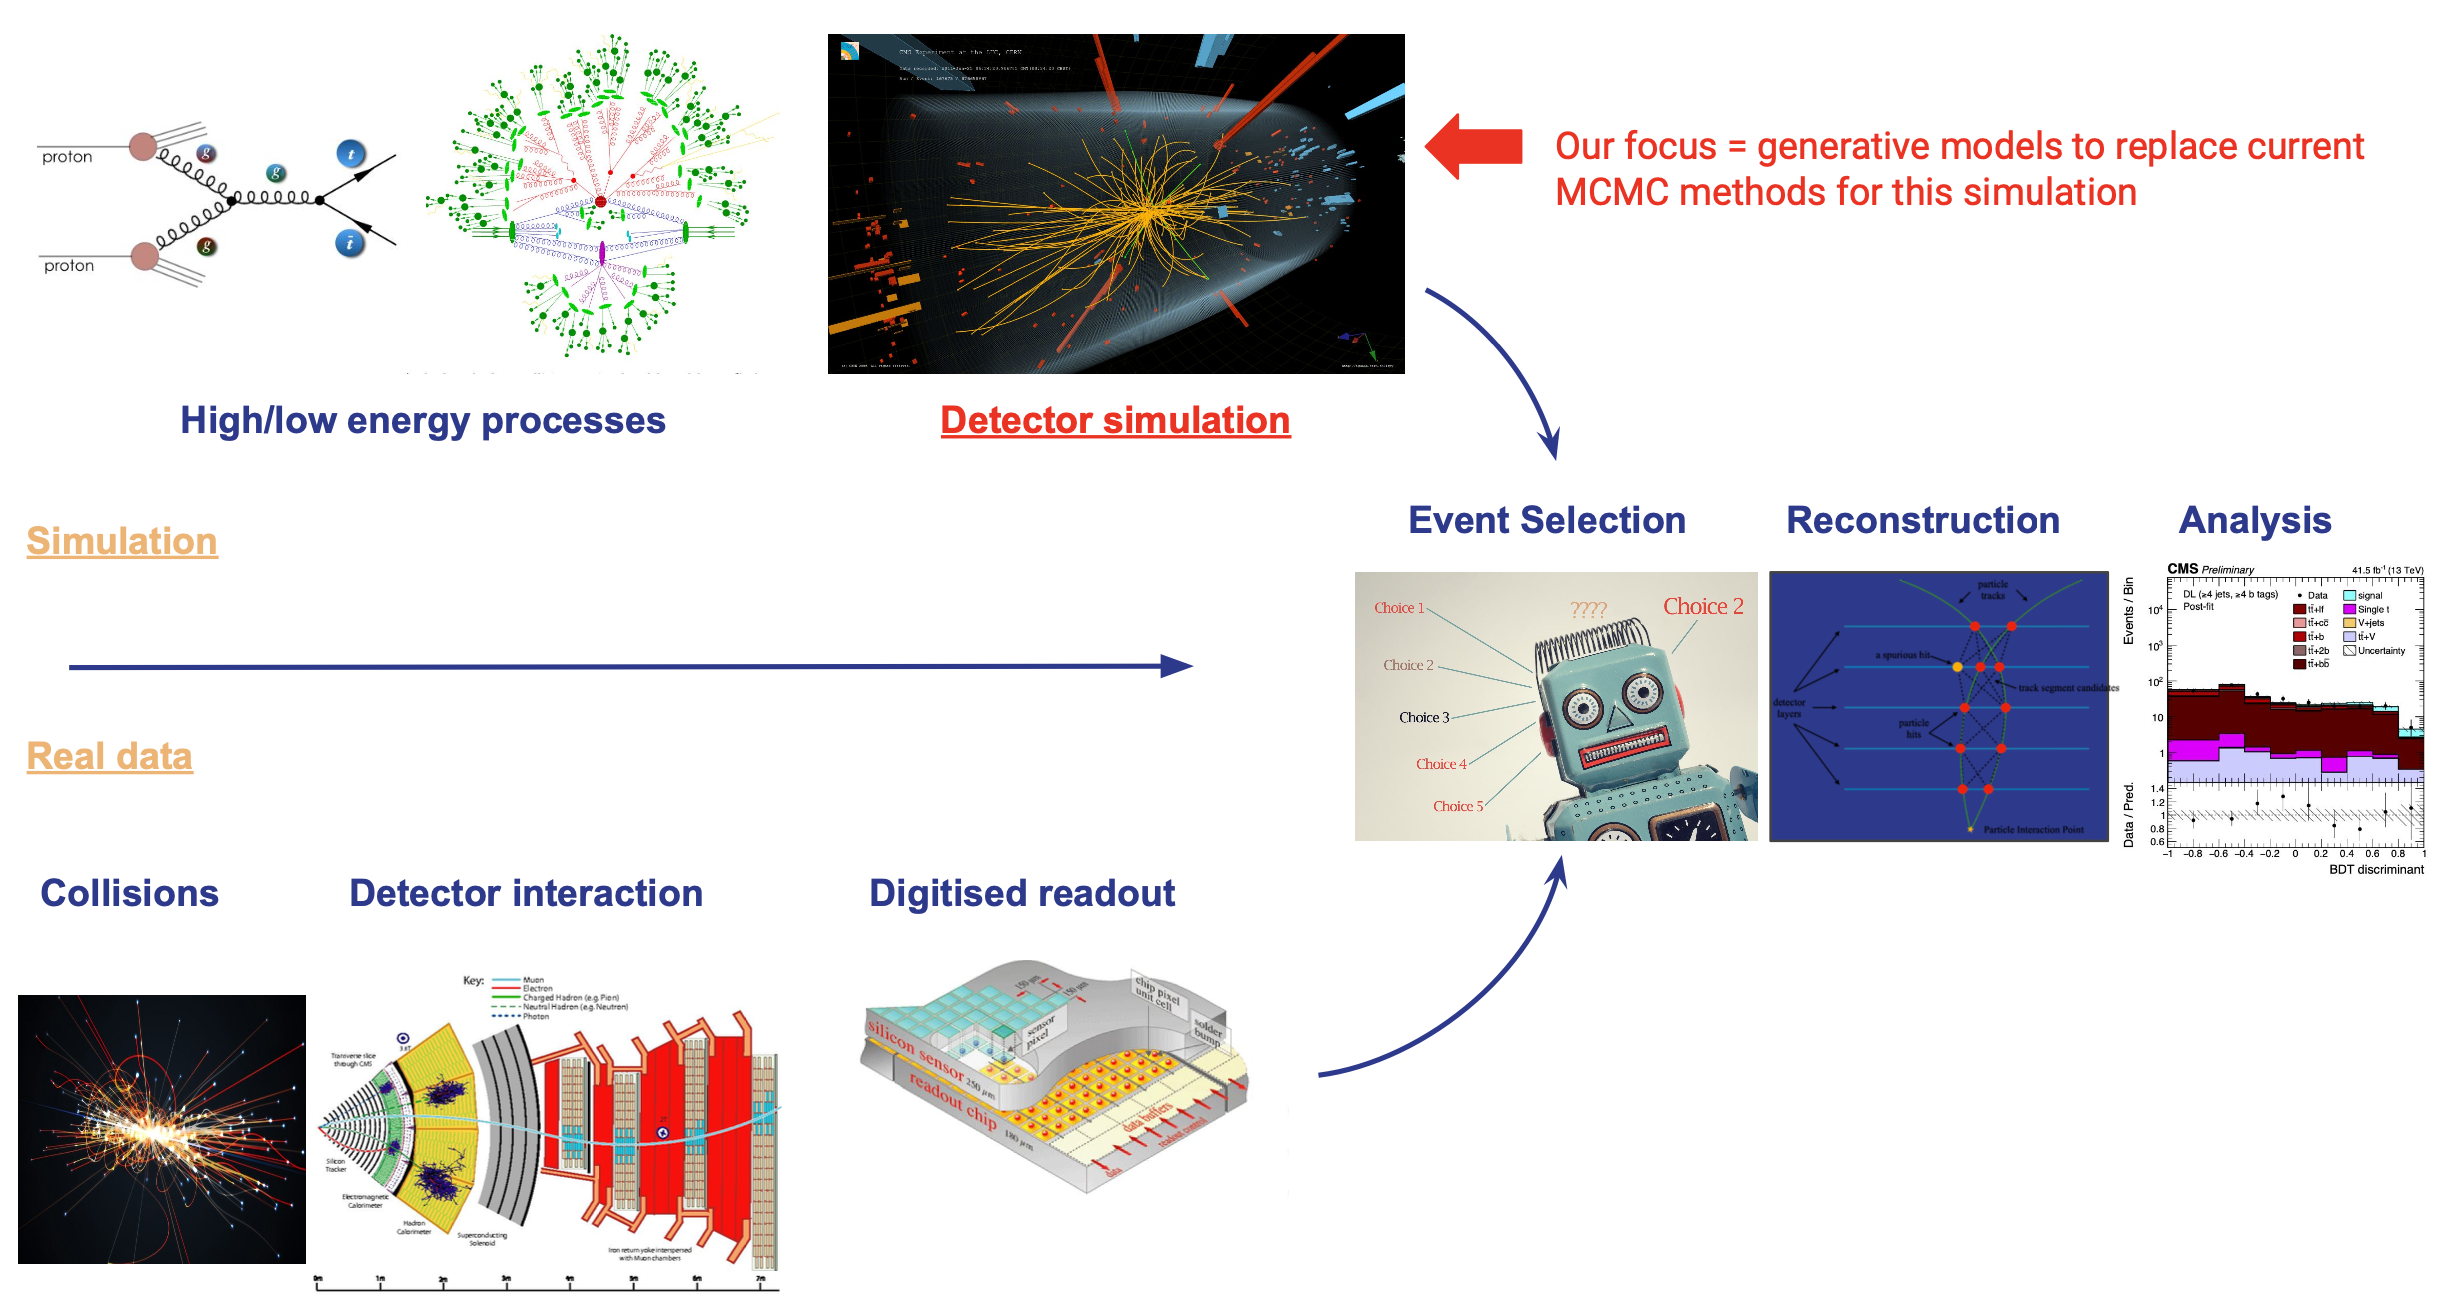
\includegraphics[width=0.7\textwidth]{Figures/simulation.png}
    \caption{The importance of simulation. Credit: Joshuha Thomas-Wilsker}
    \label{fig:fig1}
    \end{figure}

\subsection{Generative Models for Fast Simulation}
To address these challenges, generative models—particularly diffusion models—have emerged as promising alternatives for accelerating simulation while maintaining accuracy. Instead of replacing Geant4 entirely, the goal is to find an optimal balance between speed and precision, as illustrated in Figure \ref{fast}. Recent works, such as Yang et al.'s score-based models~\cite{song2020} and diffusion-based calorimeter simulations~\cite{mikuni2021}, have significantly reduced computation time while preserving fidelity. Building on these advances, our project introduces a novel model that generates 3D point clouds representing energy distributions across spatial coordinates in a single step. Unlike previous models, which often focus on one-dimensional projections (e.g., energy vs. z-coordinate), our approach captures full 3D distributions in a single forward pass, enabling rapid and comprehensive simulations suited to high-luminosity experiments.

Deep learning offers a compelling alternative to traditional parametric models, with generative techniques such as Generative Adversarial Networks (GANs)~\cite{goodfellow2014}, Variational Autoencoders (VAEs)~\cite{kingma2013}, and Normalizing Flows (NFs) ~\cite{dinh2016} increasingly adopted for fast detector simulations. GANs, for example, have demonstrated considerable success in generating calorimeter showers~\cite{paganini2018} and are now integrated into the ATLAS fast simulation framework~\cite{atlas2018}. However, they present optimization challenges and can suffer from mode collapse, where the generator fails to fully capture data diversity. NFs, while offering stable training and accurate density estimation, remain computationally expensive for high-dimensional data, limiting their feasibility for complex detector simulations. Additionally, their rigid model structure further constrains adaptability~\cite{verheyen2021, verheyen2021b}.

\subsection{Score-Based Generative Models for Simulation}
This work explores score-based generative models~\cite{song2020}, which learn the gradient of the data density rather than the density itself. This approach allows for more flexible network architectures without requiring Jacobian computation during training, enabling the use of bottleneck layers to reduce trainable parameters and improve scalability. Recent advancements in score-based models have demonstrated their potential in calorimeter simulation, achieving a balance between high-dimensional fidelity and computational efficiency—making them suitable for ultra-fine calorimeters and complex datasets~\cite{cms2017, cms2018}.

By leveraging score-based models, our project aims to address both the computational challenges of high-luminosity LHC experiments and the limitations of traditional fast simulation methods. Our approach enhances accuracy by capturing full 3D spatial distributions while significantly reducing simulation time, offering a scalable and reliable solution for next-generation collider experiments.

\begin{figure}[H]
\centering
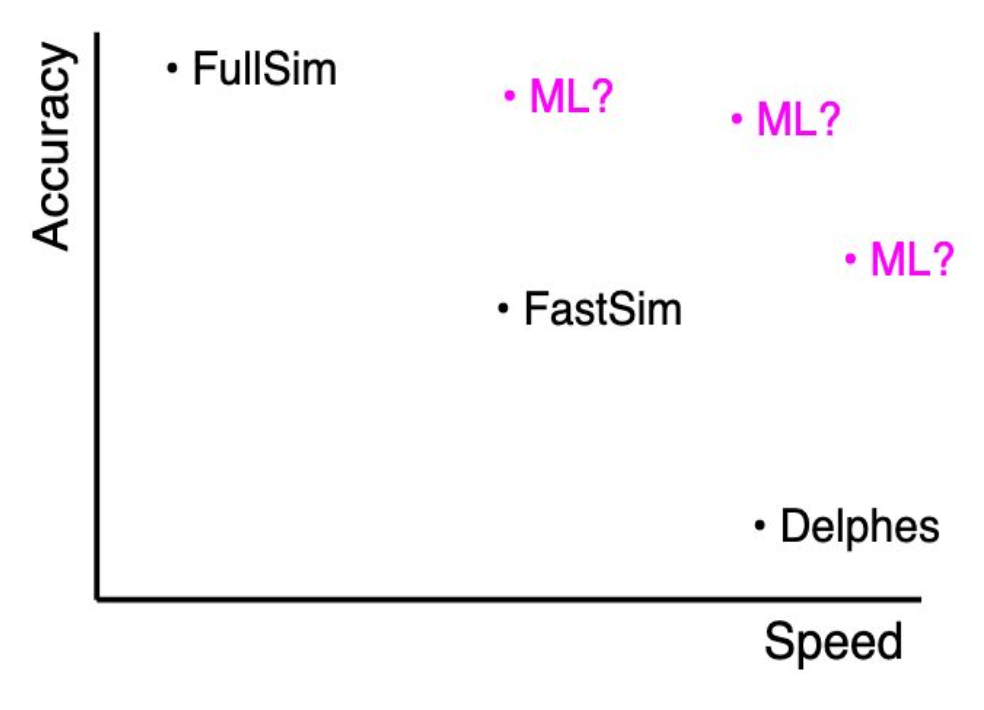
\includegraphics[width=0.7\textwidth]{Figures/fast.png}
\caption{The balance between accuracy and speed in simulation. Credit: Joshuha Thomas-Wilsker}
\label{fast}
\end{figure}

\section{Challenges}

Generating a 3D point cloud to accurately model energy deposition across spatial coordinates presents several key challenges. Traditional approaches primarily focus on one-dimensional projections, modeling energy as a function of a single spatial dimension. While effective for simplified representations, these methods fail to capture the full complexity of particle interactions. Our model, in contrast, aims to reconstruct the complete three-dimensional energy distribution in a single forward pass, requiring a delicate balance between high-dimensional fidelity and computational efficiency.

To achieve this, we integrate advanced architectural components, including Gaussian Fourier Projection for time encoding and mean-field attention mechanisms with a class token, along with conditional guidance based on incident energy. These features enable precise control over both positional and energy distributions, addressing the intricate dependencies within the 3D spatial domain. However, training a model to learn the complex correlations between spatial coordinates, energy deposition, and incident energy introduces significant computational challenges. Ensuring that the model generalizes well across various particle types and energies, while maintaining efficiency, remains a non-trivial task.

The high-dimensional nature of this generative task demands careful conditioning to reflect realistic energy variations across spatial coordinates. Our approach requires the model to dynamically adjust its predictions based on incident energy, detector response, and local correlations. This complexity leads to a tradeoff: increasing fidelity often incurs substantial computational
costs. Optimizing the architecture to maintain accuracy while reducing inference time is a key focus of our work.

Despite these challenges, our optimized approach achieves up to a 500-fold speedup over traditional Geant4-based simulations, offering a scalable alternative suited for next-generation collider experiments. By leveraging modern generative techniques, we not only enhance simulation efficiency but also improve the resolution and realism of synthetic data.

In summary, our model represents a step forward in 3D point cloud generation for high-energy physics simulations. By bridging the gap between scalability and fidelity, we address the computational limitations of conventional methods while enabling high-precision modeling of energy deposition patterns. These advancements pave the way for more efficient and realistic simulations, crucial for meeting the demands of high-luminosity experiments and future discoveries in particle physics.


% % Chapter 2. Detector
\chapter{Detector}

\section{The Large Hadron Collider (LHC)}
Although the Standard Model of particle physics has been remarkably successful up to TeV scale, several fundamental questions remain unanswered. The Large Hadron Collider (LHC) at CERN is the most powerful particle accelerator ever built, designed to explore above the TeV energy scale. It consists of a 27-kilometer ring of superconducting magnets and accelerating structures, enabling proton-proton collisions at an unprecedented energy of 13 TeV (design energy of 14 TeV). The main purpose of the LHC is to explore the electroweak symmetry breaking for which the Higgs mechanism is presumed to be responsible and search for new physics beyond the Standard Model.
\begin{figure}[ht]
    \centering
    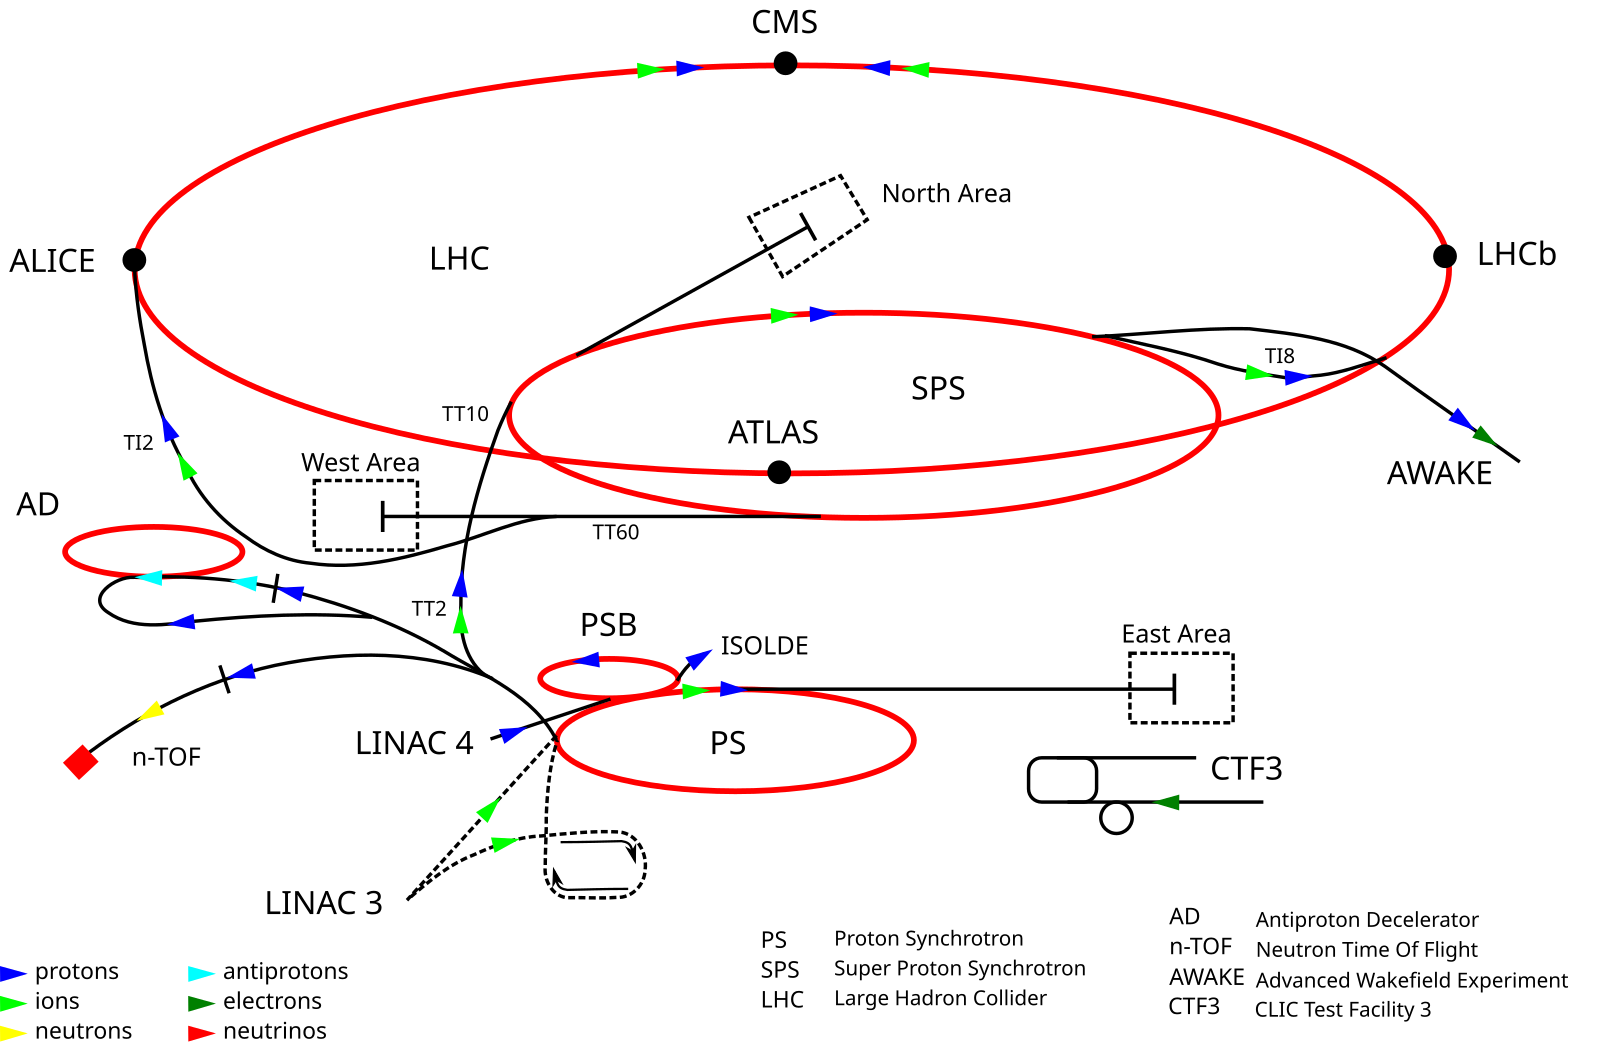
\includegraphics[width=0.8\textwidth]{Figures/Cern_Accelerator_Complex.png} % Replace with your LHC diagram file
    \caption{The schema of LHC} ~\cite{lhc_picture}
    \label{fig:lhc}
\end{figure}

The LHC features a high collision rate with 25 ns bunch spacing, producing up to $10^9$ interactions per second. The facility includes key experimental sites like CMS, ATLAS, LHCb, and ALICE, each optimized for specific research goals. The injection system consists of the Proton Synchrotron (PS) and Super Proton Synchrotron (SPS), ensuring high beam luminosity and energy.

\subsection{Key Components of the LHC}

\subsubsection{Injector Chain}
The LHC relies on a sequence of pre-accelerators to prepare the particle beams:
\begin{itemize}
    \item \textbf{Linear Accelerator (Linac4):} Replaced Linac2 and accelerates negative hydrogen ions (H$^-$) to 160 MeV. Synchrotron Booster (PSB). \cite{linac4}
    \item \textbf{Proton Synchrotron Booster (PSB):} Strips electrons from H$^-$ ions to produce protons and accelerates them to 2 GeV. \cite{psb}
    \item \textbf{Proton Synchrotron (PS):} Further increases the beam energy to 26 GeV.\cite{ps}
    \item \textbf{Super Proton Synchrotron (SPS):} Boosts the energy of protons to 450 GeV before injection into the LHC.\cite{sps}
\end{itemize}
Each stage ensures the beam achieves the required energy, intensity, and quality, culminating in proton-proton collisions at 13.6 TeV in the LHC in Run3.

\subsubsection{Main Ring}
The LHC ring consists of two counter-rotating beam pipes, maintained under ultrahigh vacuum conditions to avoid particle collisions with residual gas.
\begin{itemize}
    \item \textbf{Superconducting Magnets:} Approximately 1,232 dipole magnets steer the beams around the circular path, while quadrupole magnets focus them to maintain stability. \cite{superconducting}
    \item \textbf{Cryogenics:} The superconducting magnets operate at 1.9 Kelvin (-271\degree C), achieved using liquid helium cooling systems. \cite{lhc_2024}
\end{itemize}

\subsubsection{Experimental Sites}
The LHC includes four main experiments, strategically placed along the ring:
\begin{itemize}
    \item \textbf{CMS (Compact Muon Solenoid):} Focused on studying high-energy collisions for precision measurements and new physics.
    \item \textbf{ATLAS (A Toroidal LHC Apparatus):} Another general-purpose detector designed for broad physics exploration.
    \item \textbf{ALICE (A Large Ion Collider Experiment):} Specializes in studying heavy-ion collisions and the quark-gluon plasma.
    \item \textbf{LHCb (LHC Beauty Experiment):} Dedicated to investigating the matter-antimatter asymmetry by studying b-hadron decays.
\end{itemize}

\subsubsection{Collimation and Beam Dumps}
The LHC is equipped with a sophisticated collimation system to remove stray particles and protect sensitive components. Beam dumps allow controlled termination of particle beams after experiments or emergencies.

\subsubsection{Collision Points}
Particles are brought to collision points within the detectors, achieving a luminosity of $10^{34}~\mathrm{cm^{-2}s^{-1}}$. These conditions facilitate rare particle processes, such as Higgs boson production.

\subsection{Technological Challenges}
\begin{itemize}
    \item \textbf{Radiation Damage:} Extensive shielding is required to protect equipment and personnel from high levels of radiation.
    \item \textbf{Alignment Precision:} The alignment of the LHC's components must be maintained within micrometers to ensure proper beam steering.
    \item \textbf{Data Volume:} Experiments generate petabytes of data annually, necessitating advanced computational infrastructure for storage and analysis.
\end{itemize}

The LHC represents a pinnacle of human engineering and scientific collaboration, involving thousands of scientists and engineers worldwide.

\section{The Compact Muon Solenoid (CMS)}
CMS is a general-purpose detector optimized for high-precision measurements and searches for rare physics events. The detector design focuses on:
\begin{itemize}
    \item Precise tracking for charged particles.
    \item High-resolution electromagnetic and hadronic calorimetry.
    \item Efficient muon identification and momentum resolution.
    \item Robust missing transverse energy measurement.
\end{itemize}

\begin{figure}[ht]
    \centering
    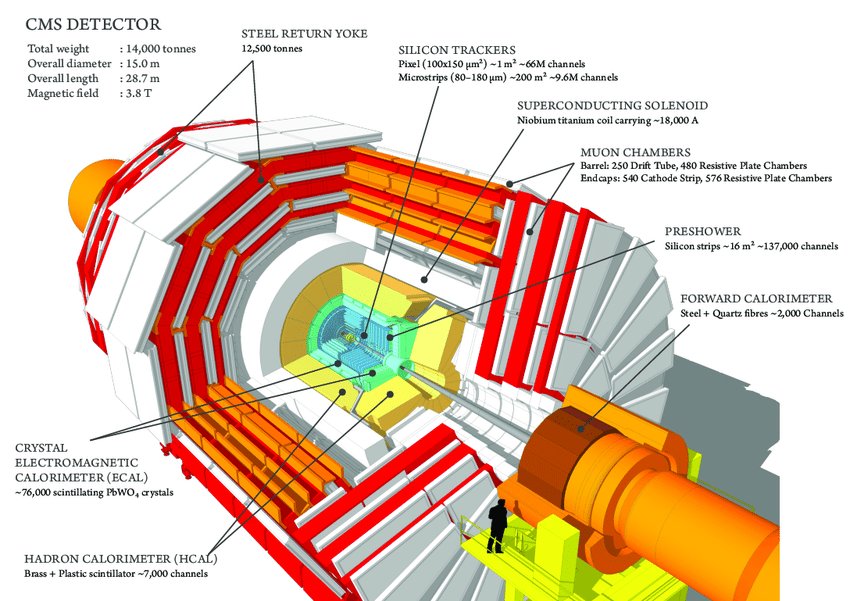
\includegraphics[width=0.8\textwidth]{Figures/CMS Detector Schematic.png} % Replace with a CMS diagram
    \caption{Exploded view of the CMS detector, showing its main components.}
    \label{fig:cms_detector}
\end{figure}

In order to detect the momentum of muons  The CMS detector features a 4 Tesla superconducting solenoid with a 6-meter diameter and 12.5-meter length, providing a strong magnetic field essential for accurate momentum measurements of charged particles. The solenoid is enclosed inside a 10,000-tonne iron return yoke, which serves to contain the magnetic field and also houses the muon detection system.\cite{superconducting_magnet} The CMS muon spectrometer is based on gaseous detectors placed inside the iron return yoke of the superconducting solenoid.\cite{4436524}

In order to better illustrate the CMS detector, the figure below is the Cross-sectional schematic of the CMS detector showcasing its key components: the Silicon Tracker, Electromagnetic Calorimeter (ECAL), Hadron Calorimeter (HCAL), and Superconducting Solenoid.

\begin{figure}[ht]
    \centering
    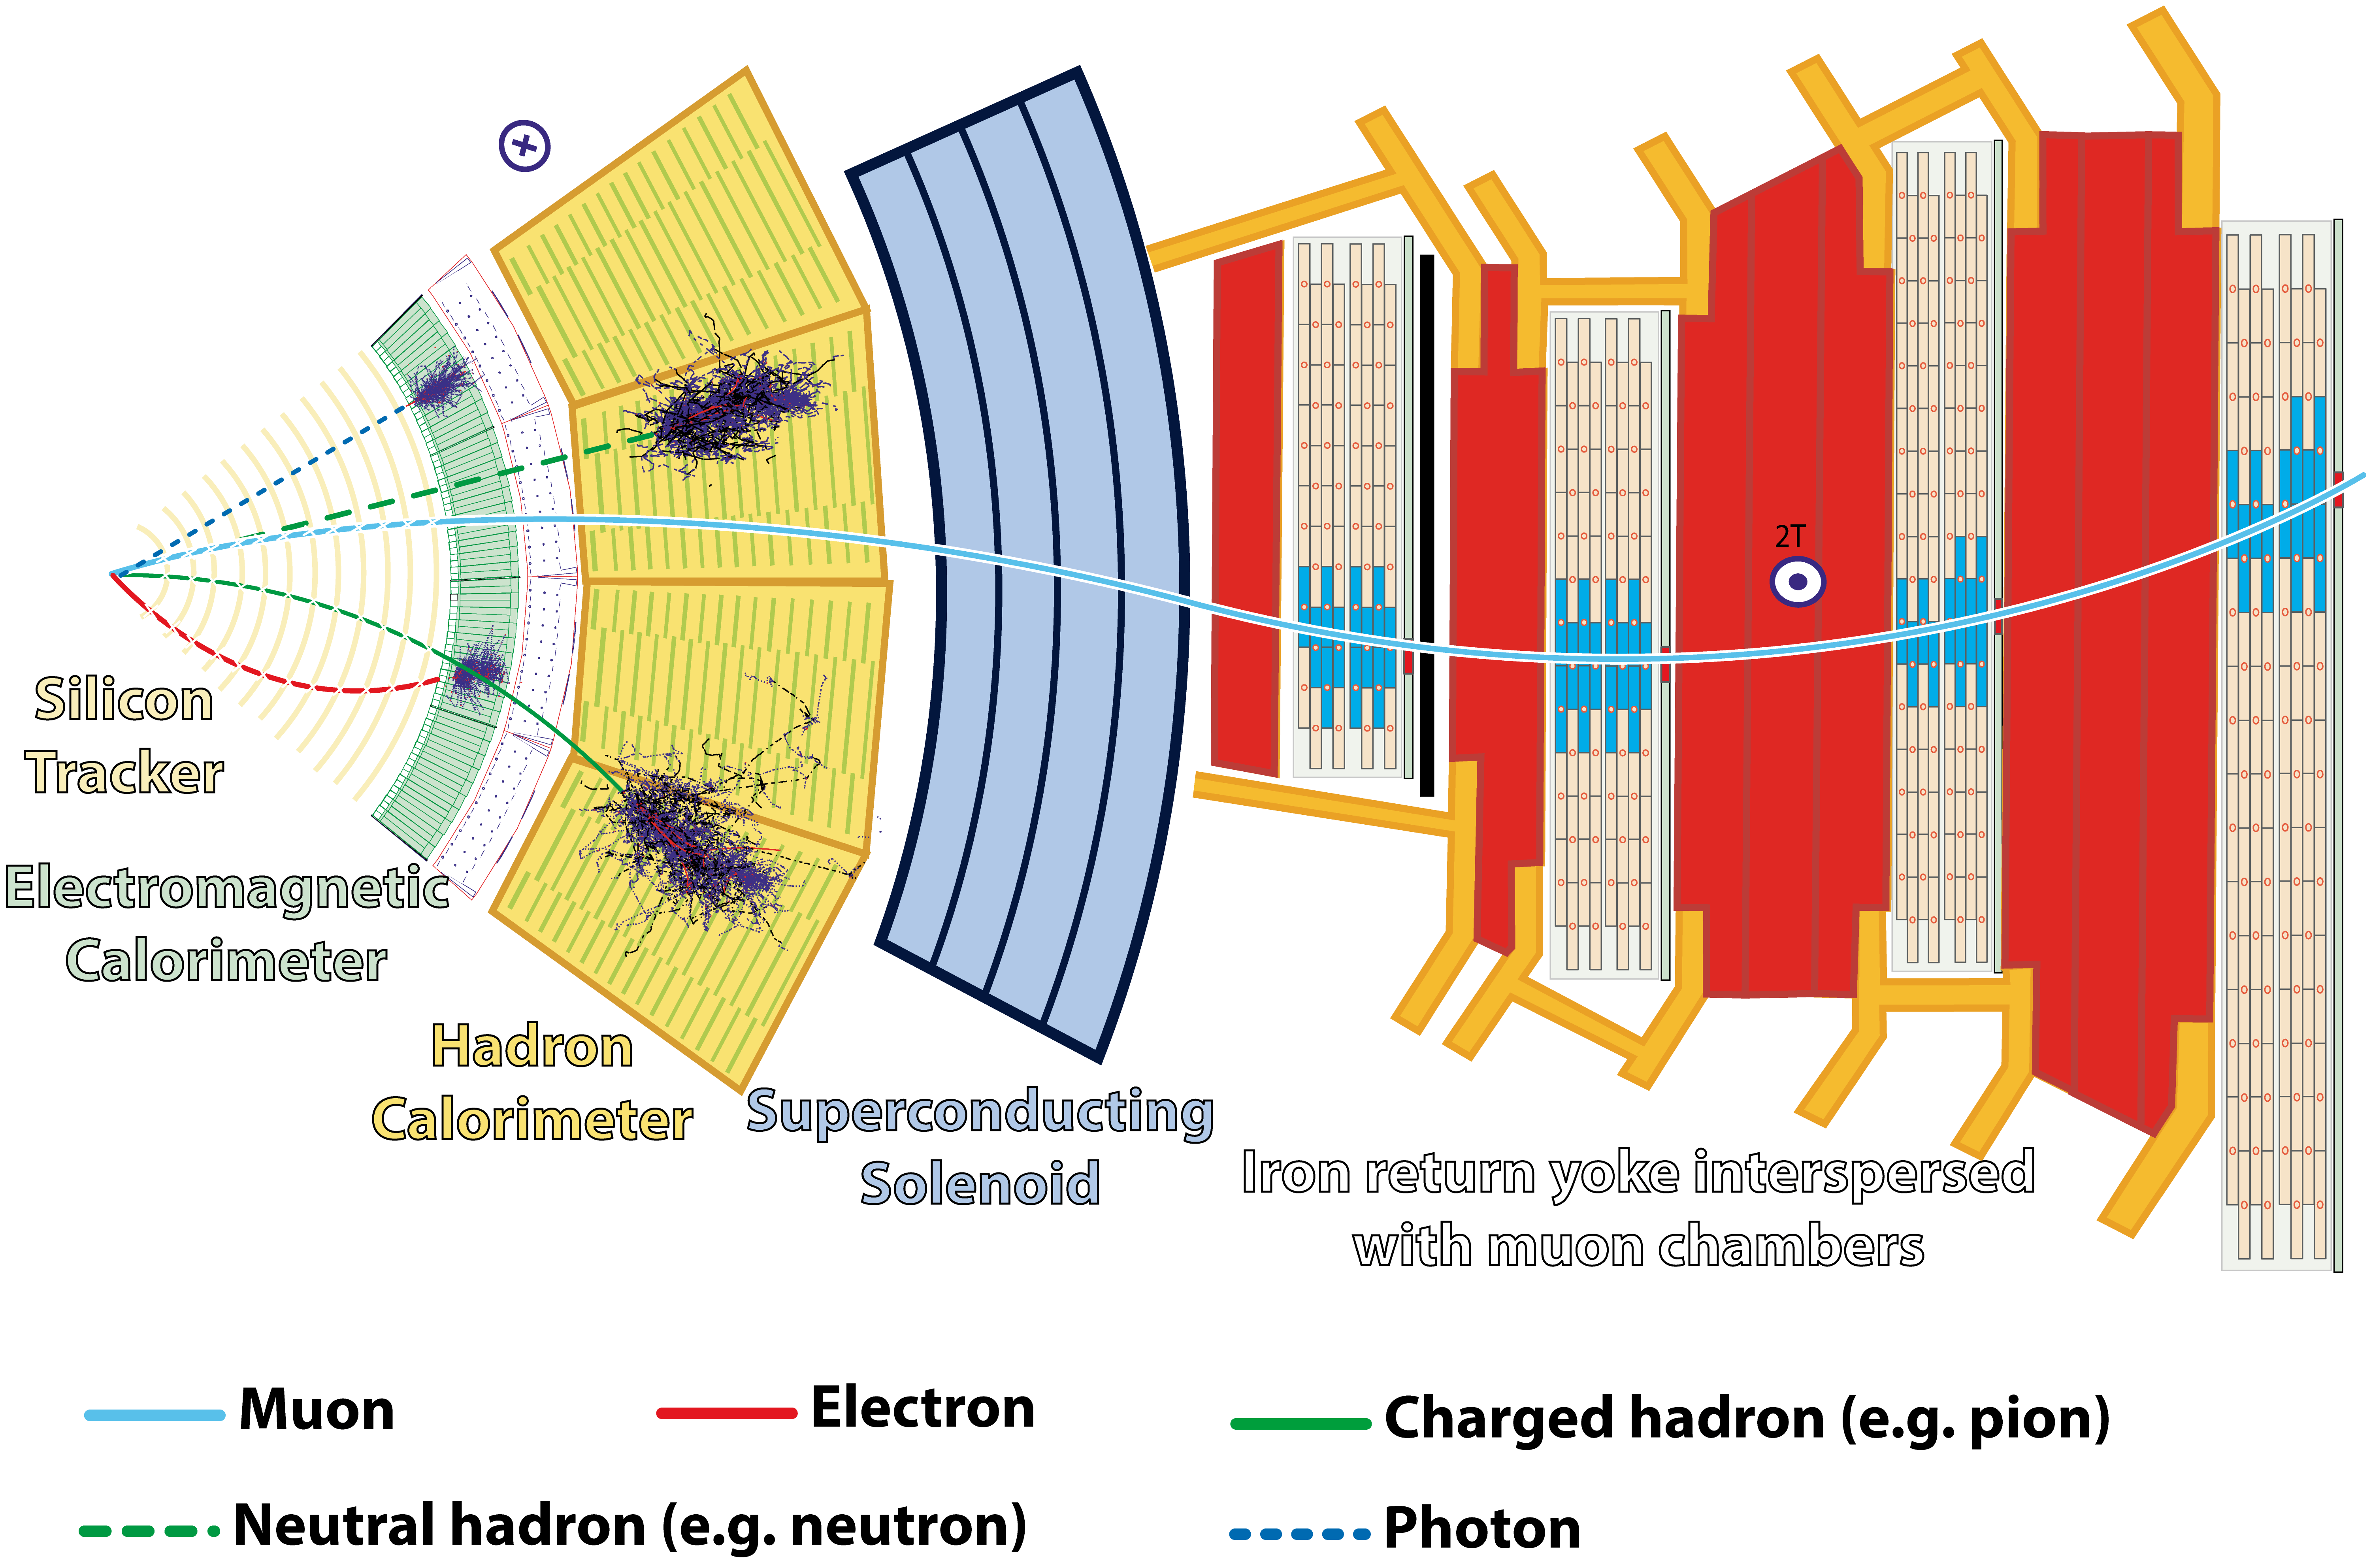
\includegraphics[width=0.8\textwidth]{Figures/CMS Slice White Background.png} % Replace with a Tracker diagram
    \caption{Cross-sectional schematic of the CMS detector}
    \label{fig:cms_tracker}
\end{figure}

\section{Silicon Tracker}

The tracker system in the CMS detector is designed to reconstruct the trajectories of charged particles produced in high-energy collisions with unparalleled precision. This subsystem plays a vital role in measuring the momentum of particles, identifying particle types, and reconstructing primary and secondary vertices.

\subsection{Silicon Pixel Detector}
The innermost layer of the tracker is the silicon pixel detector, which provides high-resolution tracking near the interaction point. It consists of three barrel layers and two endcap disks on either side, covering a pseudorapidity range of $|\eta| < 2.5$ \cite{tracker_tdr}. The pixel detector is constructed using silicon sensors segmented into millions of tiny pixels, each measuring $100\times150~\mu m^2$.

The pixel detector is designed to withstand intense radiation levels and high particle flux near the beamline. Its fine granularity ensures excellent spatial resolution, which is critical for identifying displaced vertices from the decays of short-lived particles such as $B$-mesons and $	au$ leptons ~\cite{pixels}.

\subsection{Silicon Strip Tracker}
Surrounding the pixel detector is the silicon strip tracker, which extends the tracking coverage to larger radii and provides additional layers for trajectory reconstruction. The strip tracker is divided into the Tracker Inner Barrel (TIB), Tracker Outer Barrel (TOB), Tracker Endcaps (TEC), and Tracker Inner Disks (TID). These components collectively cover a radial distance of 20 to 110 cm from the beamline \cite{tracker_tdr}.

The silicon strips are oriented in parallel arrays, with each strip measuring several centimeters in length and a few hundred microns in width. By combining signals from multiple layers, the strip tracker achieves precise momentum measurements and improves the robustness of the trajectory reconstruction. \cite{strips}

\subsection{Material Choices and Performance}
The tracker is constructed entirely from silicon sensors, chosen for their excellent resolution and radiation hardness. Key considerations in the design include:
\begin{itemize}
    \item \textbf{Lightweight support structures:} Minimize material interactions that can scatter particles and degrade tracking performance.
    \item \textbf{Radiation-tolerant electronics:} Ensure reliable operation in the high-radiation environment of the LHC.
    \item \textbf{High granularity:} Allows for precise reconstruction of particle trajectories even in the presence of multiple simultaneous collisions (pile-up).
\end{itemize}

The tracker achieves a transverse momentum resolution of approximately $\Delta p_T / p_T = 1\%$ for particles with $p_T$ around $100~\mathrm{GeV/c}$. This precision enables detailed studies of particle properties, including invariant mass reconstruction and decay vertex identification \cite{tracker_tdr}.

% \begin{figure}[ht]
%     \centering
%     %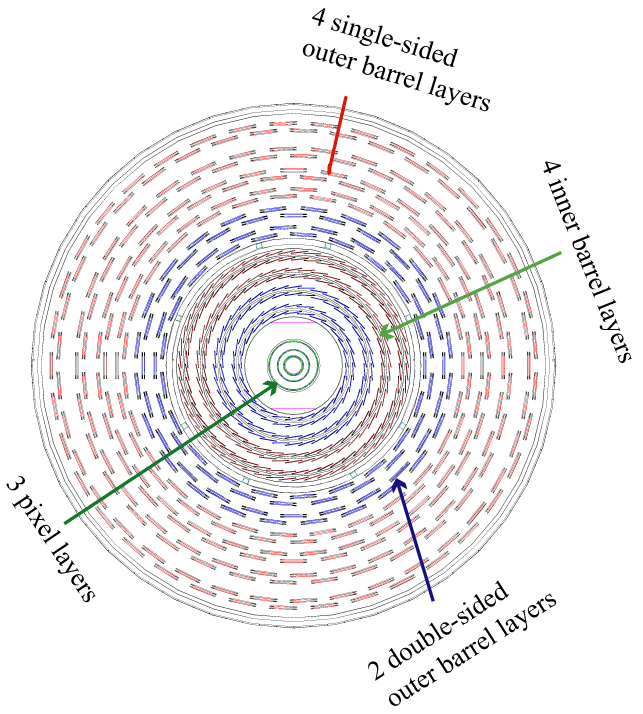
\includegraphics[width=0.8\textwidth]{Figures/Barrel.png} % Replace with a Tracker diagram
%     \caption{Cross-sectional schematic of the CMS tracker, showing the pixel and strip components.}
%     \label{fig:cms_tracker}
% \end{figure}

% \begin{figure}[ht]
%     \centering
%     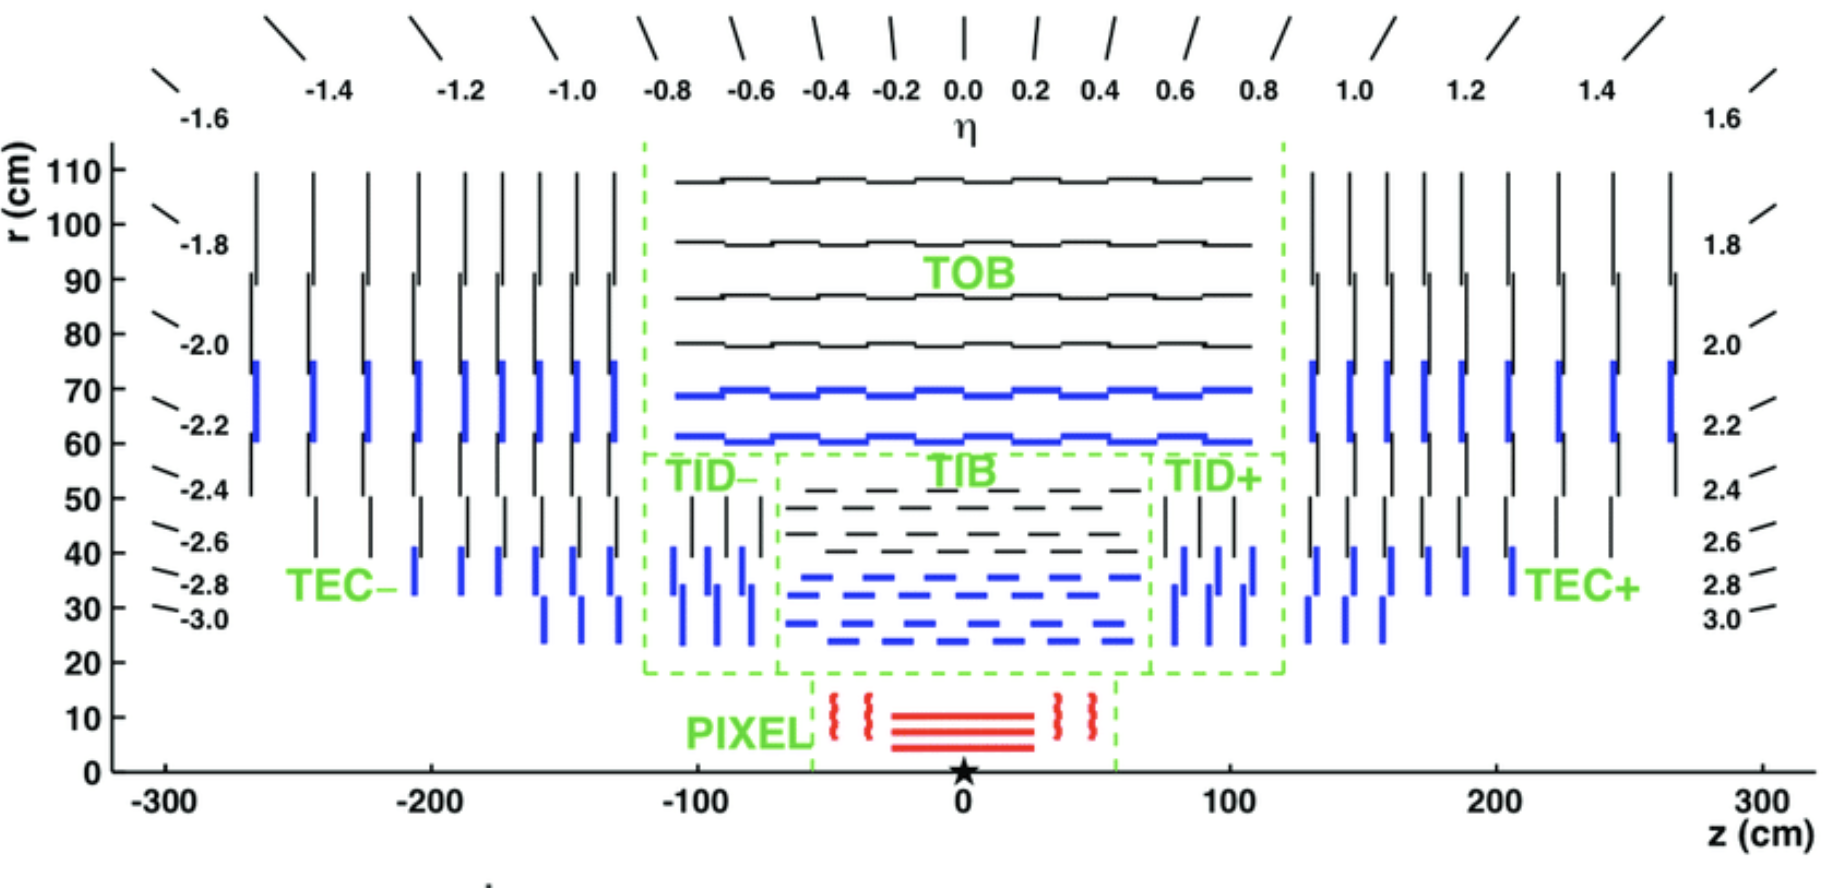
\includegraphics[width=0.8\textwidth]{Figures/tracker_cross.png} % Replace with a Tracker diagram
%     \caption{Cross-sectional schematic of the CMS tracker, showing the pixel and strip components.}
%     \label{fig:cms_tracker}
% \end{figure}

The tracker is designed to withstand high radiation levels and provides a momentum resolution of $\Delta p_T / p_T \approx 1\%$ for particles with $p_T \sim 100~\mathrm{GeV/c}$. The low-mass design minimizes material interactions, reducing the impact on photon and electron measurements. Cooling systems maintain stable operation despite the intense radiation environment.

\section{Electromagnetic Calorimeter (ECAL)}
% The ECAL measures the energy of photons and electrons with high precision. It consists of lead tungstate (PbWO$_4$) crystals, optimized for:
% \begin{itemize}
%     \item Fast response time ($<25~\mathrm{ns}$).
%     \item Radiation hardness.
%     \item Fine granularity for excellent position resolution.
% \end{itemize}



% \subsection{Barrel and Endcap Structure}
% The ECAL is divided into the barrel (EB) and two endcaps (EE), covering $|\eta| < 3.0$. The barrel consists of 36 supermodules, each containing thousands of crystals aligned quasi-projectively to the interaction point. The endcaps extend the coverage to higher pseudorapidities, crucial for forward physics measurements.

% \subsection{Preshower Detector}
% Due to the structure of parallel alignment of crystals in the endcaps, the ECAL has a lower granularity in the endcaps than in the barrel. In order to improve the sensitivity of track of the photons. The endcaps include a preshower detector, comprising two layers of silicon strip sensors placed behind lead converters. This subsystem enhances the discrimination between photons and neutral pions by measuring the photon conversion probability.


% \subsection{Performance}
% Energy resolution is parameterized as:\cite{cms_tdr_ecal}
% \[
% \frac{\sigma_E}{E} = \frac{S}{\sqrt{E}} \oplus \frac{N}{E} \oplus C,
% \]
% where $S$, $N$, and $C$ are the stochastic, noise, and constant terms, respectively. The ECAL achieves an exceptional energy resolution of approximately 1\% for electrons and photons at $E = 100~\mathrm{GeV}$.

The Electromagnetic Calorimeter (ECAL) in the CMS detector is a crucial subsystem designed to measure the energy of electrons and photons with high precision. The ECAL achieves this by utilizing scintillating lead tungstate (PbWO$_4$) crystals as the active medium, coupled with photodetectors to convert scintillation light into electrical signals. Its design, divided into the Barrel (EB), Endcap (EE), and Preshower Detector (ES), ensures optimal performance across a wide range of pseudorapidity. In this research, because our dataset is mainly focused on photons and electrons, the ECAL is actually the region we mainly focus on. In later Chapter, the detector we called is actually reference to the ECAL.

\subsection{The ECAL Barrel (EB)}
The ECAL Barrel covers the central pseudorapidity region, $|\eta| < 1.479$, and consists of approximately 61,200 PbWO$_4$ crystals. These crystals are characterized by their high density, fast scintillation time, and radiation hardness \cite{ecal_tdr}. Lead tungstate is chosen due to its high density and short radiation length, which allows electromagnetic showers to develop within a compact volume. This compactness ensures that the ECAL can achieve high resolution while fitting within the spatial constraints of the CMS detector.

Each crystal is aligned quasi-projectively towards the interaction point, ensuring minimal gaps in coverage and precise angular resolution. The scintillation light produced in the crystals is detected by avalanche photodiodes (APDs) for the barrel region, which offer excellent sensitivity and radiation resistance \cite{ecal_tdr}.

\subsection{The ECAL Endcap (EE)}
The ECAL Endcap extends the coverage of the ECAL to higher pseudorapidities, from $|\eta| = 1.479$ to $|\eta| = 3.0$. The endcap region is composed of roughly 14,600 PbWO$_4$ crystals, arranged in a geometry optimized for forward physics studies \cite{ecal_tdr}. Due to the higher radiation levels and particle flux in this region, the photodetectors used are vacuum phototriodes (VPTs), which are more robust against radiation damage compared to APDs.

The higher radiation environment in the endcap region also necessitates additional cooling and monitoring systems to maintain the performance of the crystals and photodetectors. The EE plays a critical role in measuring photons and electrons produced at small angles relative to the beamline, ensuring comprehensive detector coverage \cite{ecal_tdr}.

\subsection{The Preshower Detector}
The preshower detector is located in front of the ECAL Endcaps and is designed to enhance the discrimination between photons and neutral pions ($\pi^0$). It consists of two layers of lead absorbers, interleaved with silicon strip sensors \cite{ecal_tdr_preshower}. The lead layers initiate electromagnetic showers, while the silicon sensors measure the spatial distribution of the resulting particles.

This design allows the preshower detector to effectively distinguish between single photons and $\pi^0$ decays, which produce two closely spaced photons. This capability is crucial for improving the ECAL's performance in identifying isolated photons in a high-particle-density environment \cite{ecal_tdr_preshower}.

\begin{figure}[ht]
    \centering
    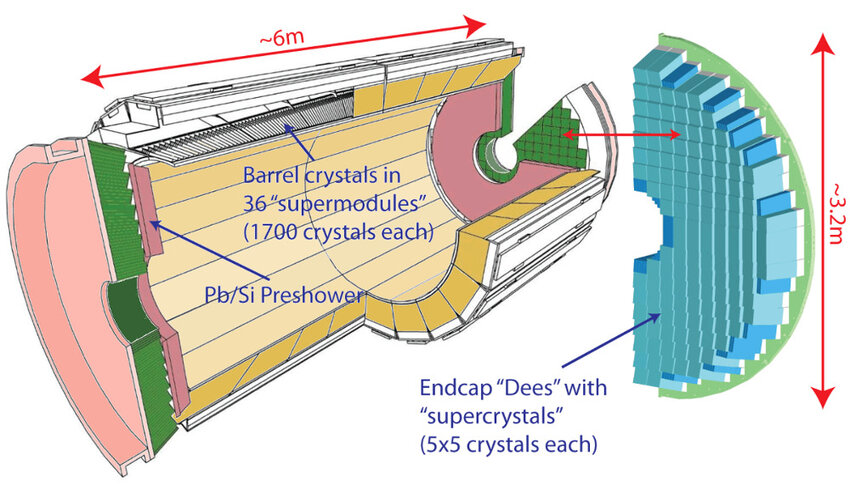
\includegraphics[width=0.8\textwidth]{Figures/ECAL Schematic Overview.png} % Replace with an ECAL diagram
    \caption{Structure of the ECAL showing barrel and endcap regions.} ~\cite{ECAL}
    \label{fig:ecal}
\end{figure}

\subsection{Material Choices and Performance}
The choice of PbWO$_4$ as the active material for the ECAL is driven by its unique properties:
\begin{itemize}
    \item \textbf{High density and short radiation length:} These properties allow electromagnetic showers to be contained within a compact volume, ensuring precise energy measurements.
    \item \textbf{Fast scintillation time:} PbWO$_4$ crystals have a decay time of approximately 25 ns, matching the LHC's bunch crossing interval \cite{ecal_tdr}.
    \item \textbf{Radiation hardness:} PbWO$_4$ is resistant to radiation damage, which is critical for maintaining detector performance over extended periods of operation.
\end{itemize}

The ECAL achieves an excellent energy resolution, parameterized as:

\[
\frac{\sigma_E}{E} = \frac{S}{\sqrt{E}} \oplus \frac{N}{E} \oplus C,
\]

where $S$ is the stochastic term, $N$ represents the noise, and $C$ is the constant term \cite{ecal_tdr}. This resolution allows the ECAL to distinguish between different particle species and measure their energies with high precision, making it an indispensable tool for studies of Higgs boson decays, rare processes, and new physics searches.

\section{Hadronic Calorimeter (HCAL)}
The HCAL measures hadronic energy, complementing the ECAL in reconstructing jets and missing transverse energy. It employs a sampling design with brass absorbers and plastic scintillators.

The Hadronic Calorimeter (HCAL) in the CMS detector is an essential component designed to measure the energy of hadrons produced in high-energy collisions. The HCAL achieves this through a carefully engineered combination of absorber and active materials, divided into distinct regions optimized for different pseudorapidity ranges. These regions include the HCAL Barrel (HB), HCAL Endcap (HE), HCAL Forward (HF), and HCAL Outer (HO). The selection of materials and their specific configurations in each section is driven by the requirements of energy containment, radiation hardness, and detector efficiency.

\subsection{The HCAL Barrel (HB)}
The HCAL Barrel is the central component of the HCAL, covering the region close to the interaction point with a pseudorapidity range of $|\eta| < 1.3$. The HB is constructed using brass as the absorber material and plastic scintillators as the active medium. Brass is chosen due to its high density and structural stability, which allow it to efficiently stop high-energy hadrons and initiate hadronic showers.\cite{hcal_tdr} The dense nature of brass ensures that the hadronic showers are contained within a compact volume, which is critical for the limited space available in the detector.

The active medium in the HB consists of plastic scintillator tiles, which emit light when traversed by charged particles generated in the hadronic showers. This scintillation light is collected by photodetectors, such as silicon photomultipliers, and converted into an electrical signal proportional to the energy deposited in the calorimeter. The use of plastic scintillators ensures a fast response time, high light yield, and excellent linearity, all of which contribute to the precision of energy measurements.

\subsection{The HCAL Endcap (HE)}
The HCAL Endcap extends the coverage of the HCAL to higher pseudorapidities, from $|\eta| = 1.3$ to $|\eta| = 3.0$. Similar to the HB, the HE uses brass as the absorber material and plastic scintillators as the active medium. However, the endcap is designed to handle particles with higher momenta, which require increased thickness of the absorber layers to fully contain the hadronic showers.

The higher density and thickness of the brass absorbers in the HE ensure that the energy of the hadronic showers is completely absorbed, even for particles at extreme angles. The endcap region is critical for capturing the energy of forward jets and particles produced at small angles relative to the beamline, ensuring no significant gaps in the detector's acceptance.\cite{hcal_tdr}

\subsection{The HCAL Forward (HF)}
The HCAL Forward is specifically designed to handle the extreme forward region, covering $3.0 < |\eta| < 5.0$. This region experiences the highest particle flux and radiation levels, necessitating the use of radiation-hard materials such as steel for the absorbers and quartz fibers for the active medium. Steel is chosen for its durability and ability to withstand the intense radiation environment in the forward region. It also provides the density required to stop high-energy hadrons effectively.

The active medium in the HF consists of quartz fibers, which generate Cherenkov light when traversed by relativistic charged particles produced in the hadronic showers. Cherenkov light is collected by specialized photodetectors, providing a robust signal in an environment where plastic scintillators would suffer significant degradation. This combination of materials ensures that the HF maintains its performance over long periods of operation, even in the harshest conditions.

The HF plays a crucial role in studying forward physics phenomena, including parton distribution functions and diffractive events. Its design also contributes to the accurate measurement of missing transverse energy ($E_T^{\text{miss}}$) by reducing the likelihood of undetected particles escaping.\cite{hcal_tdr_forward}

\subsection{The HCAL Outer (HO)}
The HCAL Outer is located outside the superconducting solenoid and complements the energy measurements of the HB. The HO uses the steel return yoke of the solenoid as its absorber, with additional layers of plastic scintillators serving as the active medium. The primary purpose of the HO is to act as a "tail catcher," capturing energy from high-energy particles that pass through the HB and the solenoid without being fully absorbed.

Using the steel return yoke as an integral part of the calorimeter minimizes the overall size and weight of the detector while maintaining its energy containment capabilities. The additional scintillator layers ensure that any residual energy from penetrating particles is measured, providing a complete picture of the event's energy balance. \cite{hcal_tdr_outer}

\subsection{Material Choices and Their Impact}
The material choices for the HCAL are driven by the need to balance density, radiation hardness, and signal quality. Dense materials such as brass and steel are used to contain hadronic showers within a compact volume, minimizing leakage and ensuring precise energy measurements. Plastic scintillators are employed in regions with lower radiation exposure due to their high light yield and fast response time. In contrast, quartz fibers are used in the forward region, where their radiation tolerance and ability to generate Cherenkov light make them the ideal choice.

This careful selection of materials and their strategic placement within the HCAL ensures that the detector meets the stringent requirements for hadronic energy measurement. By providing accurate jet energy reconstruction and missing transverse energy measurements, the HCAL plays a vital role in the CMS detector's ability to explore physics at the energy frontier. \cite{hcal_cms_detector}

\begin{figure}[ht]
    \centering
    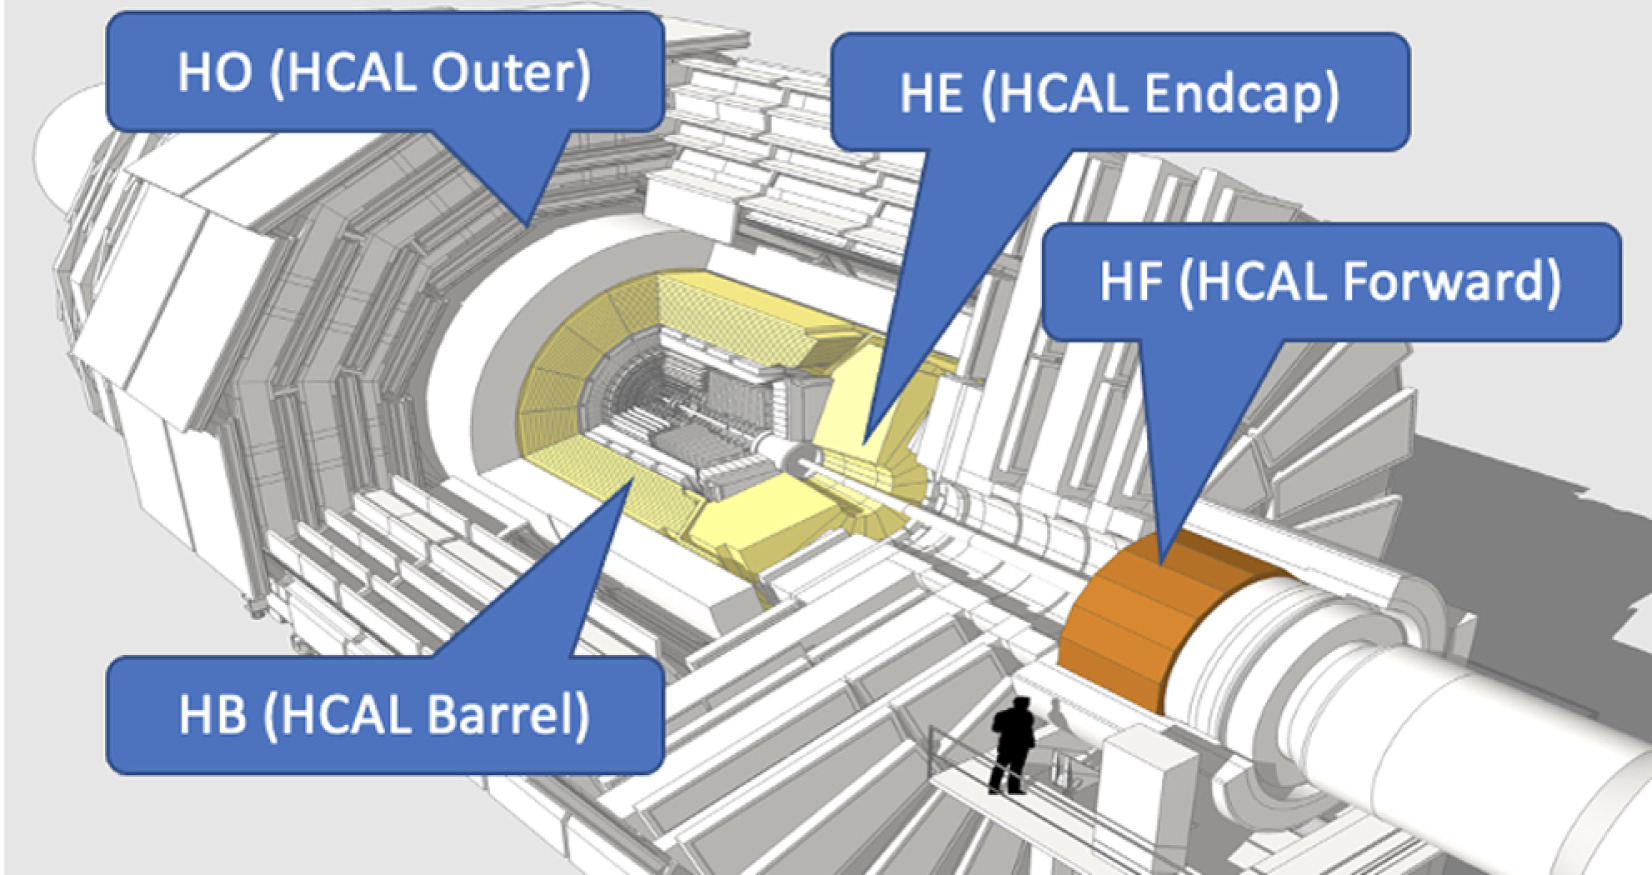
\includegraphics[width=0.8\textwidth]{Figures/HCAL.jpg} % Replace with an HCAL diagram
    \caption{Schematic of the HCAL with barrel, endcap, and forward sections.}
    \label{fig:hcal}
\end{figure}

\subsection{Performance}
The HCAL provides energy resolution of:\cite{cms_tdr_hcal}
\[
\frac{\sigma_E}{E} = \frac{S}{\sqrt{E}} \oplus C.
\]
The combination of ECAL and HCAL ensures accurate jet energy reconstruction and $E_T^{\text{miss}}$ measurements, critical for new physics searches.

\section{Muon Detector}
The muon detector in the CMS experiment is a crucial subsystem designed to identify and measure the momentum of muons, which are often key signatures in high-energy collisions. The muon system provides the outermost layer of the CMS detector, ensuring precise muon tracking and efficient triggering across a wide range of pseudorapidity.

\subsection{Muon Chambers: Drift Tubes (DT)}
Drift tubes are the primary technology used in the barrel region of the CMS detector, covering $|\eta| < 1.2$. They consist of gas-filled chambers with wires running along their length. When a muon passes through the chamber, it ionizes the gas, and the resulting electrons drift toward the central wire under the influence of an electric field \cite{muon_tdr}.

The time taken by the electrons to reach the wire allows for precise measurements of the muon's position. The DTs are arranged in layers, providing redundancy and improving spatial resolution. The use of drift tubes in the barrel region ensures robust performance in areas with lower radiation exposure and relatively uniform magnetic fields.

\subsection{Muon Chambers: Cathode Strip Chambers (CSC)}
Cathode strip chambers are employed in the endcap regions, where the pseudorapidity ranges from $1.2 < |\eta| < 2.4$. The CSCs are designed to operate in areas with higher radiation levels and non-uniform magnetic fields. They consist of multi-layered gas chambers with cathode strips and anode wires arranged perpendicularly \cite{muon_tdr}.

When a muon traverses a CSC, it ionizes the gas, and the resulting charge is collected on the strips and wires. The perpendicular arrangement allows for precise two-dimensional position measurements. This design ensures high efficiency and excellent spatial resolution in the endcap regions, where particle flux and radiation are more intense \cite{muon_tdr}.

\subsection{Resistive Plate Chambers (RPC)}
Resistive plate chambers are used in both the barrel and endcap regions, providing fast timing information and additional redundancy for triggering. RPCs consist of parallel resistive plates separated by a thin gas layer. When a muon passes through the gas, it creates an avalanche of electrons, resulting in a detectable signal \cite{muon_tdr}.

The fast response time of RPCs makes them ideal for the Level-1 trigger system, which is responsible for selecting events of interest in real time. Their simple design and robust performance contribute significantly to the overall efficiency of the muon detector.

\subsection{Material Choices and Performance}
The materials and technologies used in the muon detector are carefully chosen to meet the demands of high-energy particle physics experiments:
\begin{itemize}
    \item \textbf{Gas-filled chambers:} Used in DTs and CSCs for their ability to provide precise spatial measurements and operate in high-radiation environments.
    \item \textbf{Resistive materials:} Employed in RPCs to ensure fast timing and robust performance under high particle flux.
    \item \textbf{Redundant layering:} Multiple layers of chambers improve tracking resolution and ensure reliability in detecting muons.
\end{itemize}

The muon system achieves a momentum resolution of $\Delta p / p \sim 10\%$ at $1~\mathrm{TeV/c}$, enabling precise measurements of high-momentum muons \cite{muon_tdr}. This capability is critical for identifying rare processes, such as those involving heavy bosons or new particles.

\begin{figure}[ht]
    \centering
    %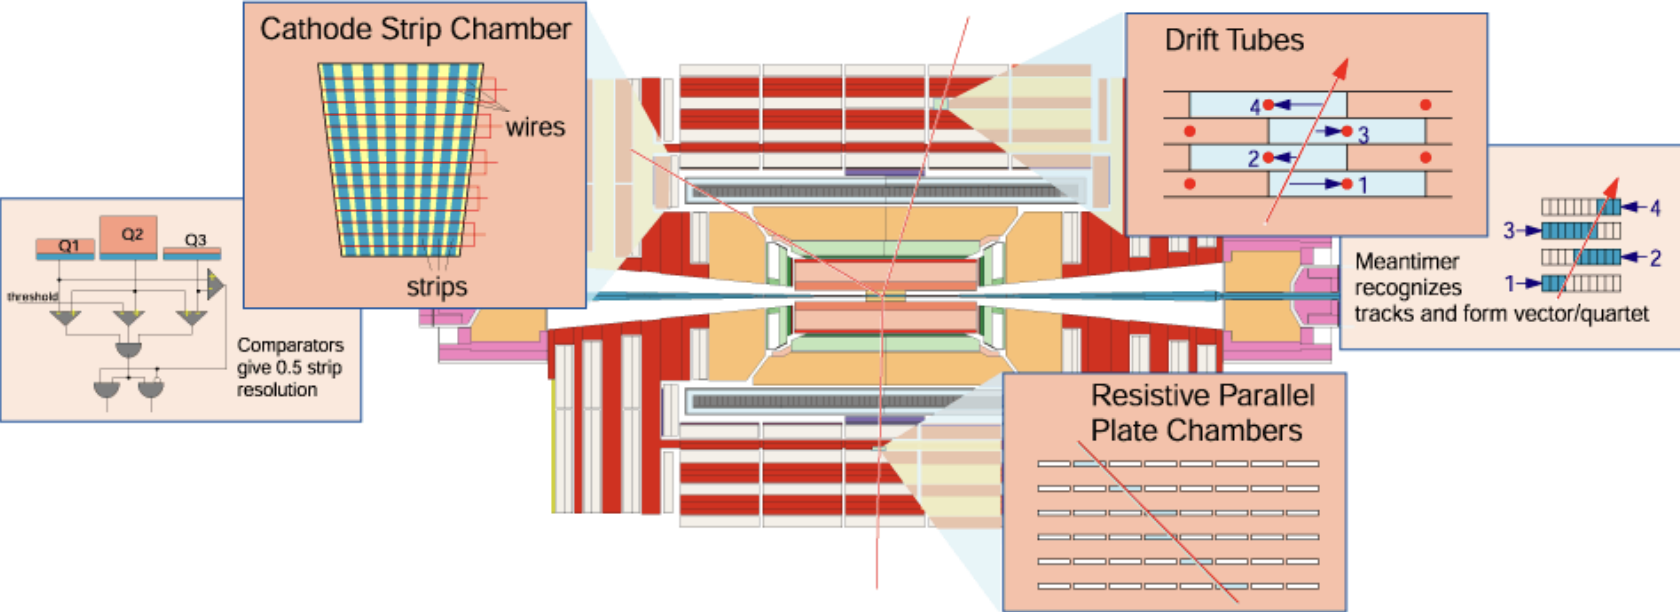
\includegraphics[width=0.8\textwidth]{muon_detector.png} % Replace with a Muon Detector diagram
    \caption{CMS Muon System layout, showing DTs, CSCs, and RPCs.}
    \label{fig:muon_detector}
\end{figure}

The muon system achieves momentum resolution of $\Delta p / p \sim 10\%$ at $1~\mathrm{TeV/c}$, contributing significantly to global track reconstruction.\cite{cms_tdr_muon}

\subsection{Trigger and Reconstruction}
The CMS trigger system is essential for managing the vast amount of data generated by the detector, selecting only the most relevant events for further analysis. The trigger operates in two levels: the Level-1 Trigger and the High-Level Trigger (HLT).

\subsection{Level-1 Trigger}
The Level-1 Trigger is a hardware-based system designed to process data in real time and reduce the event rate from 40 MHz to approximately 100 kHz \cite{trigger_tdr}. It uses custom electronics located close to the detector to analyze data from the calorimeters and muon chambers. This system identifies candidate particles such as muons, electrons, and jets, and makes decisions within microseconds.

The Level-1 Trigger ensures that only events with significant physics potential, such as those involving high-energy muons or missing transverse energy, are passed on to the next stage \cite{trigger_tdr}.

\subsection{High-Level Trigger (HLT)}
The High-Level Trigger is a software-based system that further reduces the event rate from 100 kHz to approximately 1 kHz, suitable for storage and offline analysis \cite{trigger_tdr}. The HLT uses a computing farm to reconstruct full events in real time, applying more sophisticated algorithms to refine the selection criteria.

This stage enables detailed analysis of particle trajectories and energy deposits, ensuring that only the most promising events are retained for later study. The combination of the Level-1 Trigger and HLT allows CMS to efficiently manage the enormous data flow while preserving the ability to capture rare and significant physics phenomena.


\section{Conclusion}
The CMS detector integrates advanced subsystems, including the tracker, calorimeters, and muon chambers, to provide comprehensive coverage and high precision. These capabilities enable CMS to explore the rich physics opportunities at the LHC.


% % Chapter 3. Dataset
\chapter{Dataset}
\section{Geant4 Simulation}

Geant4 is a powerful and widely used simulation toolkit for modeling the passage of particles through matter. It provides detailed simulations of detector geometry, material interactions, and physics processes, enabling accurate predictions of detector responses. In the context of the CMS detector, Geant4 plays a critical role in validating experimental results and designing upgrades like the HGCal.

\subsection{Physics Processes}

Geant4 includes a comprehensive suite of physics processes covering electromagnetic, hadronic, and optical interactions. For the HGCal, electromagnetic processes such as ionization, bremsstrahlung, and photon interactions are particularly important in the CE-E section, while hadronic processes are crucial for modeling particle showers in the CE-H \cite{geant4_toolkit}.

\subsection{Geometry and Materials}

Geant4 enables users to define complex and highly detailed detector geometries with exceptional precision and flexibility. Taking the High-Granularity Calorimeter (HGCal) as an example, the arrangement of silicon sensors, scintillator tiles, and absorber plates is accurately modeled in Geant4. Each component is defined in terms of its precise geometry and physical properties, including parameters such as density, radiation length, and interaction cross-sections.

Through Geant4, the HGCal geometry is meticulously constructed layer by layer. Silicon sensors, segmented into hexagonal cells, simulate active regions where particles interact to generate measurable signals. Absorber materials like lead and steel are defined to induce particle showers, while scintillator tiles are incorporated to detect the resulting secondary particles. This level of detail ensures that simulations replicate real-world interactions, providing reliable data for performance optimization and physics studies.

\subsection{Applications in HGCal Development}

Geant4 has been instrumental in optimizing the design of the HGCal. By simulating different configurations and material choices, researchers have fine-tuned the detector to achieve the desired performance in terms of energy resolution, granularity, and radiation tolerance. These simulations also help in developing reconstruction algorithms and calibrations tailored to the unique characteristics of the HGCal \cite{geant4_toolkit}.

\begin{figure}[h]
    \centering
    %\includegraphics[width=\textwidth]{Geant4_Simulation.png}
    \caption{Visualization of a Geant4 simulation for the HGCal, showing particle showers in the calorimeter layers. (Image credit: Geant4 Collaboration)}
    \label{fig:geant4_simulation}
\end{figure}

Geant4 remains an indispensable tool in the development and operation of the CMS detector, enabling detailed studies of particle interactions and supporting advancements in high-energy physics.

\section{The Fast Calorimeter Simulation Challenge (CaloChallenge)}

The Fast Calorimeter Simulation Challenge, or CaloChallenge, is an initiative designed to advance the development of fast, accurate, and efficient generative models for calorimeter shower simulations. This challenge bridges the gap between traditional simulation methods like GEANT4 and novel machine learning approaches, providing datasets, benchmarks, and metrics for evaluation \cite{calochallenge}.

\subsection{Objectives}

CaloChallenge has the following primary goals:

\begin{itemize}
    \item Encourage the development of generative models capable of fast and accurate calorimeter shower simulation.
    \item Provide standardized datasets and metrics for consistent evaluation and benchmarking.
    \item Foster collaboration across the high-energy physics and machine learning communities.
\end{itemize}

\subsection{Datasets}

The CaloChallenge offers three distinct datasets, each increasing in complexity, to evaluate model performance in diverse scenarios. The datasets are as follows:

\subsubsection{Dataset 1: ATLAS GEANT4 Open Datasets}
Dataset 1 is based on simulations using the ATLAS detector geometry. It includes two particle types: photons and charged pions. The voxelized shower information is derived from single particles produced at the calorimeter surface in the $\eta$ range of 0.2-0.25. The detector geometry consists of 5 layers for photons and 7 layers for pions, with the number of radial and angular bins varying by layer and particle type. This results in 368 voxels for photons and 533 voxels for pions.

The dataset spans 15 discrete incident energy levels, ranging from 256 MeV to 4 TeV in powers of two. Each energy level contains 10k events, except for the higher energies, where fewer events are available due to statistical limitations. This dataset serves as a benchmark for evaluating generative models on simpler detector geometries and energy distributions.

\subsubsection{Dataset 2: Multi-Layer Geometry with Electrons}
Dataset 2 focuses on simulations of electrons interacting with a concentric cylindrical detector geometry. The detector comprises 45 layers, each with both active (silicon) and passive (tungsten) material. Each layer is divided into 9 radial bins and 16 angular bins, resulting in a total of 6480 voxels (45 $\times$ 16 $\times$ 9). 

The electron energies are sampled from a log-uniform distribution ranging from 1 GeV to 1 TeV, offering a continuous spectrum of energy levels. The dataset contains 100k events, enabling models to explore and learn intricate energy depositions across the detector geometry. This dataset challenges models to handle the complexities of high-granularity detectors.

\subsubsection{Dataset 3: High-Granularity Calorimeter Geometry}
Dataset 3 simulates a high-granularity calorimeter with an advanced detector geometry. Like Dataset 2, it features 45 layers with active (silicon) and passive (tungsten) material. However, the granularity is significantly higher, with each layer containing 18 radial bins and 50 angular bins. This results in a total of 40,500 voxels (45 $\times$ 50 $\times$ 18).

The dataset consists of electron showers with energies sampled from a log-uniform distribution ranging from 1 GeV to 1 TeV. Each file contains 50k events, offering robust training and evaluation datasets. This dataset is designed to test models' ability to generalize and simulate realistic particle physics scenarios with highly detailed detector geometries.


\subsection{Data Format}

Each dataset is stored as one or more HDF5 files created using Python's \texttt{h5py} module with gzip compression. The files include:

\begin{itemize}
    \item \texttt{incident\_energies}: An array of shape (\texttt{num\_events}, 1) containing the incoming particle energies in MeV.
    \item \texttt{showers}: An array of shape (\texttt{num\_events}, \texttt{num\_voxels}) storing the energy depositions (in MeV) for each voxel, flattened in a specific order.
\end{itemize}

The mapping of voxel indices to spatial coordinates follows the detector segmentation. Helper functions are provided for reshaping and handling the data.

\subsection{Evaluation Metrics}

CaloChallenge evaluates the generative models using multiple metrics, including:

\begin{itemize}
    \item A binary classifier trained to distinguish between real GEANT4 samples and model-generated samples.
    \item Chi-squared comparisons between histograms of high-level features, such as layer energies and shower shapes.
    \item Speed and resource usage metrics, such as training time, generation time, and memory footprint.
    \item Interpolation capabilities to test generalization across unseen particle energies.
\end{itemize}

\subsection{Community Engagement}

Participants are encouraged to share their findings and contribute to community discussions. The challenge concludes with a workshop to present results, compare approaches, and collaborate on a community paper documenting the outcomes. For communication and updates, participants can join the ML4Jets Slack channel and the Google Groups mailing list \cite{calochallenge}.

For further details, visit the official CaloChallenge GitHub repository: \url{https://github.com/CaloChallenge/homepage}.






% % Chapter 4. Algorithm
\chapter{Algorithm}
\section{Score-based Diffusion Model}
Before diffusion models were introduced, generative models were primarily based on Variational Autoencoders (VAEs) and Generative Adversarial Networks (GANs). While VAEs are effective for compressing data, they struggle to generate high-quality, diverse samples due to their reliance on sampling from a normal distribution in the latent space. GANs, on the other hand, have demonstrated success in generating realistic samples but can be challenging to train and prone to mode collapse.

One drawback of Variational Autoencoders (VAEs) is the inclusion of the KL divergence term in their loss function. While VAEs are effective for compressing data (encoding), they struggle to generate high-quality, diverse samples. This limitation stems from their reliance on sampling from a normal distribution in the latent space. Although VAEs are trained to bring the posterior distribution close to a Gaussian, in practice, the match is often not precise enough to ensure that samples drawn from this distribution will be of high quality.

Therefore, an alternative approach, introduced in 2015, is the “diffusion model,” which can be implemented using either score-matching or denoising techniques. Diffusion models aim to generate synthetic data based on a set of independent, identically distributed (i.i.d.) samples drawn from an unknown data distribution. The key concept is to simulate new samples by either employing denoising Score Langevin Dynamics (SMLD) or implementing Denoising Diffusion Probabilistic Model (DDPM), where a deep neural network approximates the score, or gradient, of the log-density of the data distribution. Next we will discuss the two methods in detail.

\subsection{Denoising Score Matching with Langevin Dynamics (SMLD)}
Langevin Dynamics in generative modeling is a way to generate samples by simulating a process that gradually moves from random points in space toward areas with high probability density, where most of the real data is located. It does this by changing along the directions defined by the gradient of the probability distribution, called the "score" in our context. At each step, a small amount of Gaussian noise is added to introduce randomness, ensuring that each path taken is unique and prevents the sampling process from getting "stuck" in local regions.

In simpler terms, think of Langevin Dynamics as a guided walk starting from a random spot and following a path that gradually leads toward more typical or likely values of the data (like images, text, etc.). The direction of each step is influenced by both the data structure (moving toward areas where data is dense) and a bit of noise to keep things varied, which helps to explore the whole space more effectively. This makes Langevin Dynamics an effective sampling method for creating new data points in generative modeling.

In this approach, we define a perturbation mechanism \( p_\sigma(\tilde{x} | x) = \mathcal{N}(\tilde{x}; x, \sigma^2 I) \), which acts as a Gaussian kernel centered at \( x \) with variance \( \sigma^2 \). This perturbation is integrated over the data distribution \( p_{\text{data}}(x) \) to yield the broader distribution \( p_\sigma(\tilde{x}) = \int p_{\text{data}}(x) p_\sigma(\tilde{x} | x) \, dx \). 

We consider a range of increasing noise scales, where \( \sigma_{\min} = \sigma_1 < \sigma_2 < \dots < \sigma_N = \sigma_{\max} \). Typically, \( \sigma_{\min} \) is chosen to be small enough that \( p_{\sigma_{\min}}(x) \approx p_{\text{data}}(x) \), capturing the original data distribution, while \( \sigma_{\max} \) is set large enough so that \( p_{\sigma_{\max}}(x) \approx \mathcal{N}(x; 0, \sigma_{\max}^2 I) \), resembling a Gaussian prior.

Following the work of Song and Ermon \cite{song_generative_2020}, we train a Noise Conditional Score Network (NCSN), denoted \( s_\theta(x, \sigma) \), by minimizing a weighted sum of denoising score matching objectives as follows:

\begin{equation}
\theta^* = \arg \min_{\theta} \sum_{i=1}^{N} \sigma_i^2 \, \mathbb{E}_{p_{\text{data}}(x)} \, \mathbb{E}_{p_{\sigma_i}(\tilde{x} | x)} \left[ \| s_\theta(\tilde{x}, \sigma_i) - \nabla_{\tilde{x}} \log p_{\sigma_i}(\tilde{x} | x) \|_2^2 \right].
\end{equation}

Given sufficient data and model capacity, the resulting score-based model \( s_\theta^*(x, \sigma) \) estimates the gradient \( \nabla_x \log p_{\sigma}(x) \) across noise scales \( \sigma \in \{\sigma_i\}_{i=1}^{N} \).

So the Langevin Dynamics process can be described as follows:

\begin{equation}
\mathbf{x}_i = \mathbf{x}_{i-1} + \sqrt{\sigma_{i}^2 - \sigma_{i-1}^2} \mathbf{z}_{i-1} , i = 1, 2, \dots, N
\end{equation}



\subsection{ Denoising Diffusion Probabilistic Model (DDPM)}
Next, we are going to introduce the second method for diffusing models, the Denoising Diffusion Probabilistic Model (DDPM)~\cite{DDPM_2020}. Unlike SMLD, DDPM incorporates a scaling factor for \( x \), which modifies the approach slightly. The basic idea is to define the conditional probability distribution as follows: \( p(x_i | x_{i-1}) = \mathcal{N} \left( x_i ; \sqrt{1 - \beta_i} x_{i-1}, \beta_i I \right) \).

Following Sohl-Dickstein et al.~\cite{Dickstein2015} and Ho et al.~\cite{DDPM_2020}, let us consider a set of positive noise scales \( 0 < \beta_1, \beta_2, \dots, \beta_N < 1 \). For each data point \( x_0 \sim p_{\text{data}}(x) \), we define a discrete Markov chain \( \{x_0, x_1, \dots, x_N\} \), with each transition given by \( p(x_i | x_{i-1}) = \mathcal{N} \left( x_i ; \sqrt{1 - \beta_i} x_{i-1}, \beta_i I \right) \). Consequently, we can write the marginal distribution \( p_{\alpha_i}(x_i | x_0) = \mathcal{N} \left( x_i ; \sqrt{\alpha_i} x_0, (1 - \alpha_i) I \right) \), where \( \alpha_i := \prod_{j=1}^i (1 - \beta_j) \).

As in SMLD, we also train it by minimizing the denoising score matching objective:

\begin{equation}
\theta^* = \arg \min_{\theta} \sum_{i=1}^{N} (1-\alpha_i) \, \mathbb{E}_{p_{\text{data}}(x)} \, \mathbb{E}_{p_{\alpha_i}(\tilde{x} | x)} \left[ \| s_\theta(\tilde{x}, \alpha_i) - \nabla_{\tilde{x}} \log p_{\alpha_i}(\tilde{x} | x) \|_2^2 \right].
\end{equation}

where again, $1-\alpha_i$ is just a weighting factor.

What's more, we can define the perturbed data distribution as \( p_{\alpha_i}(\tilde{x}) := \int p_{\text{data}}(x) p_{\alpha_i}(\tilde{x} | x) dx \). The noise scales are chosen so that \( x_N \) approximates a standard normal distribution \( \mathcal{N}(0, I) \). So the simialr form as SMLD will be 

\begin{equation}
    x_{t-1} = \sqrt{1 - \beta_t} x_t + \sqrt{\beta_t} z_t, \quad t = N, N-1, \dots, 1  
\end{equation}

where \( z_t \sim \mathcal{N}(0, I) \) are standard normal samples. The final sample \( x_0 \) is drawn from the data distribution \( p_{\text{data}}(x) \). The process is repeated for each data point, and the final samples are generated by running the Markov chain for \( T \) steps. The resulting samples are expected to approximate the data distribution \( p_{\text{data}}(x) \) when \( T \to \infty \) under suitable conditions.
\section{Forward Process}
So far, we have discussed two ways of simulating new samples from a given data distribution. Although they look different, both methods are based on the same principle: iteratively transforming a sample from a simple distribution (e.g., a Gaussian) to a more complex one (e.g., the data distribution). 

Based on the work of Yang Song \cite{song_generative_2020}, we can generalize this concept through what is called the \textbf{forward process} in diffusion models.

Our goal is to construct a diffusion process \( x_{t} \) indexed by a continuous time variable \( t \in [0, T] \), such that:
\begin{equation}
    x_{0} \sim p_{0}
\end{equation}
for which we have a dataset of independent and identically distributed (i.i.d.) samples, and
\begin{equation}
    x_{T} \sim p_{T}
\end{equation}
for which we have a tractable form to generate samples efficiently. In other words, \( p_{0} \) is the data distribution and \( p_{T} \) is the prior distribution.

This diffusion process can be modeled as the solution to an Itô stochastic differential equation (SDE):
\begin{equation}
    dx = f(x, t) \, dt + g(t) \, dw
\end{equation}
where:
\begin{itemize}
    \item \( x \) is the state variable,
    \item \( f(x, t) \) is the drift coefficient,
    \item \( g(t) \) is the diffusion coefficient,
    \item \( w \) is a Wiener process (Brownian motion).
\end{itemize}

For later we can show that this has a slightly better result than orginal DDPM and SMLD.



\section{Backward Process}

With the forward process established, we can now construct the \textbf{backward process}. The aim of this process is to generate samples from the data distribution \( p_{0} \), given samples from the prior distribution \( p_{T} \).

The continuous form of this process is defined by the following stochastic differential equation (SDE):

\begin{equation}
d\mathbf{x} = \mathbf{f}_t(\mathbf{x}) \, dt + g_t \, d\mathbf{w} \label{eq:sde-forward}
\end{equation}

To direclty prove the reverse SDE formula in continuous form will be a little complex. But we can get the same spirit from discrete form, as \( \Delta t \to 0 \), the continuous equation above can be approximated by:

\begin{equation}
\mathbf{x}_{t+\Delta t} - \mathbf{x}_t = \mathbf{f}_t(\mathbf{x}_t) \, \Delta t + g_t \sqrt{\Delta t} \, \mathbf{\varepsilon}, \quad \mathbf{\varepsilon} \sim \mathcal{N}(\mathbf{0}, \mathbf{I}) \label{eq:sde-discrete}
\end{equation}

The discrete form of the stochastic differential equation (SDE) is especially valuable for practical computer implementations. By breaking down the continuous process into discrete steps, we can simulate both the diffusion and reverse processes incrementally, allowing us to generate samples using numerical methods. This approach enables us to approximate continuous dynamics with a series of discrete updates, making the computations more manageable and efficient.

In this way, using the SDE framework to describe diffusion models provides a clear distinction between theoretical analysis and practical implementation. We can rely on the mathematical properties of continuous SDEs for analysis, while in actual applications, we have the flexibility to choose any appropriate discretization method for efficient numerical calculation.

In probabilistic terms, Equation \eqref{eq:sde-discrete} implies that the conditional probability is given by

\begin{equation}
\begin{aligned}
p(\mathbf{x}_{t+\Delta t}|\mathbf{x}_t) =&\, \mathcal{N}\left(\mathbf{x}_{t+\Delta t}; \mathbf{x}_t + \mathbf{f}_t(\mathbf{x}_t) \, \Delta t, g_t^2 \, \Delta t \, \mathbf{I}\right) \\
\propto&\, \exp\left(-\frac{\|\mathbf{x}_{t+\Delta t} - \mathbf{x}_t - \mathbf{f}_t(\mathbf{x}_t) \, \Delta t\|^2}{2 g_t^2 \Delta t}\right)
\end{aligned} \label{eq:sde-proba}
\end{equation}

Now since our goal is to use the forward process to derive the backward process, which means obtaining \( p(\mathbf{x}_t|\mathbf{x}_{t+\Delta t}) \), we apply Bayes' theorem, as shown in "A Discussion on Generative Diffusion Models: DDPM = Bayesian + Denoising":~\cite{noauthor_ddpm_nodate}

\begin{equation}
\begin{aligned}
p(\mathbf{x}_t|\mathbf{x}_{t+\Delta t}) =&\, \frac{p(\mathbf{x}_{t+\Delta t}|\mathbf{x}_t) p(\mathbf{x}_t)}{p(\mathbf{x}_{t+\Delta t})} \\
=&\, p(\mathbf{x}_{t+\Delta t}|\mathbf{x}_t) \exp\left(\log p(\mathbf{x}_t) - \log p(\mathbf{x}_{t+\Delta t})\right) \\
\propto&\, \exp\left(-\frac{\|\mathbf{x}_{t+\Delta t} - \mathbf{x}_t - \mathbf{f}_t(\mathbf{x}_t) \Delta t\|^2}{2 g_t^2 \Delta t} + \log p(\mathbf{x}_t) - \log p(\mathbf{x}_{t+\Delta t})\right)
\end{aligned} \label{eq:bayes-dt}
\end{equation}

It is not difficult to see that when \( \Delta t \) is sufficiently small, \( p(\mathbf{x}_{t+\Delta t}|\mathbf{x}_t) \) will be significantly non-zero only when \( \mathbf{x}_{t+\Delta t} \) is close to \( \mathbf{x}_t \). Conversely, only in this case will \( p(\mathbf{x}_t|\mathbf{x}_{t+\Delta t}) \) be significantly non-zero. Therefore, we only need to conduct an approximate analysis for situations where \( \mathbf{x}_{t+\Delta t} \) is close to \( \mathbf{x}_t \). For this, we can use a Taylor expansion:

\begin{equation}
\log p(\mathbf{x}_{t+\Delta t}) \approx \log p(\mathbf{x}_t) + (\mathbf{x}_{t+\Delta t} - \mathbf{x}_t) \cdot \nabla_{\mathbf{x}_t} \log p(\mathbf{x}_t) + \Delta t \, \frac{\partial}{\partial t} \log p(\mathbf{x}_t)
\end{equation}

It is important not to neglect the term \( \frac{\partial}{\partial t} \), because \( p(\mathbf{x}_t) \) is a function of both \( t \) and \( \mathbf{x}_t \), while \( p(\mathbf{x}_{t+\Delta t}) \) is a function of \( t + \Delta t \) and \( \mathbf{x}_{t+\Delta t} \). Thus, \( p(\mathbf{x}_t) \) must include an additional time derivative. Substituting this into Equation \eqref{eq:bayes-dt} allows us to derive:

\begin{equation}
p(\mathbf{x}_t|\mathbf{x}_{t+\Delta t}) \propto \exp\left(-\frac{\|\mathbf{x}_{t+\Delta t} - \mathbf{x}_t - \left[\mathbf{f}_t(\mathbf{x}_t) - g_t^2 \nabla_{\mathbf{x}_t} \log p(\mathbf{x}_t) \right] \Delta t\|^2}{2 g_t^2 \Delta t} + \mathcal{O}(\Delta t)\right)
\end{equation}

As \( \Delta t \to 0 \), the term \( \mathcal{O}(\Delta t) \) becomes negligible, thus:

\begin{equation}
\begin{aligned}
p(\mathbf{x}_t|\mathbf{x}_{t+\Delta t}) \propto&\, \exp\left(-\frac{\|\mathbf{x}_{t+\Delta t} - \mathbf{x}_t - \left[\mathbf{f}_t(\mathbf{x}_t) - g_t^2 \nabla_{\mathbf{x}_t} \log p(\mathbf{x}_t) \right] \Delta t\|^2}{2 g_t^2 \Delta t}\right)
\end{aligned}
\end{equation}

Finally, the above formula indicates that the reverse process also contains a deterministic part and a stochastic part. The deterministic part consists of \( \mathbf{f}_t(\mathbf{x}_t) - g_t^2 \nabla_{\mathbf{x}_t} \log p(\mathbf{x}_t) \), while the stochastic part is \( g_t \sqrt{\Delta t} \mathbf{\varepsilon} \).

Thus, our reverse process is defined as:
\begin{equation}
\mathbf{x}_{t-\Delta t} = \mathbf{x}_t - \left[\mathbf{f}_t(\mathbf{x}_t) - g_t^2 \nabla_{\mathbf{x}_t} \log p(\mathbf{x}_t) \right] \Delta t + g_t \sqrt{\Delta t} \mathbf{\varepsilon} \label{eq:reverse}
\end{equation}

We can use the picture below to illustrate the forward and backward processes in a diffusion model:

\begin{figure}[ht]
    \centering
    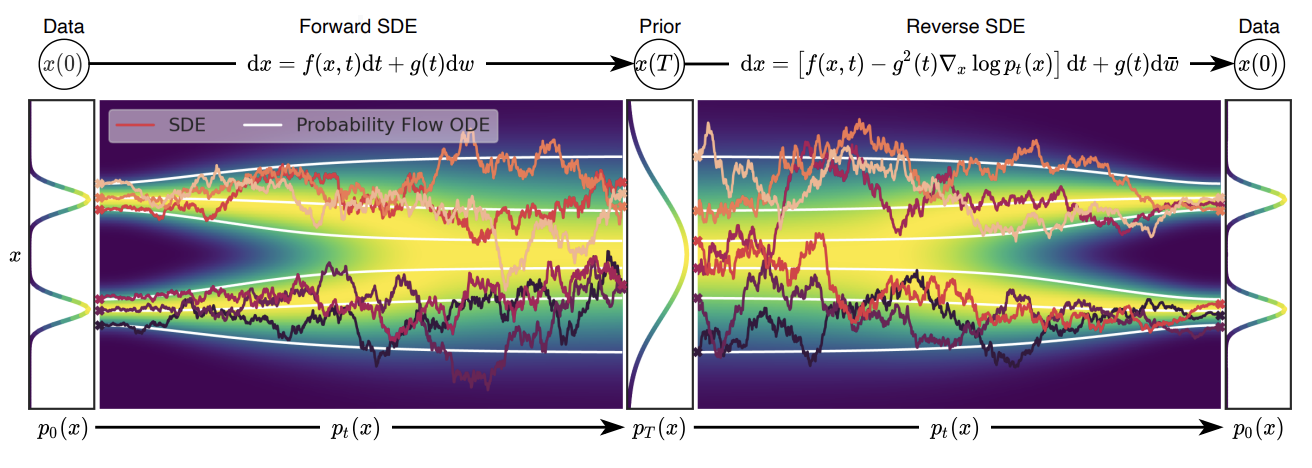
\includegraphics[width=0.8\textwidth]{Figures/diffusion.png}
    \caption{Forward and Backward Processes in Diffusion Models (The picture is from Song and Ermon (2019))}
    \label{fig:forward-backward}
\end{figure}

\section{VE, VP SDEs}

\subsection{Continuos Forward Process}
After we established the general form of the forward and backward processes, we can now go back to see how to apply them on SMLD (VE mthoed) and DDPM (VP method).

So in this section, we try to present detailed derivations demonstrating that the noise perturbations in SMLD (Score-based generative modeling via Langevin Dynamics) and DDPM (Denoising Diffusion Probabilistic Models) are discretizations of the Variance Exploding (VE) and Variance Preserving (VP) Stochastic Differential Equations (SDEs), respectively. 

First, when utilizing a total of \( N \) noise scales, each perturbation kernel \( p_{\sigma_i}(x | x_0) \) for SMLD can be derived from the following Markov chain:

\begin{equation}
x_i = x_{i-1} + \sqrt{\sigma_i^2 - \sigma_{i-1}^2} z_{i-1}, \quad i = 1, 2, \ldots, N,
\end{equation}

\noindent
where \( z_{i-1} \sim \mathcal{N}(0, I) \) and \( x_0 \sim p_{\text{data}} \). Here, we introduce \( \sigma_0 = 0 \) for simplicity. As \( N \to \infty \), the Markov chain \( \{ x_i \}_{i=1}^N \) converges to a continuous stochastic process \( \{ x(t) \}_{t=0}^1 \), and \( \{ \sigma_i \}_{i=1}^N \) becomes a function \( \sigma(t) \), while \( z_i \) transitions to \( z(t) \). We denote the continuous time variable as \( t \in [0, 1] \) instead of the integer index \( i \in \{ 1, 2, \ldots, N \} \). Let $\mathbf{x} ( \frac{i}{N} ) = \mathbf{x}_i$, $\mathbf{\sigma} ( \frac{i}{N} ) = \mathbf{\sigma}_i$, $\mathbf{z} ( \frac{i}{N} ) = \mathbf{z}_i$, for $i = 1, 2, \ldots, N$. 
Rewriting Equation \refeq{eq:ddpm-discrete} with $\Delta t = \frac{1}{N}$ gives:
 
\begin{equation}
x(t + \Delta t) = x(t) + \sqrt{\sigma^2(t + \Delta t) - \sigma^2(t)} z(t) \approx x(t) + \sqrt{\frac{d \sigma^2(t)}{dt}} \Delta t z(t),
\end{equation}

\noindent
where the approximation holds as \( \Delta t \to 0 \). In the limit of \( \Delta t \to 0 \), we obtain the VE SDE:

\begin{equation}
dx = \sqrt{\frac{d \sigma^2(t)}{dt}} dw.
\end{equation}

\noindent
Furthermore, we usually let $\sigma$ sequence to be a geometric sequence. We have $\sigma (\frac{i}{N}) = \sigma_i = \sigma_{\min} (\frac{\sigma_{\max}}{\sigma_{\min}})^{\frac{i-1}{N-1}}$ for i ranges from 1 to N. If \( N \to \infty \)

\noindent
The corresponding VE SDE is 

\begin{equation}
    d \mathbf{x} = \sigma_{\min} \left( \frac{\sigma_{\max}}{\sigma_{\min}} \right) ^t \sqrt{2 \log \left( \frac{\sigma_{\max}}{\sigma_{\min}} \right) } \, d \mathbf{w}, \quad t \in (0, 1).
\end{equation}

\noindent
For the perturbation kernels \( p_{\alpha_i}(x | x_0) \) used in DDPM, the discrete Markov chain is given by:

\begin{equation}
\mathbf{x}_i = \sqrt{1 - \beta_i} \mathbf{x}_{i-1} + \sqrt{1 - \beta_i} z_{i-1}, \quad i = 1, 2, \ldots, N \label{eq:ddpm-discrete}
\end{equation}

\noindent
where \( z_{i-1} \sim \mathcal{N}(0, I) \). To obtain the limit of this Markov chain as \( N \to \infty \), we define an auxiliary set of noise scales \( \{ \bar{\beta}_i \}_{i=1}^N \) and rewrite Equation \refeq{eq:ddpm-discrete} as follows:

\begin{equation}
\mathbf{x}_i = \sqrt{1 - \bar{\beta}_i} \mathbf{x}_{i-1} + \sqrt{1 - \bar{\beta}_i} z_{i-1}, \quad i = 1, 2, \ldots, N \label{eq:ddpm-discrete}
\end{equation}

\noindent
As \( N \to \infty \), the noise scales \( \{ \bar{\beta}_i \}_{i=1}^N \) converge to a function \( \beta(t) \) indexed by \( t \in [0, 1] \). Let \( \{ \bar{\beta}_i \}_{N} = \beta \) and \( \{ x_i \}_{N} = x \) and \( \{ z_i \}_{N} = z \). Rewriting Equation \refeq{eq:vp-sde} gives:

\begin{equation}
\begin{aligned}
    \mathbf{x}(t + \Delta t) &= \sqrt{1 - \beta(t + \Delta t)} \mathbf{x}(t) + \sqrt{1 - \beta(t + \Delta t)} z(t) \\ &\approx \mathbf{x}(t) -\frac{1}{2}\beta(t + \Delta t) \Delta t \mathbf{x}(t)+\sqrt{\beta(t + \Delta t) \Delta t } \mathbf{z} (t) \\
    &\approx \mathbf{x}(t) -\frac{1}{2}\beta(t ) \Delta t \mathbf{x}(t)+\sqrt{\beta(t ) \Delta t } \mathbf{z} (t) 
\end{aligned} \label{eq:ddpm-discrete}
\end{equation}

\noindent
where the approximation holds as \( \Delta t \to 0 \). Therefore, in the limit of \( \Delta t \to 0 \), we obtain the VP SDE:

\begin{equation}
d \mathbf{x} = -\frac{1}{2} \beta(t) \mathbf{x} \, dt + \sqrt{\beta(t)} \, d\mathbf{w}.\label{eq:vp-sde}
\end{equation}

\noindent
As in DDPM, $\beta$ is typically an arithmetic sequence where $\beta_i = \beta_{\min} + t (\beta_{\max} - \beta_{\min}) $ for t ranges from 0 to 1 if \( N \to \infty \). This will then give us the VP SDE as

\begin{equation}
    d \mathbf{x} = -\frac{1}{2} \left( \beta_{\min} + t (\beta_{\max} - \beta_{\min} )\right) \mathbf{x} \, dt + \sqrt{\beta_{\min} + t (\beta_{\max} - \beta_{\min})} \, d\mathbf{w}, \quad t \in (0, 1).
\end{equation}

\noindent
In conclusion, the contents above indicate that 

\noindent
For SMLD (Variance Exploding SDE - VE):
\begin{itemize}
    \item \( f(x, t) = 0 \)
    \item \( g(t) = \sigma_{\min} \left( \frac{\sigma_{\max}}{\sigma_{\min}} \right)^t \sqrt{2 \log \left( \frac{\sigma_{\max}}{\sigma_{\min}} \right)} \)
\end{itemize}

\vspace{1em}

\noindent
For DDPM (Variance Preserving SDE - VP):
\begin{itemize}
    \item \( f(x, t) = -\frac{1}{2} \beta(t) x \)
    \item \( g(t) = \sqrt{\beta(t)} \)
\end{itemize}

\subsection{Continuos Backward Process - PC Sampler}

Here we can of course use the $f(x,t)$ and $g(t)$ to do the reverse process as equation \eqref{eq:reverse} shows. However, here we possess additional insights that can enhance our solution methods. Specifically, with our score-based model 
$s_{\theta^*}(x, t) \approx \nabla_x \log p_t(x)
$, we can utilize score-based Markov Chain Monte Carlo (MCMC) techniques to sample directly from the distribution $p_t$ and refine the outputs of a numerical SDE solver.

At each time step, the numerical SDE solver provides an initial estimate for the sample at the next time step, functioning as a "predictor." Subsequently, the score-based MCMC method adjusts the estimated sample's marginal distribution, acting as a "corrector." This approach is reminiscent of Predictor-Corrector methods. We similarly refer to our hybrid sampling algorithms as Predictor-Corrector (PC) samplers.

The PC samplers extend the original sampling methodologies of SMLD and DDPM: the SMLD method employs an identity function as the predictor and utilizes annealed Langevin dynamics as the corrector. In contrast, the DDPM method adopts ancestral sampling as the predictor and the identity function as the corrector.

\noindent\textbf{Algorithm 1} \textit{PC sampling (VE SDE)}
\begin{algorithmic}[1]
    \STATE $\mathbf{x}_N \sim \mathcal{N}(0, \sigma_{\max}^2 \mathbf{I})$
    \FOR{$i = N - 1$ to $0$}
        \STATE $\mathbf{x}'_i = \mathbf{x}_i -g^2(t)s_\theta^* \left( \mathbf{x}_i, \sigma_i \right) {\Delta t}$
        \STATE $\mathbf{z} \sim \mathcal{N}(0, \mathbf{I})$
        \STATE $\mathbf{x}_i = \mathbf{x}'_i +g(t) \sqrt{\Delta t} \mathbf{z}$
        \FOR{$j = 1$ to $M$}
            \STATE $\mathbf{z} \sim \mathcal{N}(0, \mathbf{I})$
            \STATE $\mathbf{x}_i \leftarrow \mathbf{x}_i + \epsilon_i s_\theta^* \left( \mathbf{x}_i, \sigma_i \right) + \sqrt{2 \epsilon_i} \mathbf{z}$
        \ENDFOR
    \ENDFOR
    \RETURN $\mathbf{x}_0$
\end{algorithmic}

\bigskip

\noindent\textbf{Algorithm 2} \textit{PC sampling (VP SDE)}
\begin{algorithmic}[1]
    \STATE $\mathbf{x}_N \sim \mathcal{N}(0, \mathbf{I})$
    \FOR{$i = N - 1$ to $0$}
        \STATE $\mathbf{x}'_i = (f(x,t)-g^2(t)*s_\theta^* \left( \mathbf{x}_{i+1}, i+1 \right)) {\Delta t}$
        \STATE $\mathbf{z} \sim \mathcal{N}(0, \mathbf{I})$
        \STATE $\mathbf{x}_i = \mathbf{x}'_i +g(t) \sqrt{\Delta t} \mathbf{z}$
        \FOR{$j = 1$ to $M$}
            \STATE $\mathbf{z} \sim \mathcal{N}(0, \mathbf{I})$
            \STATE $\mathbf{x}_i \leftarrow \mathbf{x}_i + \epsilon_i s_\theta^* \left( \mathbf{x}_i, i \right) + \sqrt{2 \epsilon_i} \mathbf{z}$
        \ENDFOR
    \ENDFOR
    \RETURN $\mathbf{x}_0$
\end{algorithmic}

where $\epsilon$ is defined as 

\begin{equation}
    \epsilon = 2 r^2 \frac{\|\mathbf{z}\|_2^2}{\|s_\theta\|_2^2}
\end{equation}

and $r$ is a hyperparameter that controls the step size of the Langevin dynamics.









% % Chapter 5. Model Structure
\chapter{Model Structure}

In the previous chapter, we introduced the foundational algorithms employed in this research project. This chapter delves into the structure of our custom Transformer-based model, designed to predict the "score" or gradient in detector simulations. Built upon the Transformer architecture—a cutting-edge model in deep learning—our model incorporates several modifications to enhance its applicability in high-energy physics detector simulations.

We chose the Transformer architecture not only for its power and versatility but also for its unique suitability for data with rotational invariance. In our research, each input consists of multiple showers, each shower containing several hits, and each hit represented by four features, as introduced in Chapter 3. This structure makes our data rotationally invariant, meaning that the relationships within the data remain consistent even if the order of hits within a shower or the showers within an input are rearranged. Transformers are particularly well-suited for handling such properties. Their self-attention mechanism enables them to learn and capture relationships between data points in a way that is invariant to transformations like rotation. This flexibility is especially advantageous for our detector simulations, where capturing invariant relationships is crucial for making accurate predictions.

We will begin by exploring the evolution of Transformers from Recurrent Neural Networks (RNNs), highlighting how Transformer architectures overcame the limitations of sequential models. Following this, we will examine the core components of the Transformer model, including its different architectural types (encoder-only, decoder-only, and encoder-decoder models) and the self-attention mechanism, which lies at the heart of the Transformer’s ability to model long-range dependencies.

After establishing an understanding of the original Transformer architecture, we will discuss the custom modifications introduced in our model to optimize it for detector simulations. Key innovations include the \textbf{Gaussian Fourier Projection} for encoding temporal information, which allows the model to capture high-frequency dependencies by transforming time and incident energy into sinusoidal features. Additionally, we introduce a specialized \textbf{mean-field attention mechanism}, a variant of self-attention tailored to efficiently aggregate global context. Mean-field attention leverages a class token to summarize information across the sequence, reducing computational complexity while retaining essential global information.

Furthermore, our model incorporates residual network structures and layer normalization to stabilize and expedite the training process. We will explain how these modifications, along with our encoder-only architecture, facilitate efficient information flow, enabling the model to focus on capturing the relationships within the data rather than generating sequences. We also employ \textbf{Weights \& Biases (wandb)} for parameter tuning, using its sweep functionality to systematically explore hyperparameters such as the number of encoder blocks, attention heads, and dropout rates to achieve optimal performance.

In summary, this chapter provides a comprehensive overview of our custom Transformer model, from its foundational components to the innovative adjustments that make it well-suited for high-energy physics applications. Through these design choices, our model efficiently captures both local and global dependencies, thereby enhancing the accuracy and fidelity of detector simulations.

\section{Transformer}

\subsection{Introduction}

Transformer models have revolutionized deep learning by enabling efficient and scalable processing of sequential and structured data. Originally introduced for natural language processing, Transformers have since demonstrated remarkable versatility across various domains, including computer vision, time-series analysis, and scientific computing. Unlike traditional sequence models such as Recurrent Neural Networks (RNNs), which process data sequentially, Transformers utilize a self-attention mechanism that allows for parallel computation and long-range dependencies.

In high-energy physics, where data from particle detectors is vast, multidimensional, and often exhibits complex dependencies, Transformers provide significant advantages in both accuracy and efficiency. Their ability to capture intricate relationships between detector hits without being constrained by sequential processing makes them particularly suitable for simulations of particle showers, energy depositions, and collision dynamics. In the next section, we will explore the evolution from RNNs to Transformers, highlighting the limitations of sequential models and how Transformers address these challenges.

\subsection{The Evolution from RNNs to Transformers}

Figure \ref{fig:comparison} illustrates the fundamental differences in how RNNs and Transformers process sequential data. In the RNN model (A), the sequence is processed step by step, meaning that each input token $x_0$ is first passed into an RNN unit, which updates its internal state before moving to the next token $x_1$. At each step, the model relies on the hidden state from the previous timestep, which acts as a summary of all prior inputs. This recurrent dependency means that information flows sequentially through the network, making it impossible to process all tokens simultaneously. Instead, the model must first process $x_0$, then $x_1$, followed by $x_2$, and so on until $x_t$.

This sequential nature introduces several challenges. First, it creates a bottleneck in computation, as each step must wait for the previous step to finish before proceeding. This makes training slow and inefficient, especially for long sequences. Second, as the sequence length increases, information from earlier tokens may become difficult to retain, leading to what is known as the vanishing gradient problem. Since each update relies on a chain of transformations through multiple time steps, the influence of initial inputs weakens over time, making it difficult for RNNs to capture long-range dependencies effectively.

In contrast, the Transformer model (B) processes the entire sequence at once, leveraging a self-attention mechanism that allows every token to directly interact with all others. Instead of passing information step by step as in RNNs, the Transformer constructs global dependencies in a single operation, meaning that each token $x_t$ can immediately access information from any other token, regardless of its position in the sequence. This parallel computation greatly accelerates training and removes the reliance on sequential updates.

For high-energy physics simulations, this difference is particularly relevant. Each input sequence in our case represents multiple showers, where each shower contains numerous hits with various energy levels and spatial coordinates. Unlike natural language, where word order matters, detector data does not follow a strict sequential pattern. An RNN would impose an artificial structure on the data, potentially obscuring meaningful relationships. Transformers, by contrast, can naturally capture interactions between all hits in a shower, ensuring that the model fully exploits the complex dependencies inherent in high-energy physics simulations. This ability to efficiently model both local and global relationships is one of the primary reasons Transformers have become the preferred choice over RNNs in modern deep-learning applications.

\begin{figure}[ht]
    \centering
    \begin{subfigure}[b]{0.45\textwidth}
        \centering
        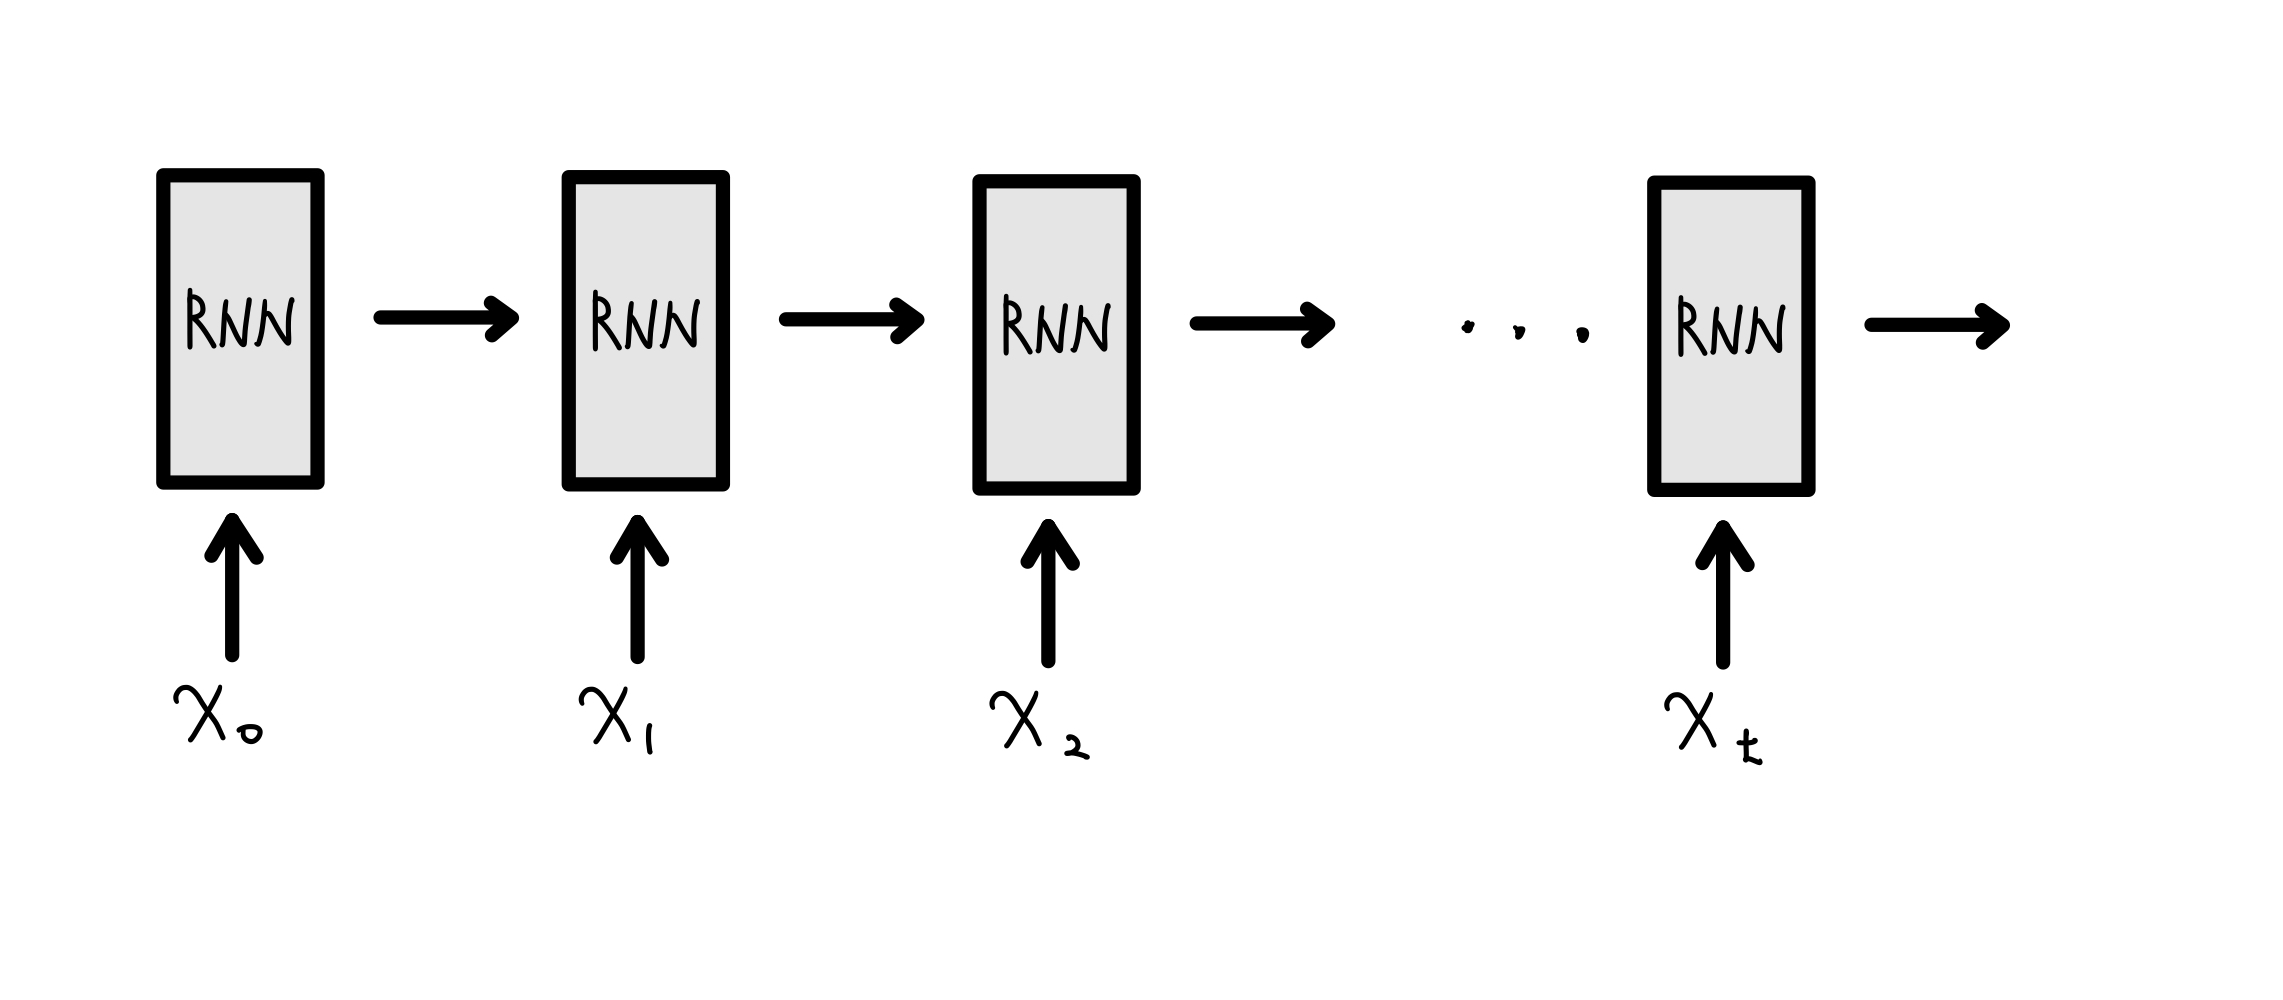
\includegraphics[width=\textwidth]{Figures/rnn.jpeg}
        \caption{RNN Model}
        \label{fig:rnn}
    \end{subfigure}
    \hfill
    \begin{subfigure}[b]{0.45\textwidth}
        \centering
        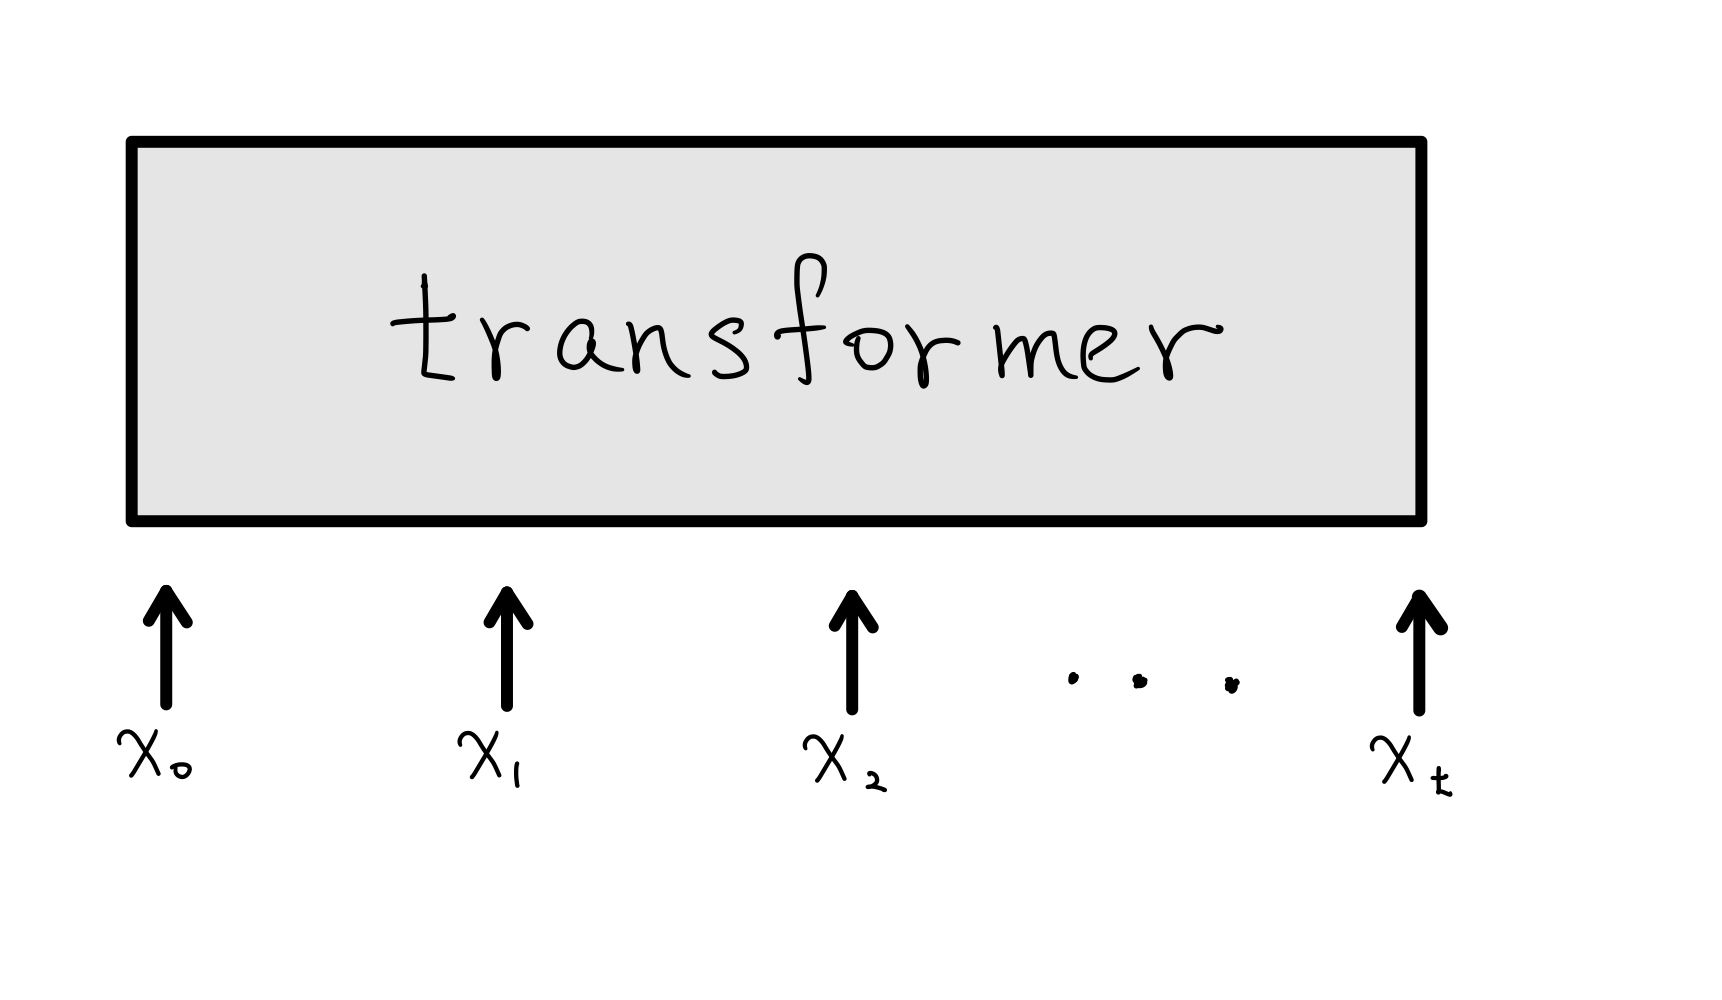
\includegraphics[width=\textwidth]{Figures/transformer.jpeg}
        \caption{Transformer Model}
        \label{fig:transformer}
    \end{subfigure}
    \caption{Comparison of RNN and Transformer architectures.}
    \label{fig:comparison}
\end{figure}

\subsection{Self-Attention Mechanism}

Self-attention is the core mechanism that allows Transformers to process and understand relationships within a sequence efficiently. Unlike traditional models that rely on sequential computations, self-attention allows each token in an input sequence to consider every other token simultaneously. This mechanism is particularly well-suited for high-energy physics applications, where complex dependencies exist between detector hits, and the order in which data is collected does not necessarily dictate meaningful relationships.

At its essence, the \textbf{attention mechanism} determines how much focus each token should place on other tokens when computing its representation. This is achieved by transforming each input into three vectors: a \textbf{query} (\( Q \)), a \textbf{key} (\( K \)), and a \textbf{value} (\( V \)). The query represents what a token is looking for in other tokens, the key encodes what information each token contains, and the value carries the actual content that gets passed forward. The attention scores are computed by measuring the similarity between queries and keys, which determines how much influence one token should have on another.

The scaled dot-product attention mechanism follows the equation:

\begin{equation}
\text{Attention}(Q, K, V) = \text{softmax} \left( \frac{QK^T}{\sqrt{d_k}} \right) V
\end{equation}

where \( d_k \) is the dimension of the key vectors, used as a scaling factor to stabilize gradients.

For detector simulations, this mechanism provides a significant advantage. Unlike models that process data sequentially, Transformers can immediately establish long-range dependencies, capturing interactions between hits that may be spatially distant but physically correlated. This ability to dynamically adjust attention across the dataset ensures that important features are preserved, leading to more accurate and efficient simulations.

Figure \ref{fig:self_attention} provides a visualization of this process, illustrating how input tokens are transformed and passed through attention layers. While the details of the computation involve matrix multiplications and scaling factors, the key idea remains straightforward: \textbf{each token learns to selectively focus on the most relevant information, allowing the model to capture both local and global dependencies simultaneously}. This capability is what makes Transformers particularly powerful, not only in natural language processing but also in scientific applications where capturing intricate relationships is essential.


\subsection{Types and Structure of Transformer Architectures}
The original Transformer architecture, as introduced by Vaswani et al., consists of both an encoder and a decoder. The encoder processes the input sequence, while the decoder generates the output sequence. This setup is particularly effective for tasks like machine translation. However, in practice, different applications benefit from using only the encoder or decoder.

\begin{figure}[ht]
    \centering
    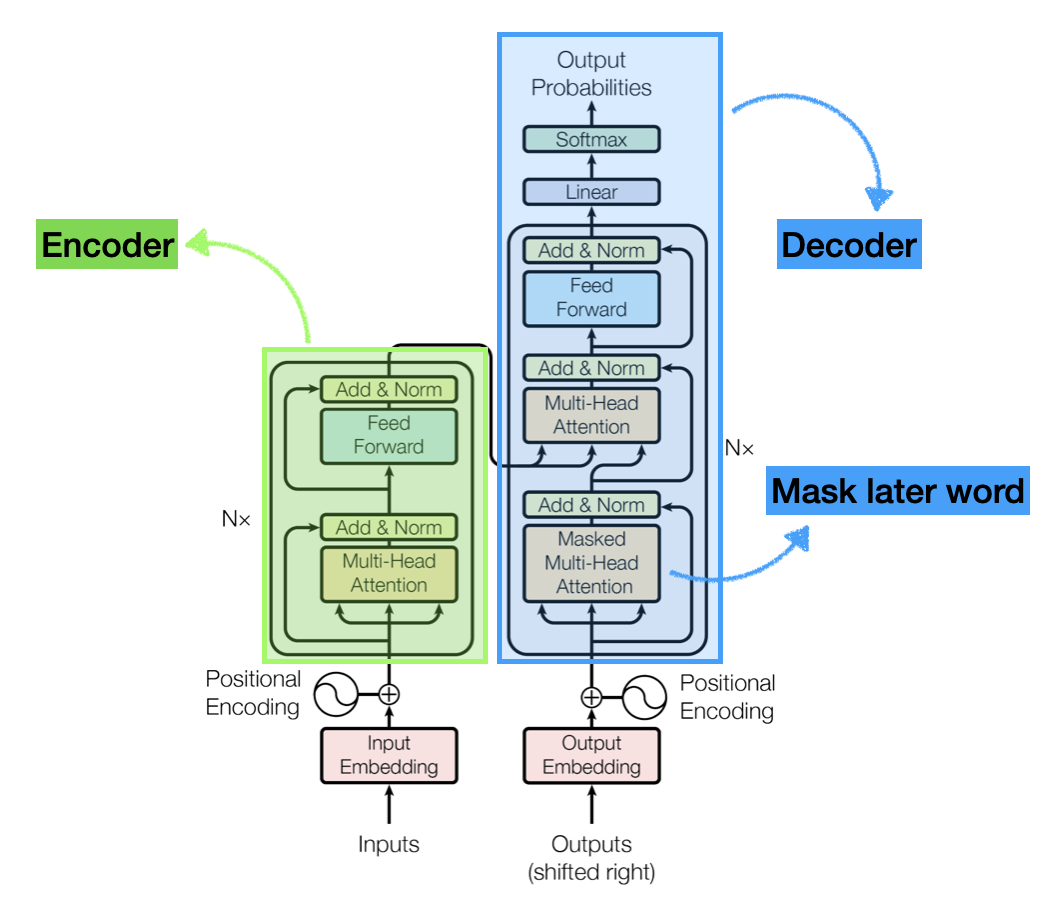
\includegraphics[width=0.8\textwidth]{Figures/transformerblock.png}
    \caption{The structure of the original Transformer model. Adapted from \textit{"Attention is All You Need,"} with additional annotations.}
    \label{fig:transformer_structure}
\end{figure}

The three main types of Transformer architectures are as follows:

\begin{itemize}
    \item \textbf{Encoder-only Models}: Encoder-only models, such as BERT, create contextual embeddings by attending to all tokens bidirectionally. These models are ideal for tasks requiring sequence understanding, like classification.
    
    \item \textbf{Decoder-only Models}: Decoder-only models, like GPT, are designed for unidirectional generation. Each token attends only to previous tokens, making these models suitable for tasks like language modeling.
    
    \item \textbf{Encoder-Decoder Models}: The original Transformer model combines both an encoder and a decoder, making it effective for sequence-to-sequence tasks such as machine translation. Examples include BART and T5.
\end{itemize}

\subsection{Choosing an Encoder-Only Model for Detector Simulation}
In the context of detector simulation, our objective is to generate a high-quality representation of input data, such as particle collisions. Given that our datasets exhibit rotational symmetry, an encoder-only model is the optimal choice, as it efficiently extracts and encodes essential features without introducing the additional complexity of a generative decoder. By focusing solely on representation learning, the encoder architecture ensures that the model captures the intricate relationships within the data while maintaining computational efficiency.


% \begin{figure}[ht]
%     \centering
%     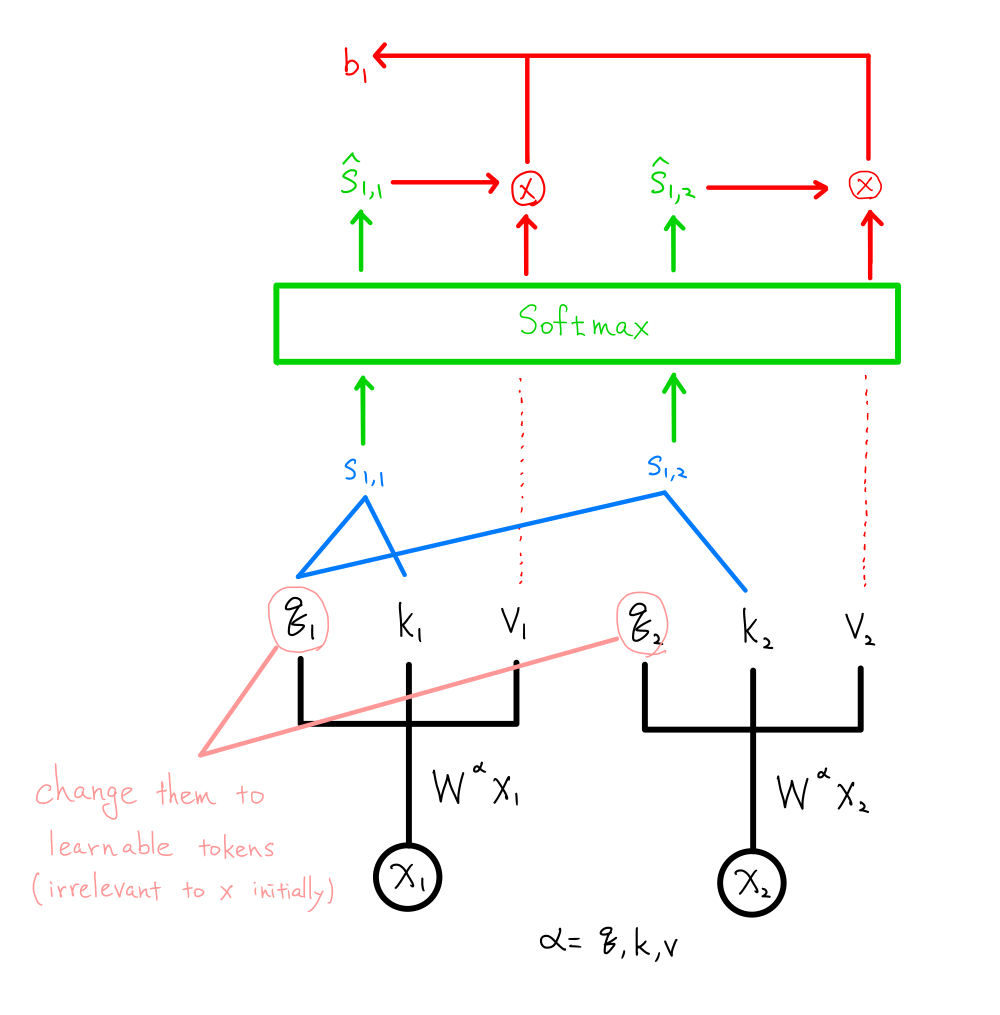
\includegraphics[width=0.8\textwidth]{Figures/attention.jpeg}
%     \caption{The concept of Self-attention mechanism in Transformers.}
%     \label{fig:self_attention}
% \end{figure}

\section{Our Model Structure}
Our model architecture builds upon the Transformer framework, with specific modifications to optimize performance in detector simulations, as shown in Figure \ref{fig:model_structure}.

\begin{figure}[ht]
    \centering
    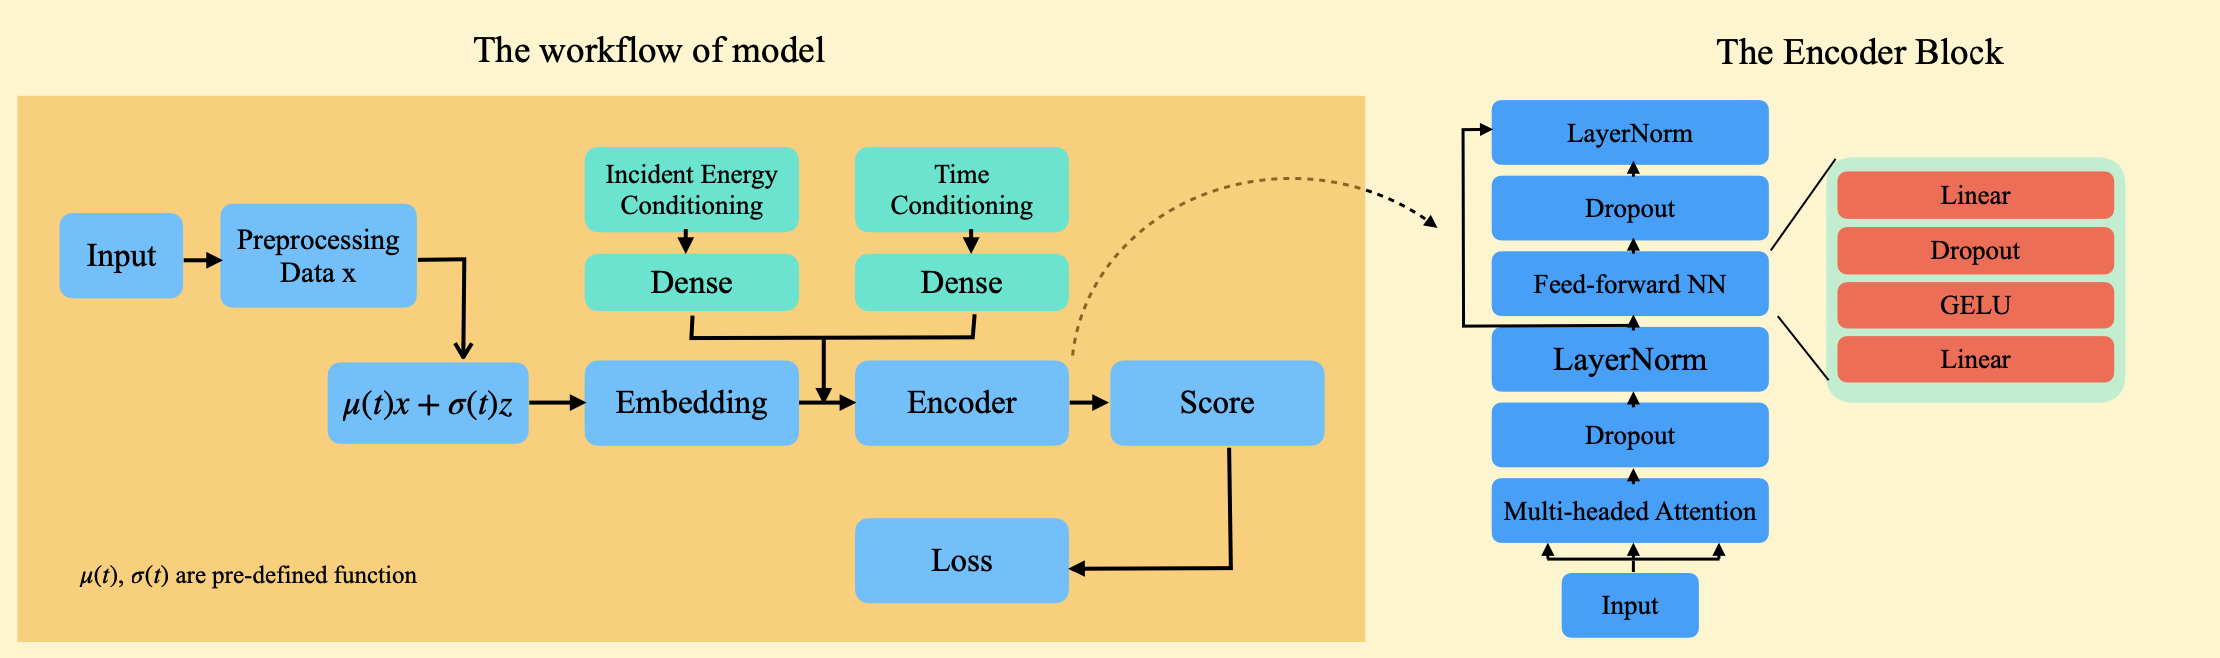
\includegraphics[width=0.8\textwidth]{Figures/model_structure1.png}
    \caption{Custom Transformer model structure for detector simulations.}
    \label{fig:model_structure}

\end{figure}
We incorporate \textbf{Gaussian Fourier Projections} \cite{tancik_fourier_2020} to effectively encode temporal information, dense layers to transform conditional variables, and \textbf{mean-field attention} \cite{kach_pay_2024} to efficiently aggregate global context. These architectural choices enable our model to capture complex dependencies, thereby enhancing the fidelity and accuracy of simulation outcomes.

\subsection{Gaussian Fourier Projection for Temporal Encoding}
The Gaussian Fourier Projection component encodes temporal information using Gaussian random features. This technique allows the model to incorporate high-frequency time-dependent information, in our case time and incident energy, which is crucial for capturing the dynamics of particle interactions within detectors.

In our model, we apply a Fourier feature mapping \( \gamma \) to featurize input coordinates before passing them through a coordinate-based multilayer perceptron (MLP). This approach improves both convergence speed and generalization.

The mapping function \( \gamma \) transforms input points \( \mathbf{v} \in [0, 1)^d \) onto the surface of a higher-dimensional hypersphere using sinusoidal functions:

\begin{equation}
\gamma(\mathbf{v}) = 
\begin{bmatrix}
a_1 \cos(2 \pi \mathbf{b}_1^T \mathbf{v}) \\ 
a_1 \sin(2 \pi \mathbf{b}_1^T \mathbf{v}) \\ 
\vdots \\ 
a_m \cos(2 \pi \mathbf{b}_m^T \mathbf{v}) \\ 
a_m \sin(2 \pi \mathbf{b}_m^T \mathbf{v})
\end{bmatrix}
\end{equation}

where \( a_i \) and \( \mathbf{b}_i \) are parameters that control the scaling and frequency of each sinusoid. We set \( a = 1 \) for all cases and experiment with different values of \( \mathbf{b} \) to identify optimal performance. The results are presented in subsequent sections.

\subsection{Mean-Field Attention in Detector Simulation}
Our model utilizes a variation of self-attention called \textbf{mean-field attention}. Unlike traditional self-attention, mean-field attention employs a class token to aggregate information from all tokens, creating a global summary. This reduces computational complexity while preserving essential global context.

Mean-field attention allows the class token to encapsulate the sequence's essential features by attending to each token once. This mechanism is computationally efficient and well-suited for high-energy physics applications, where capturing global properties of particle collisions is more important than individual token interactions. Figure \ref{fig:attention_comparison} provides a comparison between self-attention and mean-field attention mechanisms.

\begin{figure}[ht]
    \centering
    \begin{subfigure}[b]{0.35\textwidth}
        \centering
        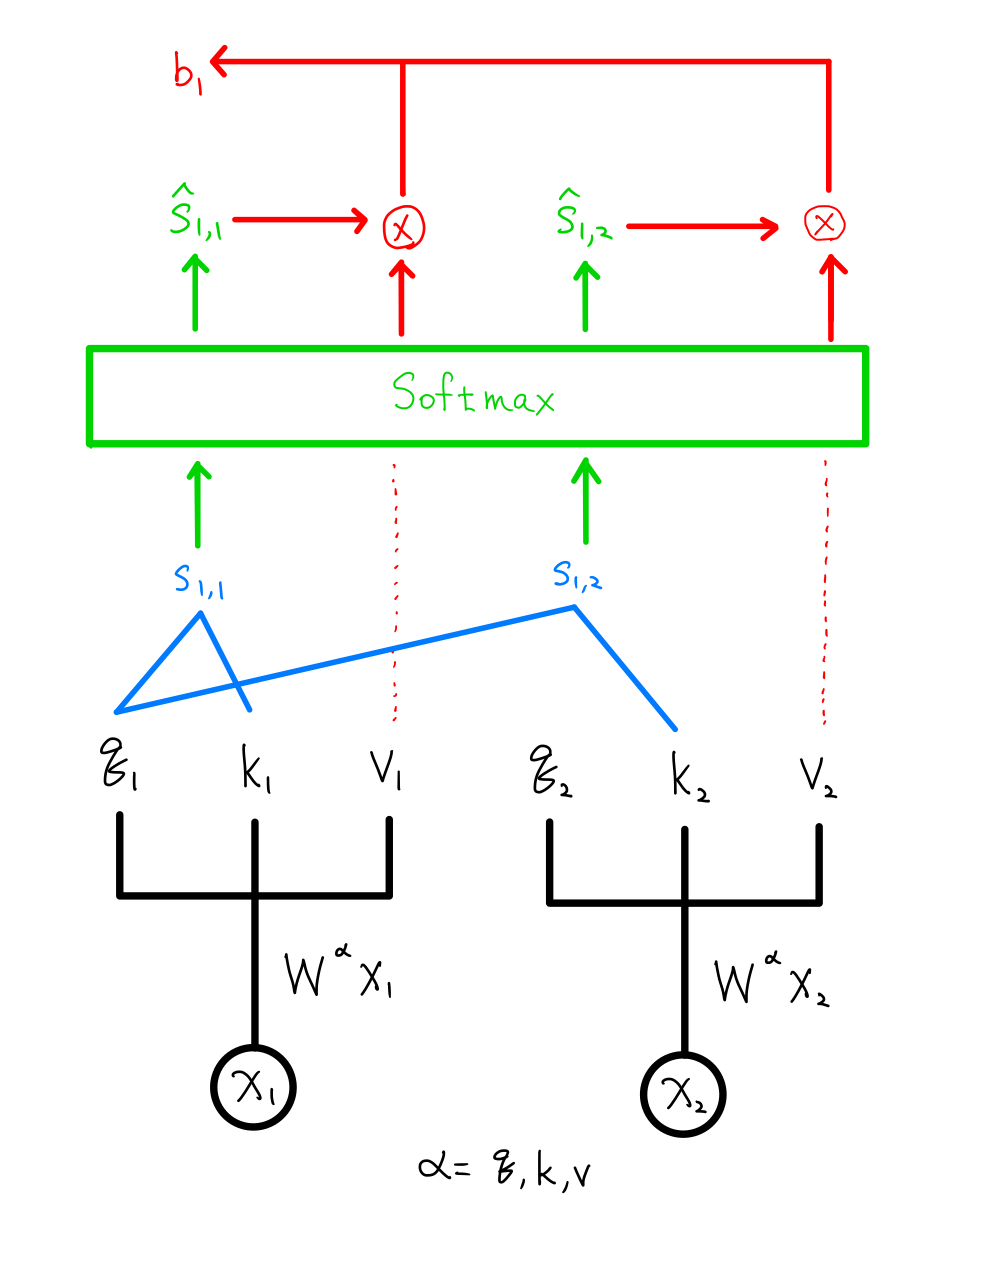
\includegraphics[width=\textwidth]{Figures/selfattention.jpeg}
        \caption{Self-Attention Mechanism}
        \label{fig:self_attention}
    \end{subfigure}
    \hfill
    \begin{subfigure}[b]{0.45\textwidth}
        \centering
        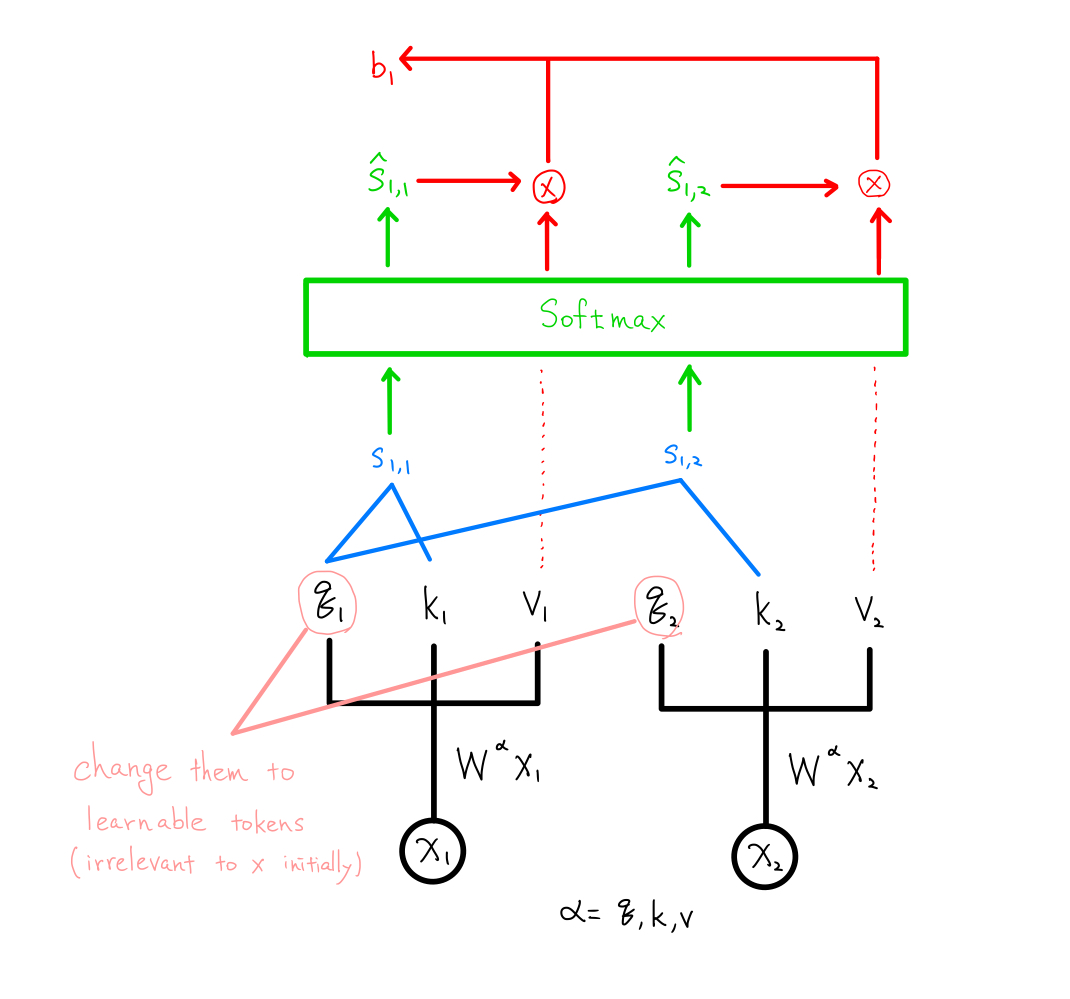
\includegraphics[width=\textwidth]{Figures/meanfield.jpeg}
        \caption{Mean-Field Attention Mechanism}
        \label{fig:mean_field_attention}
    \end{subfigure}
    \caption{Comparison of self-attention and mean-field attention mechanisms.}
    \label{fig:attention_comparison}
\end{figure}

% \subsection{Parameter Tuning}
% Once the model structure is established, tuning the parameters is essential for optimal performance. 

% To optimize the model, we utilize \textbf{Weights \& Biases (wandb)} for parameter tuning. Using wandb’s sweep functionality, we systematically explore hyperparameters, including:

% \begin{itemize}
%     \item \textbf{Number of blocks}: Controls the depth of the Transformer model.
%     \item \textbf{Number of heads}: Determines the number of attention heads in the multi-head attention mechanism.
%     \item \textbf{Hidden dimension}: Sets the size of the hidden layers in the model.
%     \item \textbf{Embed dimension}: Specifies the embedding size for the model’s input.
%     \item \textbf{Batch size}: Number of samples per batch.
%     \item \textbf{Learning rate}: Determines the rate at which the model updates during training.
%     \item \textbf{Dropout rate}: The fraction of nodes dropped during training to prevent overfitting.
%     \item \textbf{Sampling steps}: The number of sampling steps when solving SDE.
%     \item \textbf{Correction steps}: The number of correction steps in each sampling step.
%     \item \textbf{Scale in Fourier features}: The scaling factor for Fourier features.
% \end{itemize}

% The results of this tuning process are presented in later chapters.

\section{Conclusion}
Our custom Transformer model leverages specialized architectural choices to optimize performance in high-energy physics simulations. Key modifications include \textbf{Gaussian Fourier projections} for encoding time and incident energy, and \textbf{mean-field attention} for capturing global context beyond immediate shower information. The addition of a class token enables the model to represent both local and global dependencies, making it particularly suitable for scenarios with strong temporal and energetic relationships.

The mean-field attention mechanism enhances computational efficiency by reducing complexity while preserving essential global information. Parameter tuning plays a crucial role in achieving optimal performance, as we demonstrate with our use of wandb. By employing an encoder-only model, we capture inter-token relationships within the data, making our approach well-suited for high-energy physics applications.


% % Chapter 6. Results
\chapter{Strategies and Results}
\section{Data Preprocessing}

\subsection{Bucketing}
Before we explain why we need bucketing, we can first explain the structure of our data. When one particle interacts with the detector, it will produce a series of hits, which we call one shower. So in one shower, we have several hits, while one hit means one point in the detector labeled by the energy. One hit has several features, such as the hit energy, x, y and z coordinates. What's more, we will send several showers make it to be one batches to our model. So the structure of our data is actually a 3D tensor, where the first dimension is the number of showers, the second dimension is the number of hits in one shower, and the third dimension is the number of features in one hit.

In chapter 5, we have discussed that our model is a transformer-based model. While transformer implement the self-attention mechanism, it requires the length of the sequence to be fixed in each batches. However, the number of hits in each event varies, which makes it difficult to feed the data into the transformer. To address this issue, we would need to pad the sequences to a fixed length. What's more, the length of the data can vary from 1 to 5500, which means that the padding will be very large. This will lead to a waste of memory and computation. To solve this problem, we employed a bucketing strategy to group events with similar numbers of hits into the same bucket. This allowed us to pad the sequences within each bucket to a fixed length, making it easier to feed the data into the transformer. Based on the principle of similar memory usage, we divided the data into 45 buckets, each containing events with a similar number of hits. This bucketing strategy significantly improved the efficiency of the model and reduced the computational burden. Another advantage of bucketing is that we can first train the model on a smaller bucket to see if the model can learn the data well. If the model can learn the data well, we can then train the model on a larger bucket. This allows us to gradually increase the complexity of the data and ensure that the model can handle the data effectively.
\subsection{Preprocessor}

Preprocessing is a crucial step in preparing data for machine learning. Raw data often contains missing values, outliers, and features on different scales, which can negatively impact model performance. Effective preprocessing cleans and standardizes the data, ensuring consistency and enabling accurate predictions. It also helps models learn specific relationships between features more effectively.

A key role of preprocessing is improving data quality. Techniques like imputation, normalization, and outlier removal address missing or noisy values, allowing models to focus on meaningful patterns rather than irrelevant or erroneous information. Preprocessing also standardizes feature scales, ensuring equal contributions to models, which is especially critical for distance-based algorithms like neural networks or support vector machines.

Additionally, preprocessing optimizes computational efficiency by simplifying data complexity through methods like dimensionality reduction or sampling. This is vital for large-scale datasets, enabling faster and more resource-efficient training while preserving essential information. Overall, preprocessing is foundational for reliable, robust machine learning systems.

One important point to note is that we chose to use the x,y coordinate system instead of the cylindrical coordinate system. The primary reason for this choice is the discontinuity at $\theta=0$ and $\theta=2\pi$, which is unphysical and can introduce challenges during training. Although the cylindrical coordinate system aligns better with the detector structure and may simplify learning the relationship between radius and energy, we opted for the x,y coordinate system to ensure continuity and avoid such complications. 

From the reasons above, studying which preprocessing method is the best for our data is necessary. Below are some preprocessing methods we have tried and their results.

\begin{itemize}
    \item \textbf{RobustScalar}
    \begin{figure}[ht]
        \centering
        % Include your figure here
        \caption{RobustScalar}
    \end{figure}
    \item \textbf{QuantileTransformer}
    \begin{figure}[ht]
        \centering
        % Include your figure here
        \caption{RobustScalar}
    \end{figure}
    \item \textbf{StandardScaler}
    \begin{figure}[ht]
        \centering
        % Include your figure here
        \caption{RobustScalar}
    \end{figure}
    \item \textbf{MinMaxScaler}
    \begin{figure}[ht]
        \centering
        % Include your figure here
        \caption{RobustScalar}
    \end{figure}
    \item \textbf{Specail Transformation from other papers}
    \begin{figure}[ht]
        \centering
        % Include your figure here
        \caption{RobustScalar}
    \end{figure}
\end{itemize}


The reason of choosing x y coordinate rather than spherical coordinate
\section{Metrics}
\subsection{FID Score}
To evaluate the performance of our model, we employed the Fréchet Inception Distance (FID) score as a key metric. The FID score is widely used to assess the quality of generated samples by measuring the distance between the feature representations of real and generated images using the InceptionV3 model \cite{inceptionv3}. A lower FID score indicates that the generated samples are closer to the real samples in terms of their statistical distribution. We utilized the PyTorch library's implementation of the FID score \cite{pytorch} for our calculations. The FID score is calculated as follows:

For two multivariate Gaussian distributions with means $\mu_{\text{real}}$ and $\mu_{\text{gen}}$ and covariance matrices $\Sigma_{\text{real}}$ and $\Sigma_{\text{gen}}$, the FID score is given by:

\begin{equation}
    \text{FID} = ||\mu_{\text{real}} - \mu_{\text{gen}}||^2 + \text{Tr}(\Sigma_{\text{real}} + \Sigma_{\text{gen}} - 2(\Sigma_{\text{real}}\Sigma_{\text{gen}})^{1/2}),
\end{equation}

In order to measure what's the performance on each dimension, we also calculate the FID score on each dimension. Then the FID score on each dimension is calculated as follows:

\begin{equation}
    \text{FID}_{\text{dim}} = ||\mu_{\text{real}} - \mu_{\text{gen}}||^2 + \text{Tr}(\sigma_{\text{real}} + \sigma_{\text{gen}} - 2(\sigma_{\text{real}}\sigma_{\text{gen}})^{1/2}),
\end{equation}

One important point to note is that sometimes the FID score is not enough to evaluate the performance of the model. For example, if the FID score is low, it means that the generated samples are close to the real samples in terms of their statistical distribution. However, the generated samples may not capture the underlying physics of the data, for example, the shape of the data may not be the gaussian distribution. In this case, the FID score may not be a good metric to evaluate the performance of the model. So when we evaluate the performance of the model, we still need to rely on other metrics and observation.

\subsection{Classifier}

As mentioned earlier, the FID score alone is insufficient for evaluating the performance of the model. To complement it, we employ classifiers to assess the model's ability to generate realistic samples. These classifiers are binary, designed to distinguish between real and generated samples. The structure of the classifiers is primarily based on deep neural networks (DNNs). The input features for the classifiers can range from high-level features, such as energy distributions across layers or $\theta$ bins, to low-level features like the energy values in each voxel. Regardless of the input, real samples are labeled as 1, and generated samples are labeled as 0. The loss function used is the Binary Cross-Entropy Loss (\texttt{BCEWithLogitsLoss}).

However, our classifiers consistently achieve very high performance, with an AUC of 99--100\%. This indicates that it is relatively easy for the classifier to distinguish between real and generated samples. This issue is not unique to our study; many papers report similar findings, even when their models achieve low FID scores and realistic data shapes. One plausible explanation is that generated samples tend to exhibit higher continuity, while real data has inherent discreteness due to the limitations of the detector. This mismatch in continuity could make it easier for classifiers to identify generated samples.

% Add this section's details as necessary.

\section{VE and VP Studies}
As mentioned before, there are two main ways to add the noise into the data, which are Variance Exploding (VE) and Variance Preserving (VP). In this section, we will discuss the performance of the model trained with these two methods. First, we can observe the standard deviation of the data after adding the noise. We can see that the change of the standard deviation is more steep at the begining in VE method than VP method. This means that the VE method has more power to push the data to the random noise, which is the initial state of the sampling space. That is why we guess the VE method will have a better performance than the VP method.

\begin{figure}[h!]
    \centering
    % Include your loss shape figure here
    \caption{Mean std*noise for energy distribution.}
\end{figure}

Next, we can further compare the actual distribution change after adding the noise. We can see that the distribution of the data after adding the noise in the VE method is more close to the random noise than the VP method. This is consistent with our guess that the VE method will have a better performance than the VP method.

\begin{figure}[h!]
    \centering
    % Include your loss shape figure here
    \caption{The distribution of the data after adding the noise.}
\end{figure}

We also compared the FID scores of models trained with the VE and VP methods. The results showed that the VE method resulted in a lower FID score compared to the VP method. This suggests that the VE method is more effective at pushing the model toward generating random samples that better represent the initial sampling space.

\begin{figure}[h!]
    \centering
    % Include your FID score comparison figure here
    \caption{Comparison of FID scores for VE and VP methods.}
\end{figure}

In conclusion, the VE method outperformed the VP method in terms of FID score. 
We guess this is because it has more power to push our data to random noise, which is the initial state of sampling space. So our model know how to do the reverse process at the beginning in VE method. For example, if we see the standard deviation of both VE and VP methods, one can find out VE has the steeper slope than VP, which means it has the power to push the data to the random noise.

\section{$\sigma_{max}$ and $\sigma_{min}$ Studies}

Among all fo the parameters, the $\sigma_{max}$ may be the most important one. In the context of diffusion models, the parameters $\sigma_{max}$ and $\sigma_{min}$ play a crucial role in determining the noise levels introduced during the forward and backward processes. These parameters define the range of noise scales, influencing both the quality of the generated samples and the training stability of the model. This section explores the impact of $\sigma_{max}$ and $\sigma_{min}$ on model performance and provides insights into selecting optimal values for these parameters.

\subsection{The Role of $\sigma_{max}$ and $\sigma_{min}$}

The parameter $\sigma_{min}$ represents the minimum noise level in the forward process and also used as the step size of $\sigma$ series. In this case as you can imagine, $\sigma_{min}$ is typically set close to zero. However, based on our abservation, $\sigma_{min}$ won't actually affect too mcuh on the performance of our model. Conversely, $\sigma_{max}$ deos. It defines the maximum noise level and is set high enough to approximate a standard normal distribution. And it also determines the power to change our data distribution during the training. These noise levels influence the progression of the diffusion process, as the model learns to reverse the added noise during training.

Larger $\sigma_{max}$ ensures sufficient diversity in the data during the forward process, helping the model generalize better. Yet, if $\sigma_{max}$ is too large, it can result in excessively noisy samples, making it challenging for the model to learn the reverse process effectively.

\begin{figure}[ht]
    \centering
    % Include your figure here
    \caption{The result of different $\sigma_{max}$ and $\sigma_{min}$ in both VE and VP.}
\end{figure}

\subsection{Conclusions}

As shown in the results, the choice of $\sigma_{max}$ and $\sigma_{min}$ significantly impacts the performance of the model. Larger $\sigma_{max}$ values can improve the diversity of the data and enhance the model's generalization ability. However, setting $\sigma_{max}$ too high can lead to noisy samples and hinder the model's learning process. On the other hand, $\sigma_{min}$ has a less pronounced effect on model performance, as it primarily serves as the step size for the noise levels. And based on our data scale, we choose $\sigma_{min}$ to be 0.0003, and $\sigma_{max}$ to be 5.0 in VE.

\section{Overall Parameter Sweeping}
Besides, the parameters mentioned above there are also a lot of other parameters that can affect the performance of the model or the memory allocation. Thus, we conducted a parameter sweeping study using \texttt{wandb}. We experimented with various learning rates, batch sizes, and hidden dimensions. Our findings indicated that the best-performing parameter configuration was:
\begin{itemize}
    \item Learning rate: $0.0003$
    \item Batch size: $128$
    \item Embedding dimension: $96$
    \item Hidden dimension: $96$
    \item Number of Attention Heads: $8$
    \item Number of Encoder Blocks : $16$
    \item Dropout rate: $0.2$
    \item Sampler Step: $100$
    \item Correction Step: $25$
    \item SDE : VE
    \item Sigma Max: $5.0$
    \item Sigma Min: $0.0003$
\end{itemize}

\begin{figure}[h!]
    \centering
    % Include your parameter sweeping study figure here
    \caption{Visualization of parameter sweeping results.}
\end{figure}


\section{Centralization}
After visualizing 2D or 3D plots revealed that the model failed to capture the relationship between energy and radius. A key observation was that the model could not learn that higher energy values should be concentrated near the center (smaller radii). Consequently, while the 1D plots were satisfactory, the generated samples lacked proper centralization.

To address this, we first tried to transform our data into spherical coordinate and introduce a correlation term between energy and theta in the loss function to try to suppress relation between energy and theta, hoping our model can thus learn more about the relation between energy and radius. 

The new loss function is defined as:
\begin{equation}
    L = L_{\text{MSE}} + \lambda L_{\text{cor}},
\end{equation}
where $L_{\text{MSE}}$ is the mean squared error loss, $L_{\text{cor}}$ is the correlation loss, and $\lambda$ is a weighting factor for the correlation loss. The correlation loss is defined as:
\begin{equation}
    L_{\text{cor}} = \frac{1}{N} \sum_{i=1}^{N} (x_i - \bar{x})(y_i - \bar{y}),
\end{equation}
where $x$ and $y$ are the variables of interest, and $\bar{x}$ and $\bar{y}$ are their respective means.

The reason why we don't apply the correlation term between energy and radius is that the relation between them is by experienced, although everyone would expect the result, it's not solid, we don't want to bias our model, or you can say we don't want to tell the answer of the relation to our model. 

However, although the correlation term was added to the loss function and it indeed suppressed the relation between energy and theta, the centralization of the generated samples did not improve significantly. This suggests that the correlation term alone is not sufficient to address the centralization issue.

\begin{figure}[h!]
    \centering
    % Include any relevant results or visualizations here
    \caption{The Picture after adding the correlation term.}
\end{figure}

After that, one time when we tried to use QuantileTransformer to preprocess the data, we found that the centralization of the data is improved. This is because the QuantileTransformer can transform the data to follow a uniform or a normal distribution. This can help the model to learn the data better, especailly the x,y distribution. This also makes it is able to learn the relation between energy and radius better.

The result compared to the original one is shown below:

\begin{figure}[h!]
    \centering
    % Include any relevant results or visualizations here
    \caption{The Comparison Picture after using QuantileTransformer.}
\end{figure}

\section{Conditioning Issue}
\subsection{incident energy}
With the optimal settings, our model was able to generate the basic shapes of both the energy and spatial distributions. However, the model often produced an excessive number of hits (\texttt{nhits}) at higher energy levels, leading to overestimation. This issue was not observed when training on single-bucket data, indicating that the model struggles to differentiate between data from different buckets. This suggests that our conditional variables are not functioning effectively. As you can see the result of energy deposit of single bucket data and all bucket data, the model can generate the data well in single bucket data, but it failed to generate the data well in all bucket data. This is because the model can't learn the condition well.

\begin{figure}[ht]
    \centering
    % Include your figure here
    \caption{The result of energy deposit of single bucket data and all bucket data.}
\end{figure}

To address this issue, we first need to make sure if our conditional variables aren't really working. So we tried to add the incident energy as the conditional variables and not. The result is shown below:

\begin{figure}[ht]
    \centering
    % Include your figure here
    \caption{The result of energy deposit with and without incident energy as conditional variables.}
\end{figure}

They are basically the same, indicating that the conditional variables are not working. Next, we also tried to concatenate the incident energy with the input data instead of adding them and the result is shown below:

\begin{figure}[ht]
    \centering
    % Include your figure here
    \caption{The result of energy deposit with incident energy concatenated with the input data.}
\end{figure}

As you can see, the result is totally a disaster. To be honest, we still don't know why this happened. 

Next, we move to even more complex conditional variables. We have tried class token, MoE. The result is shown below:

\begin{figure}[ht]
    \centering
    % Include your figure here
    \caption{The result of energy deposit with class token and MoE.}
\end{figure}

\subsection{time}

We also attempted to incorporate time as a conditional variable in our model. However, the results differ from those observed with incident energy. Even without explicitly using time as a condition, the output layer implicitly incorporates its effect by dividing by the standard deviation of the stochastic differential equation (SDE), which is time-dependent. Despite this, the inclusion of time as a conditional variable does not appear to enhance the model's performance.

The plot of loss versus time reveals consistent behavior across epochs, showing that the shape of this plot remains virtually unchanged. Notably, the loss value at $t = 0$ is almost identical to the initial loss, indicating that the time condition fails to improve the model's capacity to learn the data effectively.

Time close to $t = 0$ represents the critical phase where the model transitions toward generating real data, whereas near $t = 1$, the model predominantly learns the structure of Gaussian noise. This suggests that the model's learning mechanism may inherently prioritize earlier time steps, making additional time conditioning redundant or ineffective.

\begin{figure}[ht]
    \centering
    % Include your figure here
    \caption{The loss vs time plot.}
\end{figure}







% % Chapter 7. Conclusion and Discussion
\chapter{Future Goals}

Looking ahead, there are two primary objectives for future work:

\section{Further Acceleration of the Model}
The first goal is to further improve the speed of the model. Currently, our model achieves a 500x speedup compared to Geant4 simulations. However, there is potential for even greater acceleration by exploring alternative methods. For instance, replacing the Stochastic Differential Equation (SDE) framework with an Ordinary Differential Equation (ODE) approach, or implementing a restart method as suggested in \cite{restart}, could lead to significant improvements in computational efficiency.

\section{Layer Relationship Learning and Tracking}
The second goal is to enhance the model's ability to learn the relationships between layers. Specifically, we aim to train the model to identify which hits in one layer correspond to hits in the previous layer. This capability would enable the development of a model for particle tracking, providing a more comprehensive and detailed understanding of the underlying physical processes.

Achieving these goals would not only improve the current model but also open new possibilities for its application in simulation and analysis.



%----------------------------------------------------------------------------------------
%	THESIS CONTENT - APPENDICES
%----------------------------------------------------------------------------------------

\appendix % Cue to tell LaTeX that the following "chapters" are Appendices

% Include the appendices of the thesis as separate files from the Appendices folder

% A. Updates from the result presented in 2020 KAON
% % Appendix A

\chapter{Figures} % Main appendix title

\label{AppendixA} % For referencing this appendix elsewhere, use \ref{AppendixA}

% outline
%----------------------------------------------------------------------------
% 
%

\section{Best Result for Full Dataset}


\begin{figure}[htbp]
    \centering
    % First row: 4 figures
    \begin{subfigure}[b]{0.23\textwidth}
        \centering
        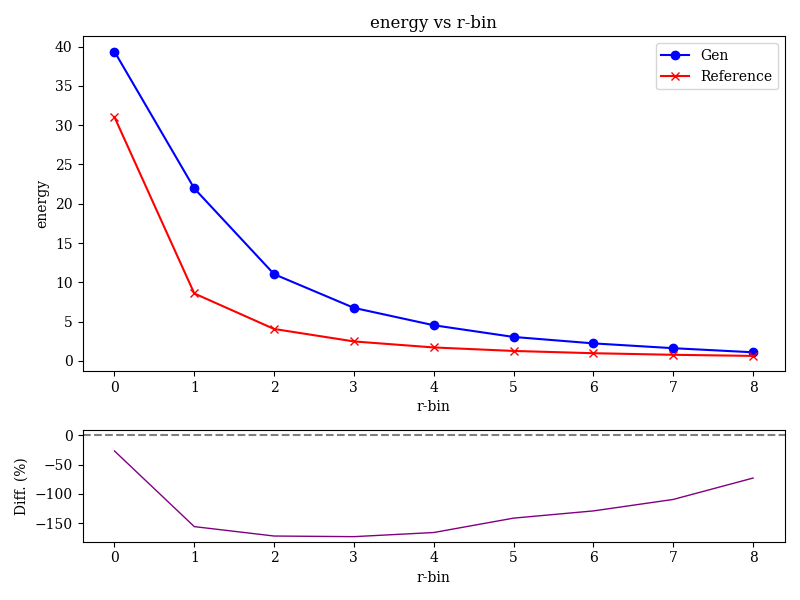
\includegraphics[width=\textwidth]{Figures/a1_2.png}
        \caption{Energy vs Radius}
        \label{fig:a1-2}
    \end{subfigure}
    \hfill
    \begin{subfigure}[b]{0.23\textwidth}
        \centering
        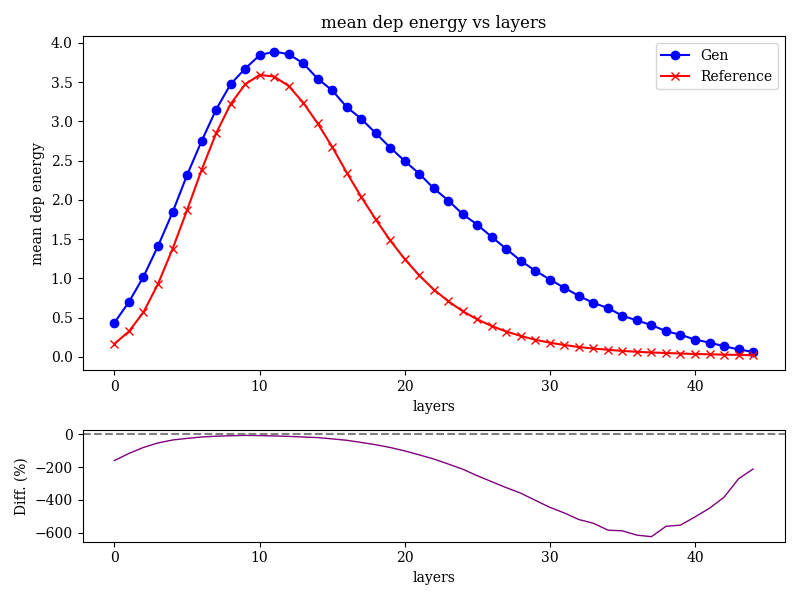
\includegraphics[width=\textwidth]{Figures/a1_3.png}
        \caption{Energy vs Z}
        \label{fig:a1-3}
    \end{subfigure}
    \hfill
    \begin{subfigure}[b]{0.23\textwidth}
        \centering
        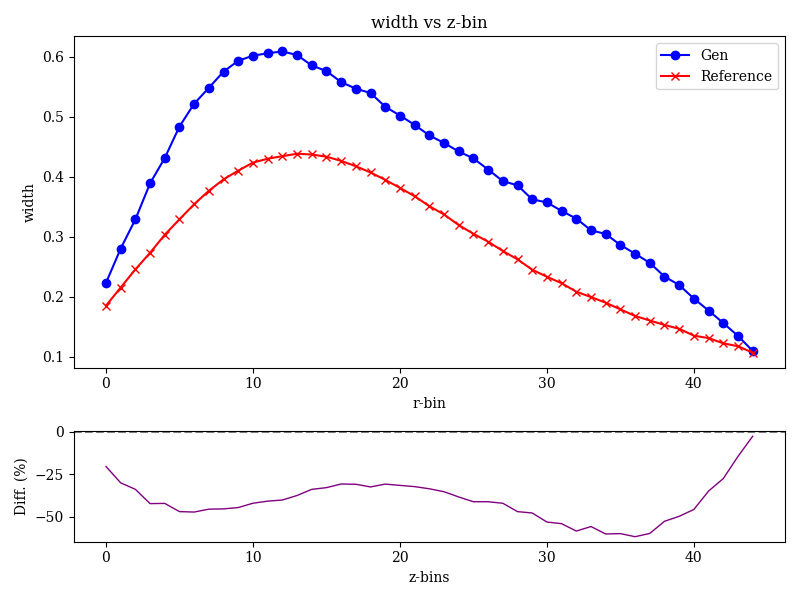
\includegraphics[width=\textwidth]{Figures/a1_4.png}
        \caption{R-width vs Layers}
        \label{fig:a1-4}
    \end{subfigure}
    \hfill
    \begin{subfigure}[b]{0.23\textwidth}  % Adjust width to fit 4 figures
        \centering
        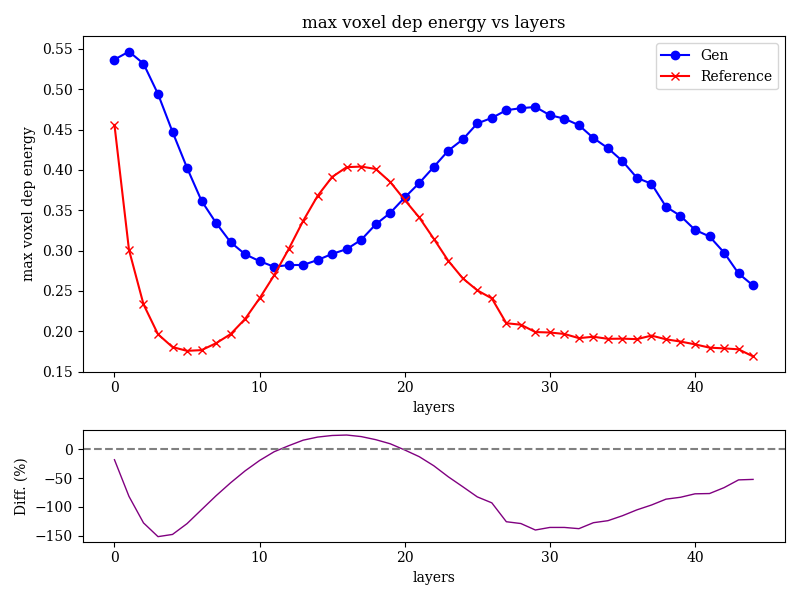
\includegraphics
        [width=\textwidth]{Figures/a1_5.png}
        \caption{Max Voxel Deposit vs Layers}
        
        \label{fig:a1-1}
    \end{subfigure}
    
    \vspace{0.6cm} % Space between rows

    % Second row: 3 figures
    \begin{subfigure}[b]{0.3\textwidth}  % Adjust width to fit 3 figures
        \centering
        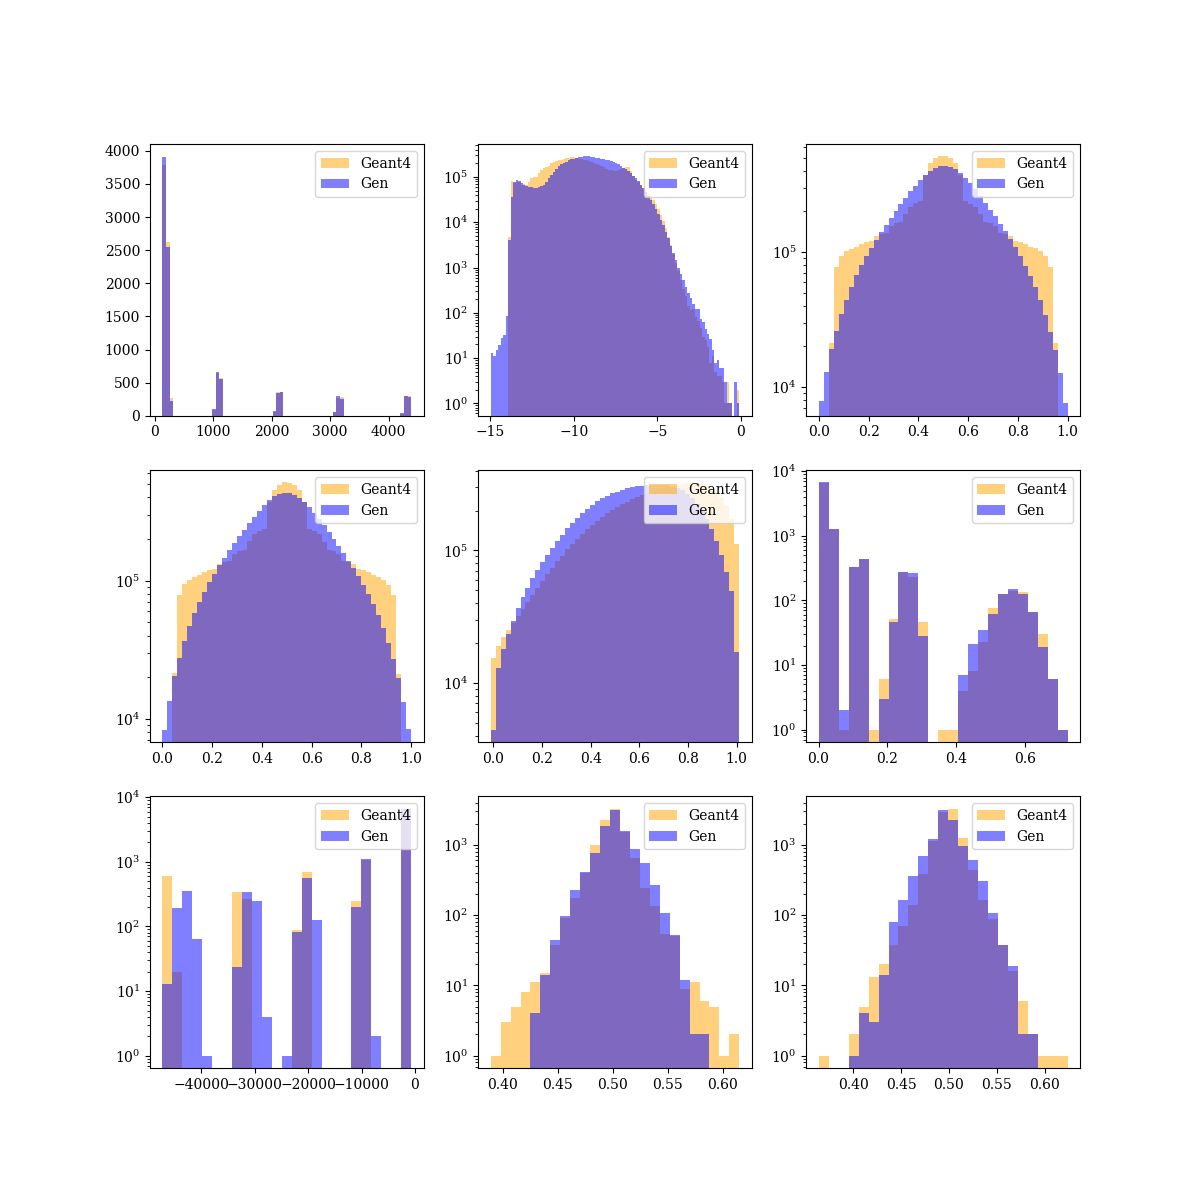
\includegraphics
        [width=\textwidth]{Figures/a1-1.png}
        \caption{1D Histogram}
        \label{fig:a1-5}
    \end{subfigure}
    \hfill
    \begin{subfigure}[b]{0.3\textwidth}
        \centering
        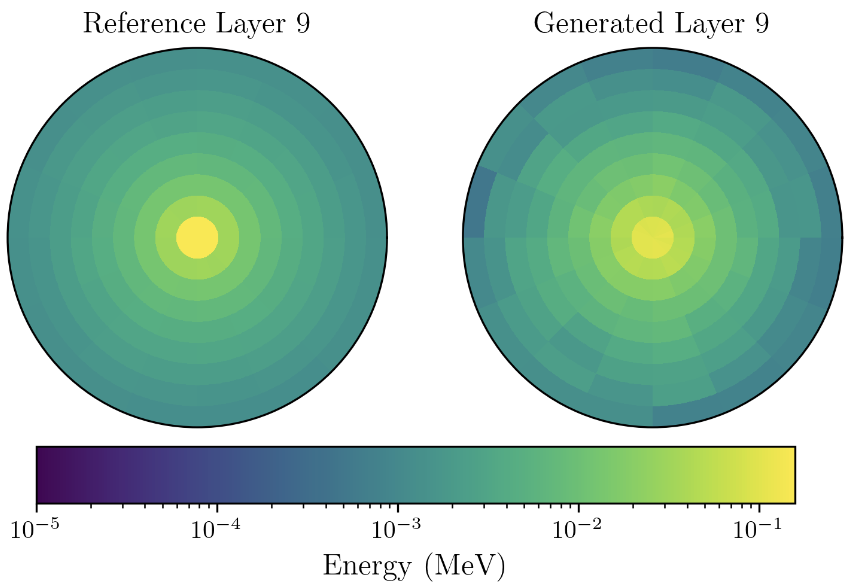
\includegraphics[width=\textwidth]{Figures/comparison.png}
        \caption{Energy voxel comparison}
        \label{fig:a1_5}
    \end{subfigure}
    \hfill
    \begin{subfigure}[b]{0.3\textwidth}
        \centering
        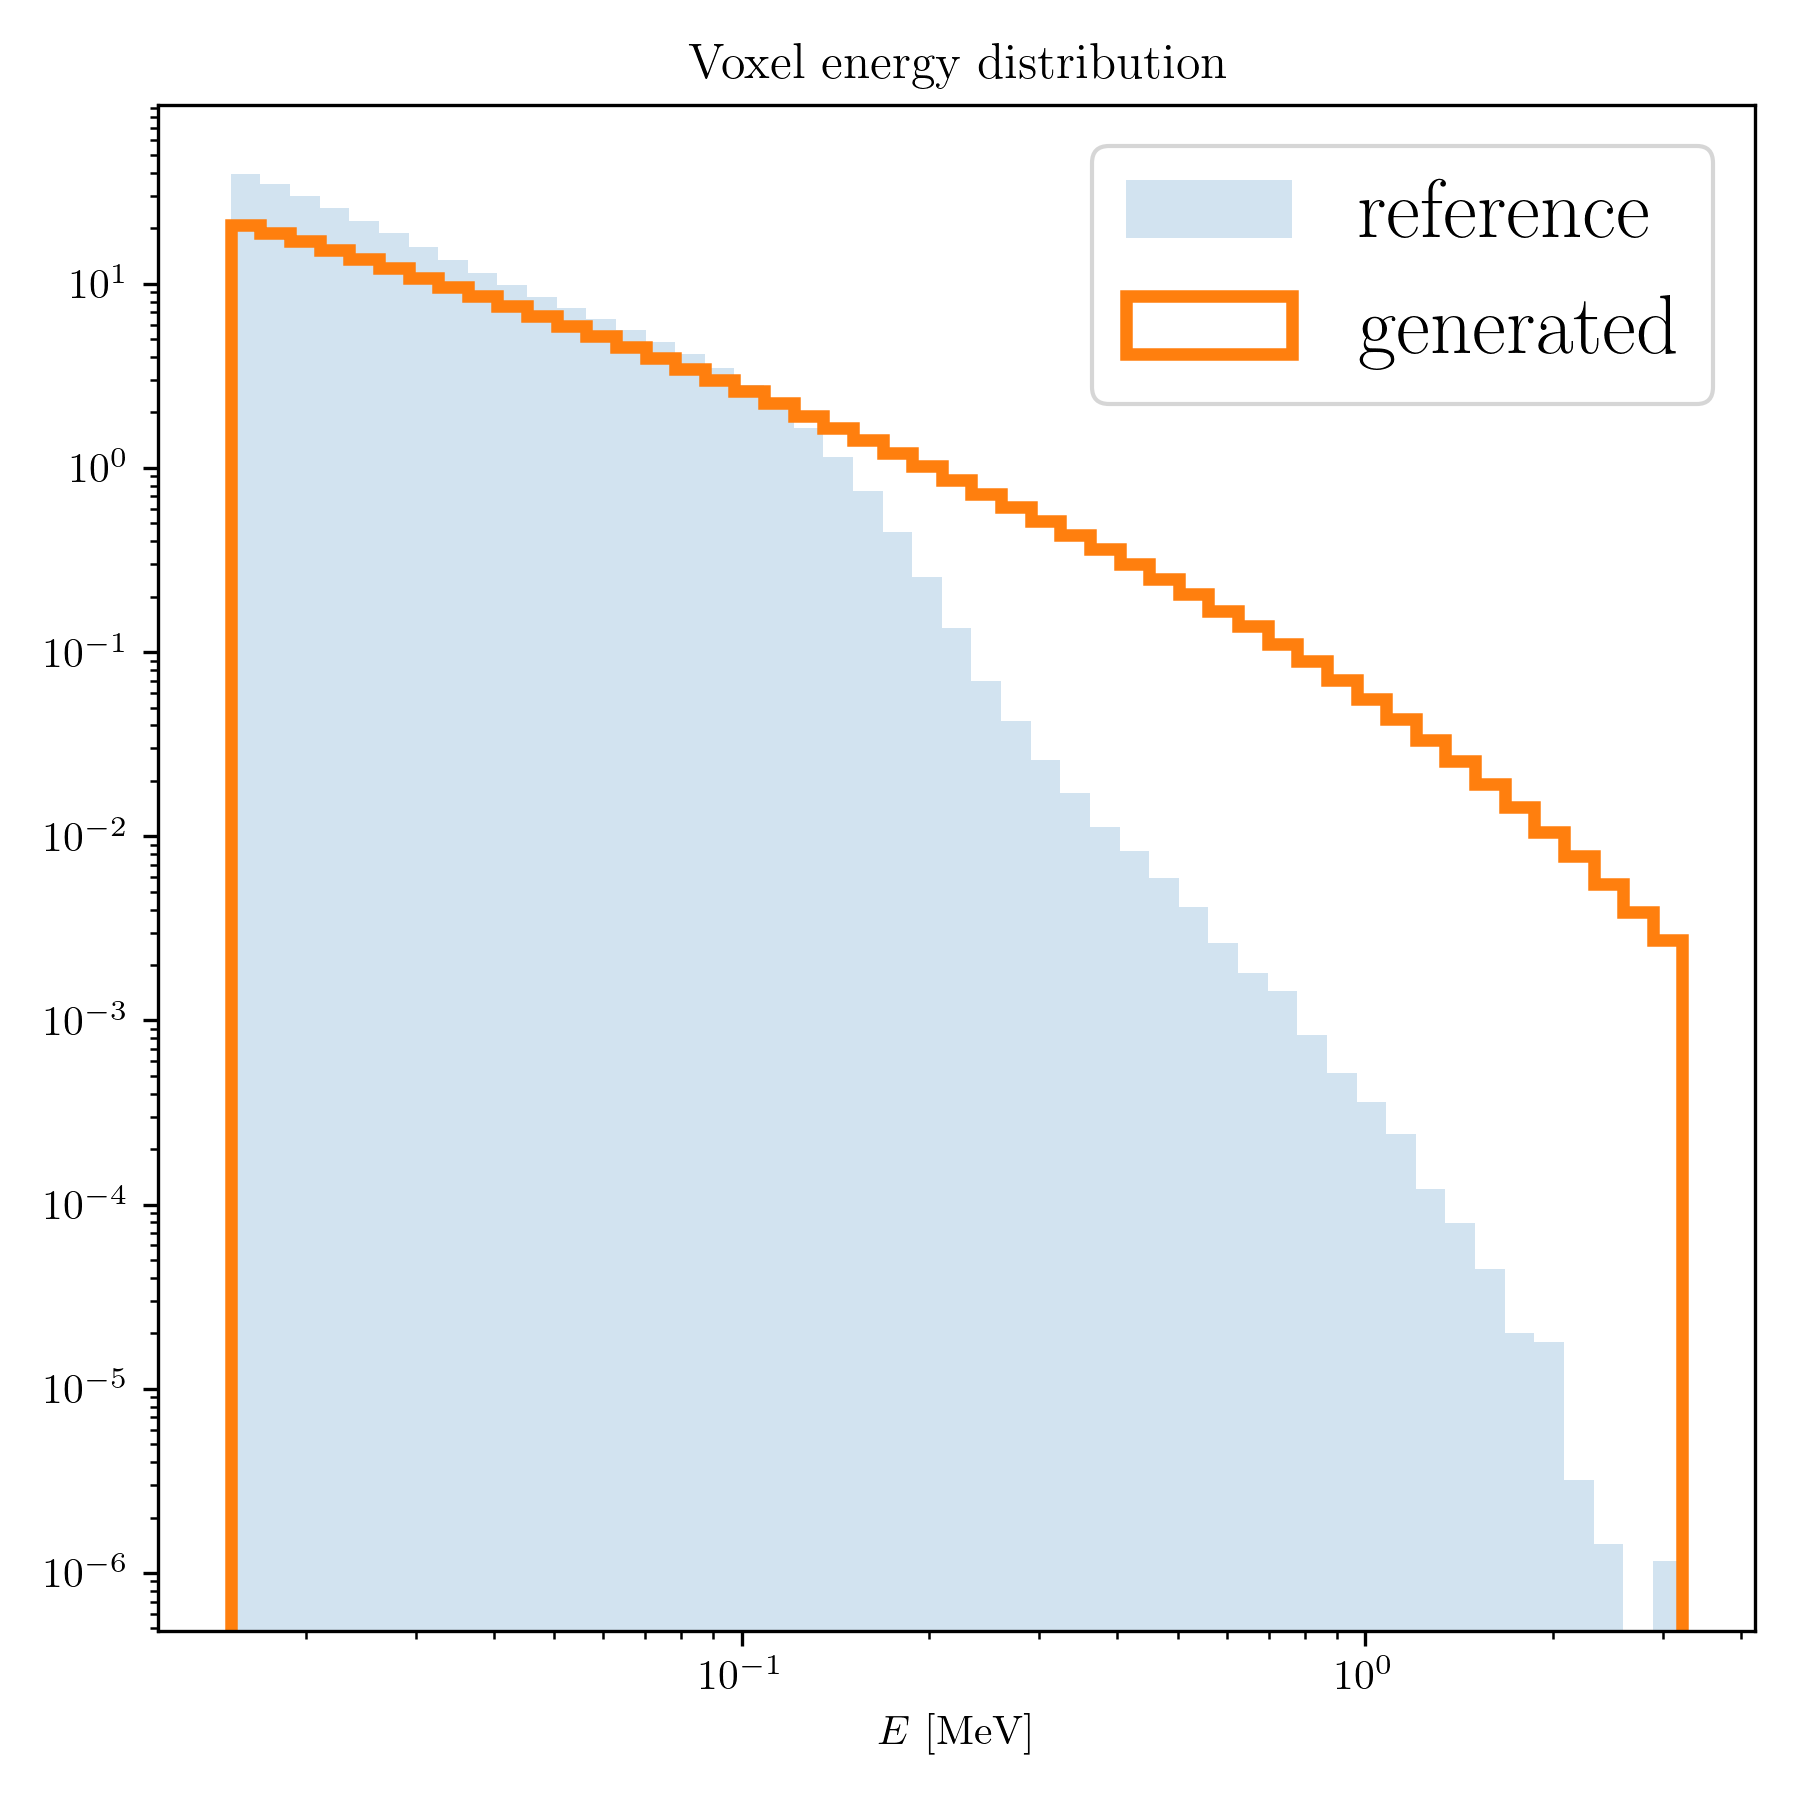
\includegraphics[width=\textwidth]{Figures/a1_7.png}
        \caption{Energy Deposit}
        \label{fig:a1_7}
    \end{subfigure}
\end{figure}

\newpage
\section{Best Result for Single Bucket Data}


\begin{figure}[htbp]
    \centering
    % First row: 4 figures
    \begin{subfigure}[b]{0.23\textwidth}
        \centering
        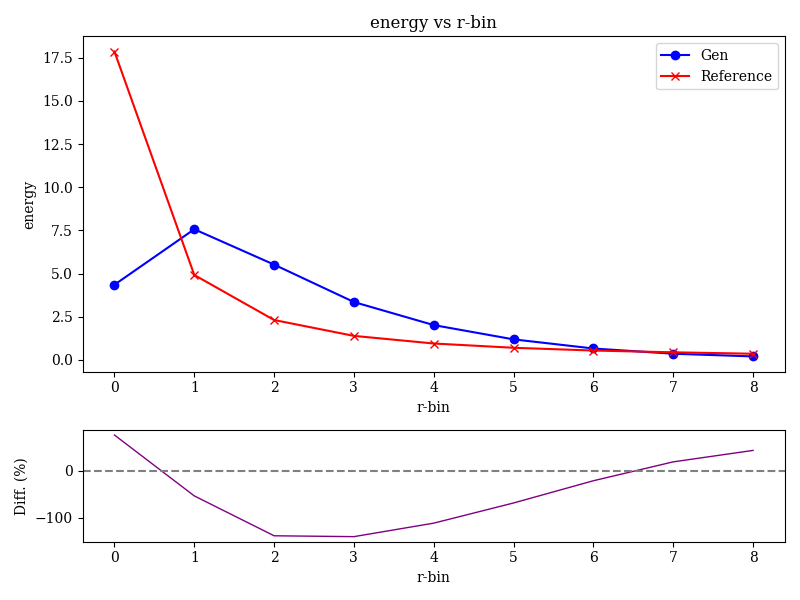
\includegraphics[width=\textwidth]{Figures/2_2.png}
        \caption{Energy vs Radius}
        \label{fig:a2_2}
    \end{subfigure}
    \hfill
    \begin{subfigure}[b]{0.23\textwidth}
        \centering
        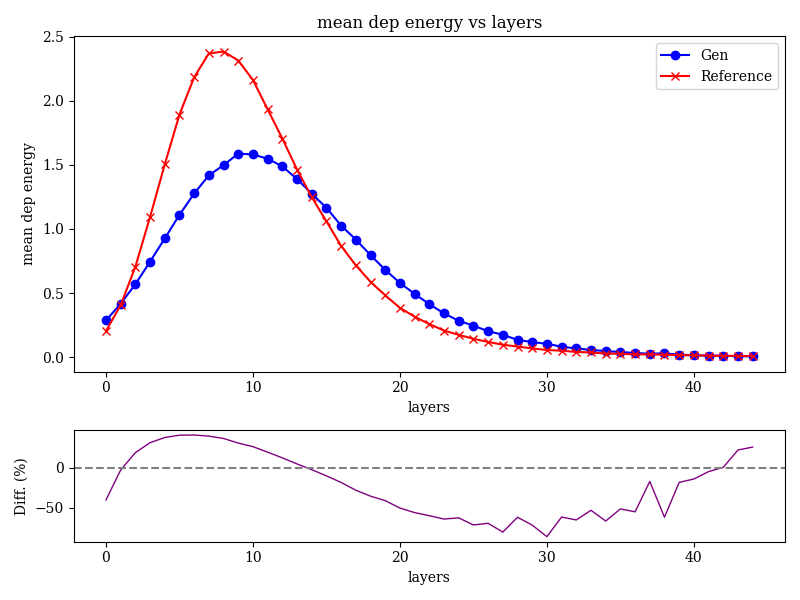
\includegraphics[width=\textwidth]{Figures/2_3.png}
        \caption{Energy vs Z}
        \label{fig:a2_3}
    \end{subfigure}
    \hfill
    \begin{subfigure}[b]{0.23\textwidth}
        \centering
        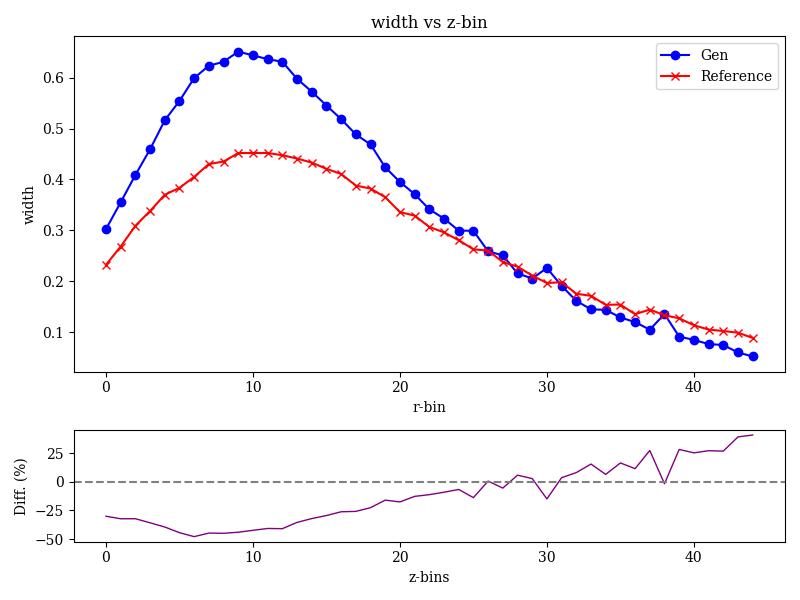
\includegraphics[width=\textwidth]{Figures/2_4.png}
        \caption{R-width vs layers}
        \label{fig:a2_4}
    \end{subfigure}
    \hfill
    \begin{subfigure}[b]{0.23\textwidth}  % Adjust width to fit 4 figures
        \centering
        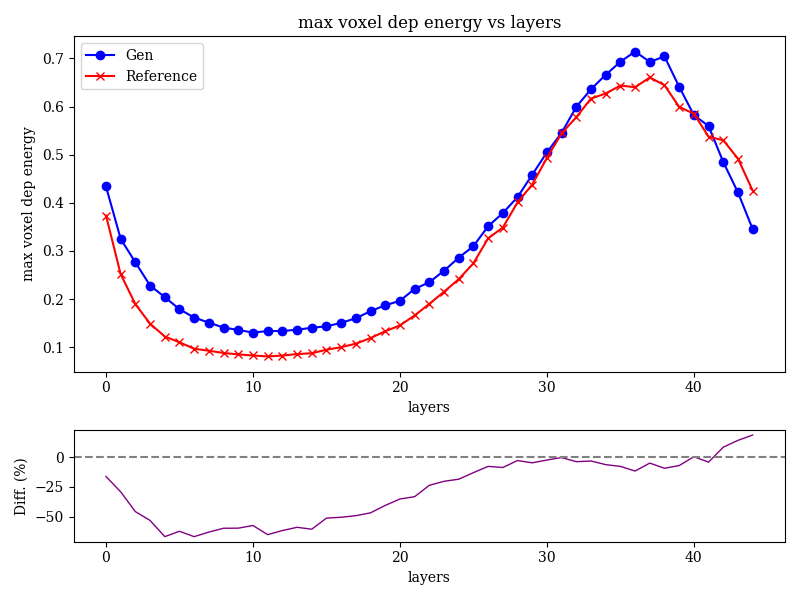
\includegraphics
        [width=\textwidth]{Figures/2_5.png}
        \caption{Max Voxel Deposit vs Layers}
        \label{fig:a2_1}
    \end{subfigure}

    \vspace{0.6cm} % Space between rows

    % Second row: 3 figures
    \begin{subfigure}[b]{0.3\textwidth}  % Adjust width to fit 3 figures
        \centering
        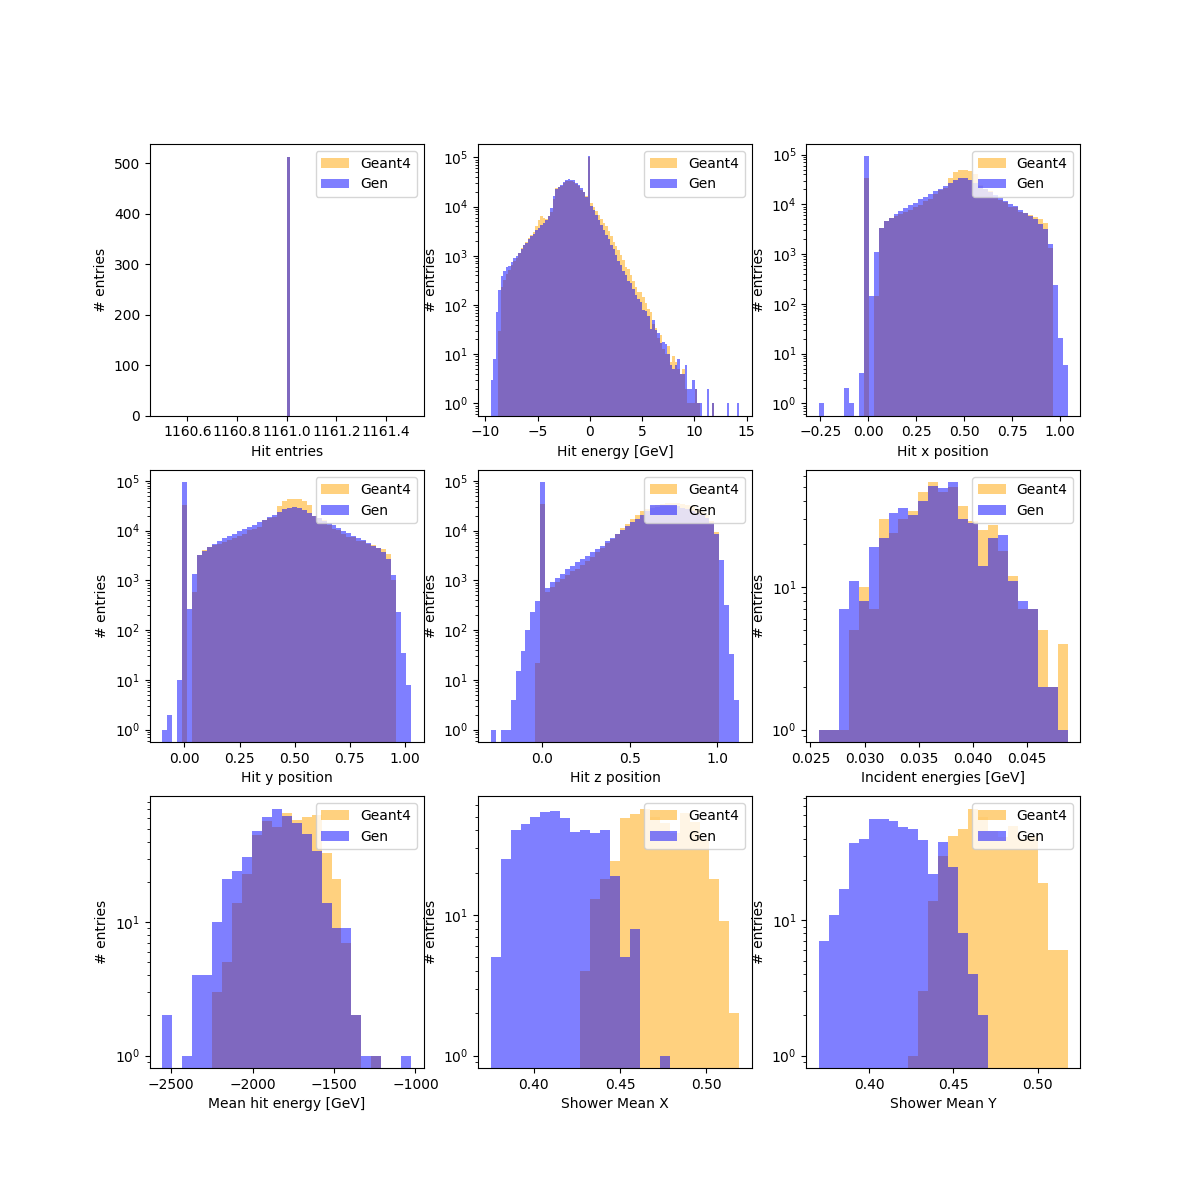
\includegraphics
        [width=\textwidth]{Figures/a2_1.png}
        \caption{1D Histogram}
        \label{fig:a2_5}
    \end{subfigure}
    \hfill
    \begin{subfigure}[b]{0.3\textwidth}
        \centering
        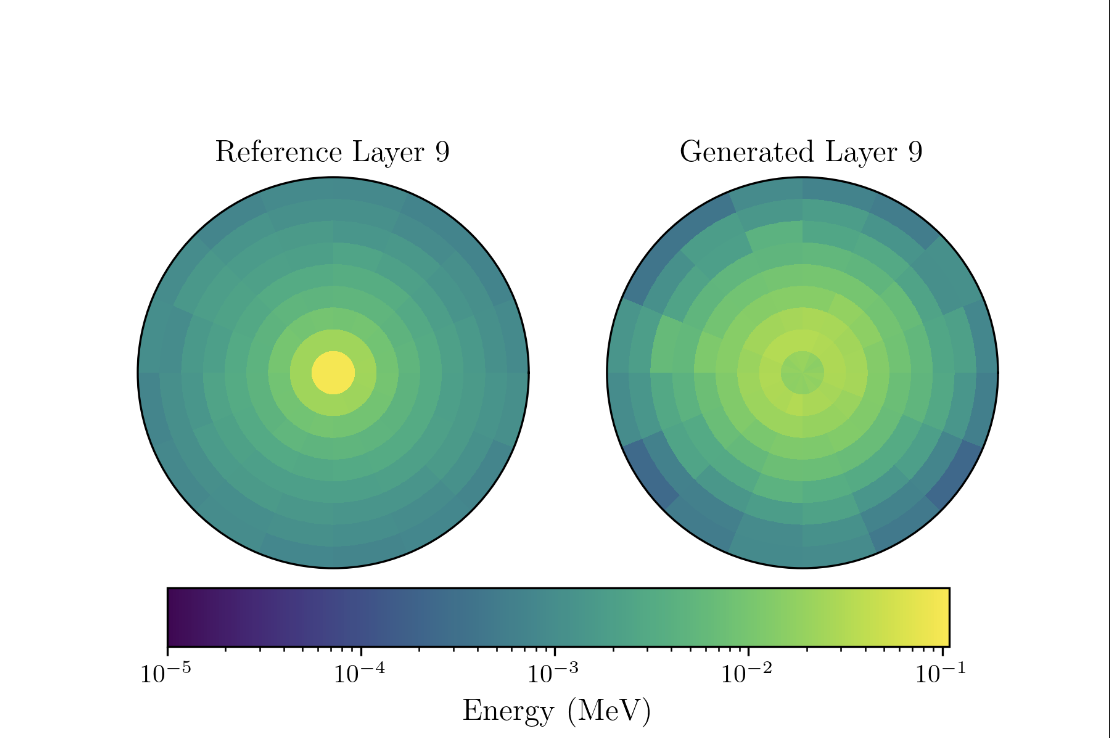
\includegraphics[width=\textwidth]{Figures/a2_5.png}
        \caption{Energy voxel comparison}
        \label{fig:a2_6}
    \end{subfigure}
    \hfill
    \begin{subfigure}[b]{0.3\textwidth}
        \centering
        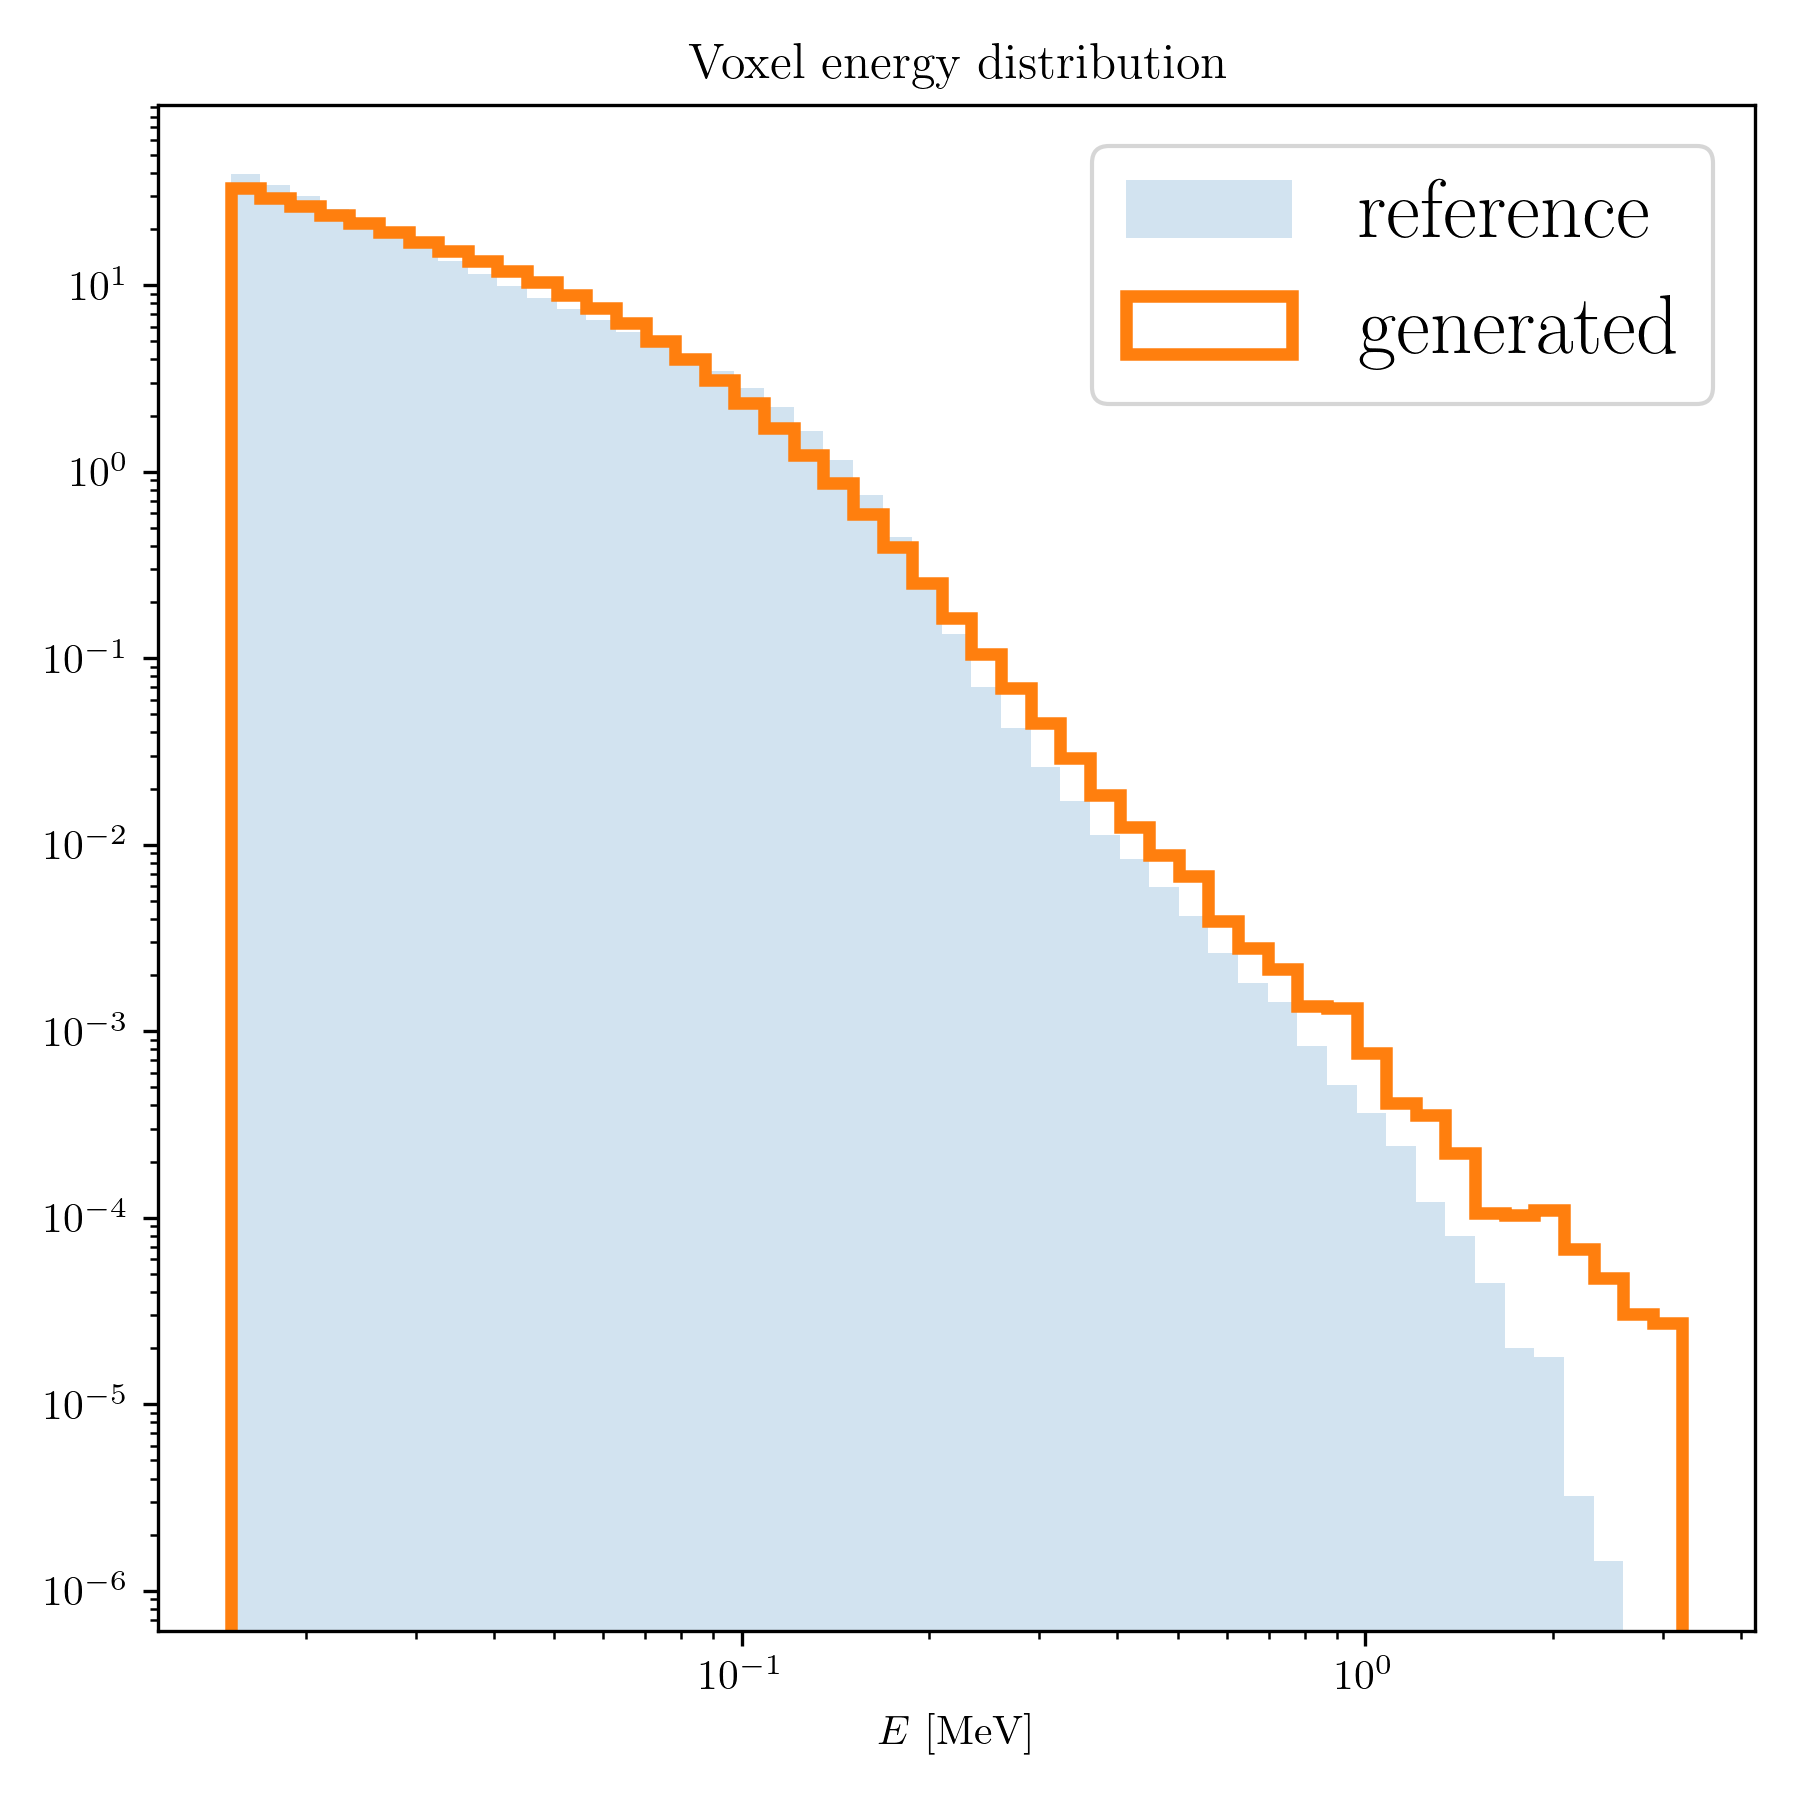
\includegraphics[width=\textwidth]{Figures/a2_6.png}
        \caption{Energy Deposit}
        \label{fig:a2_7}
    \end{subfigure}
\end{figure}
% \section{Result for without using incident energy}
% 7 pictures in total
\newpage
\section{Result for using different Preprocessor}


\begin{figure}[htbp]
    \centering
    % First row: 4 figures
    \begin{subfigure}[b]{0.3\textwidth}
        \centering
        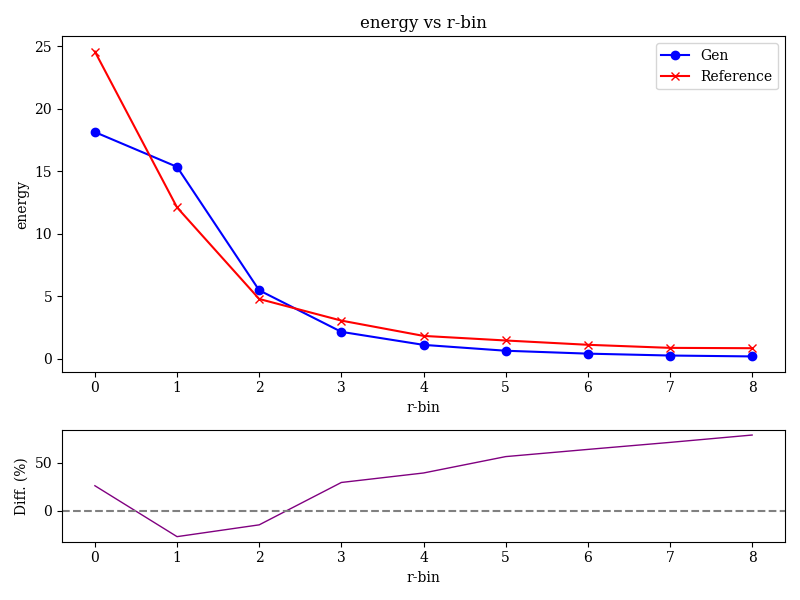
\includegraphics[width=\textwidth]{Figures/robust2.png}
        \caption{Energy vs Radius}
        \label{fig:robust2}
    \end{subfigure}
    \hfill
    \begin{subfigure}[b]{0.3\textwidth}
        \centering
        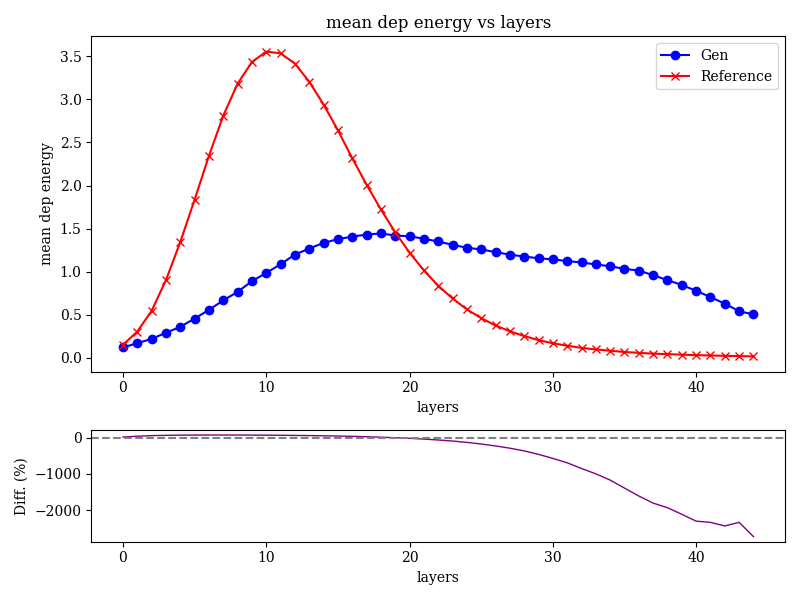
\includegraphics[width=\textwidth]{Figures/robust3.png}
        \caption{Energy vs Z}
        \label{fig:robust3}
    \end{subfigure}
    \hfill
    \begin{subfigure}[b]{0.3\textwidth}
        \centering
        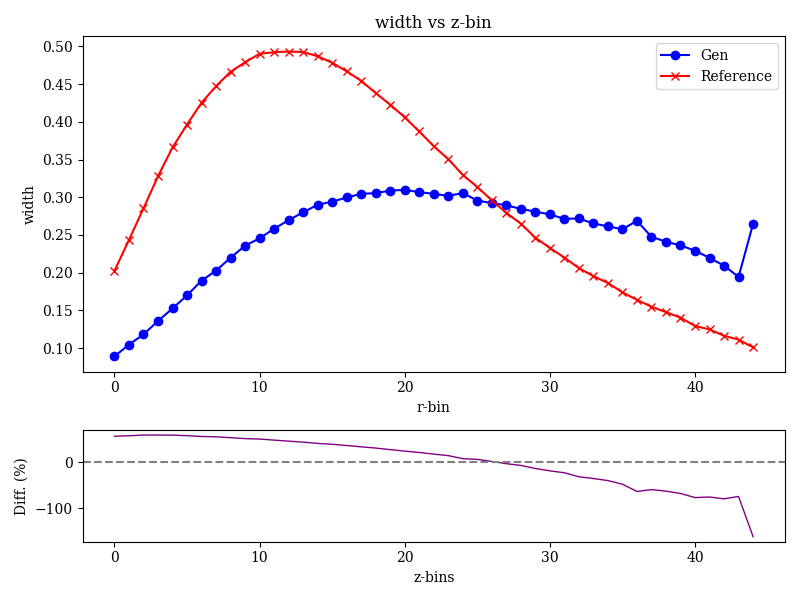
\includegraphics[width=\textwidth]{Figures/robust4.png}
        \caption{R-width vs layers}
        \label{fig:robust4}
    \end{subfigure}
    

    \vspace{0.35cm} % Space between rows

    % Second row: 3 figures
    
    \begin{subfigure}[b]{0.3\textwidth}  % Adjust width to fit 4 figures
        \centering
        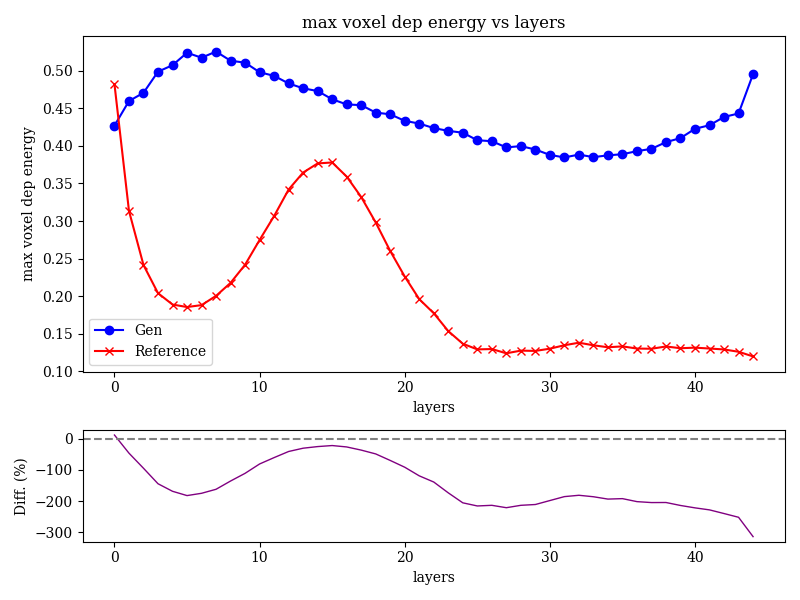
\includegraphics
        [width=\textwidth]{Figures/robust5.png}
        \caption{Max Voxel Deposit vs Layers}
        \label{fig:robust5}
    \end{subfigure}
    \hfill
    \begin{subfigure}[b]{0.3\textwidth}  % Adjust width to fit 3 figures
        \centering
        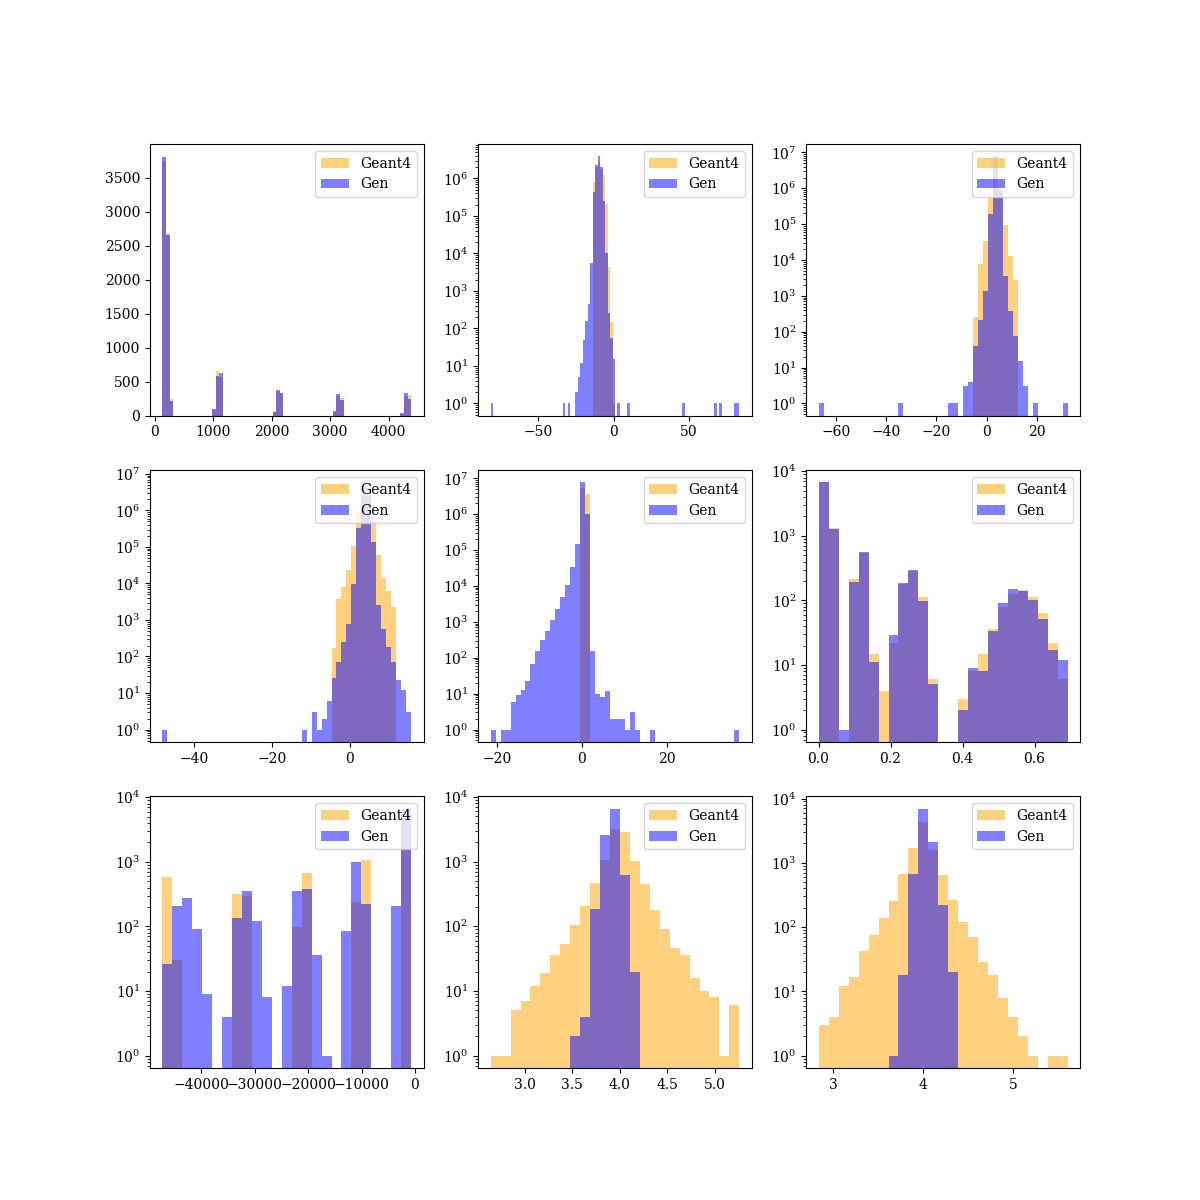
\includegraphics
        [width=\textwidth]{Figures/robust1.png}
        \caption{1D Histogram}
        \label{fig:robust1}
    \end{subfigure}
    \hfill
    \begin{subfigure}[b]{0.3\textwidth}
        \centering
        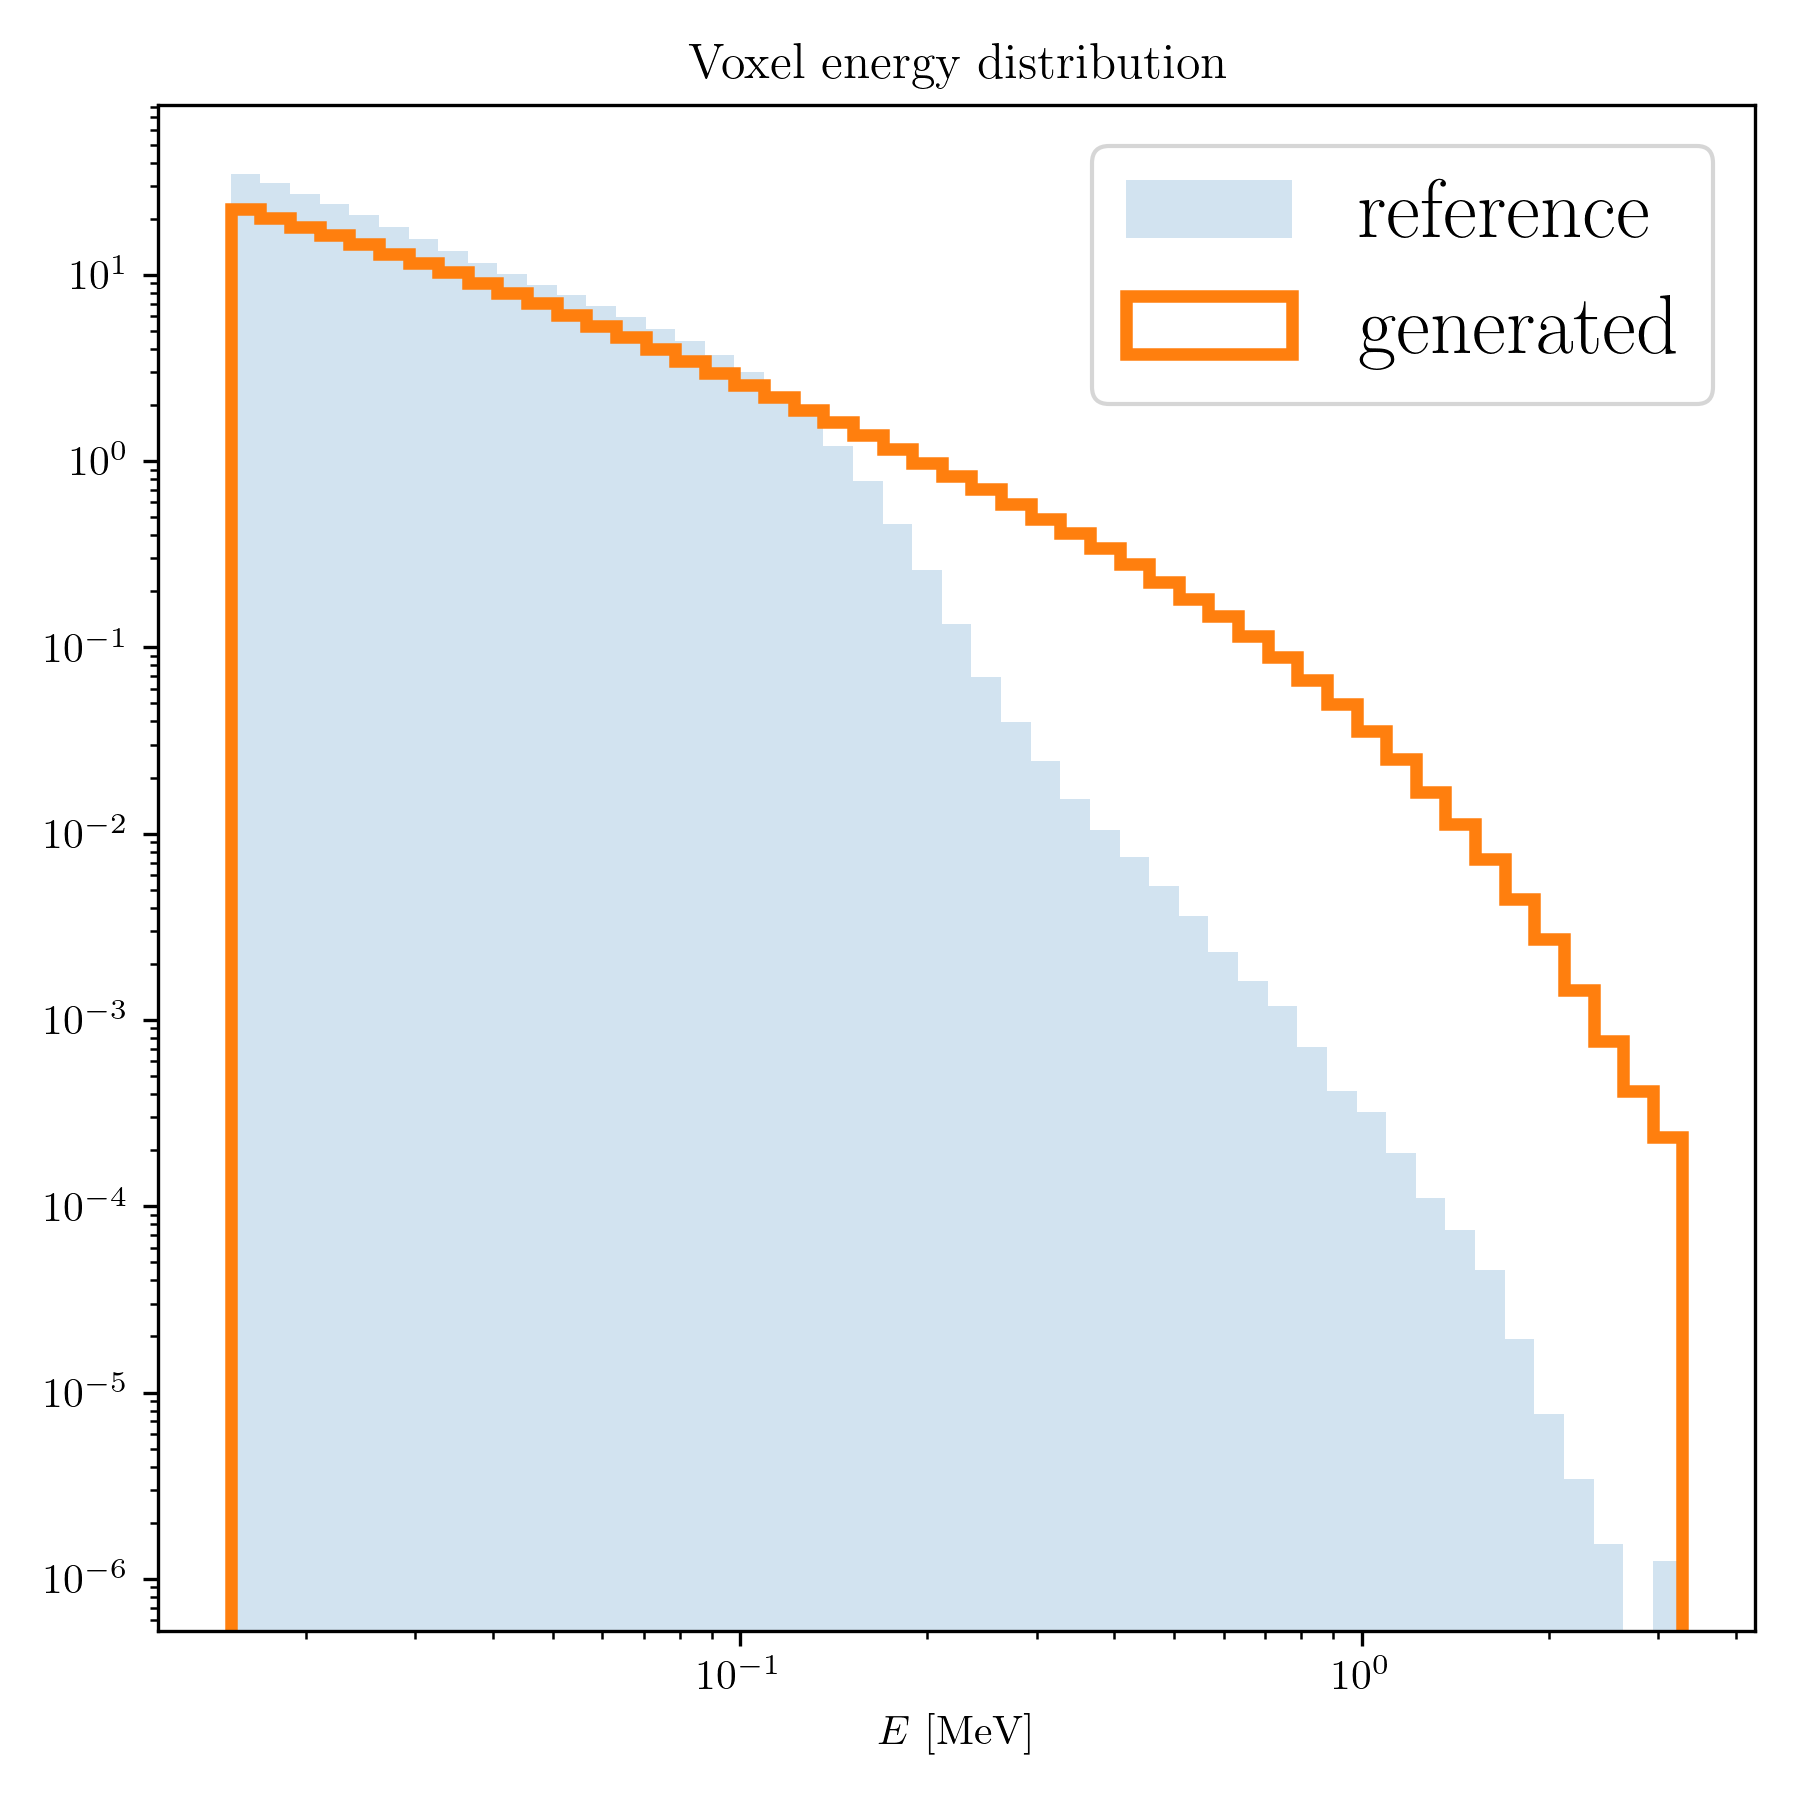
\includegraphics[width=\textwidth]{Figures/robust6.png}
        \caption{Energy Deposit}
        \label{fig:robust6}
    \end{subfigure}
    \caption{Result for using robust preprocessor}
\end{figure}

\begin{figure}
    \centering
    % First row: 4 figures
    \begin{subfigure}[b]{0.3\textwidth}
        \centering
        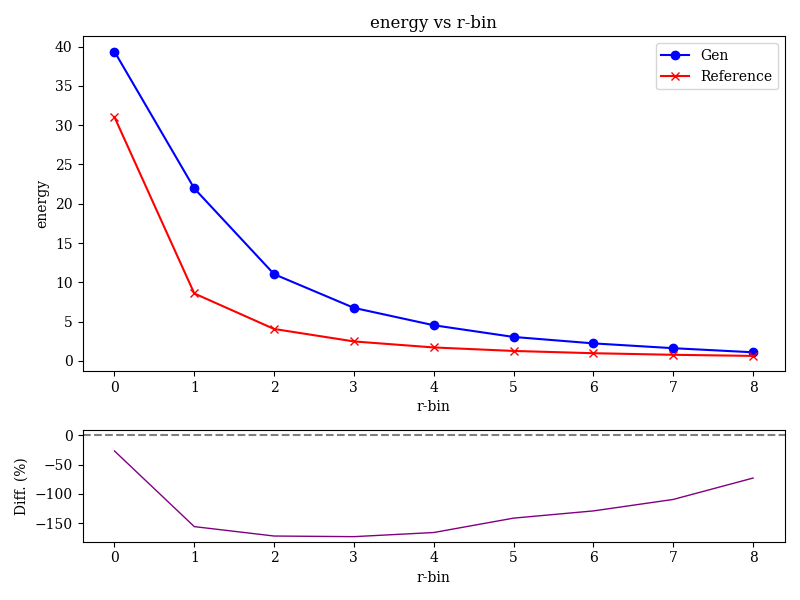
\includegraphics[width=\textwidth]{Figures/quantile2.png}
        \caption{Energy vs Radius}
        \label{fig:quantile2}
    \end{subfigure}
    \hfill
    \begin{subfigure}[b]{0.3\textwidth}
        \centering
        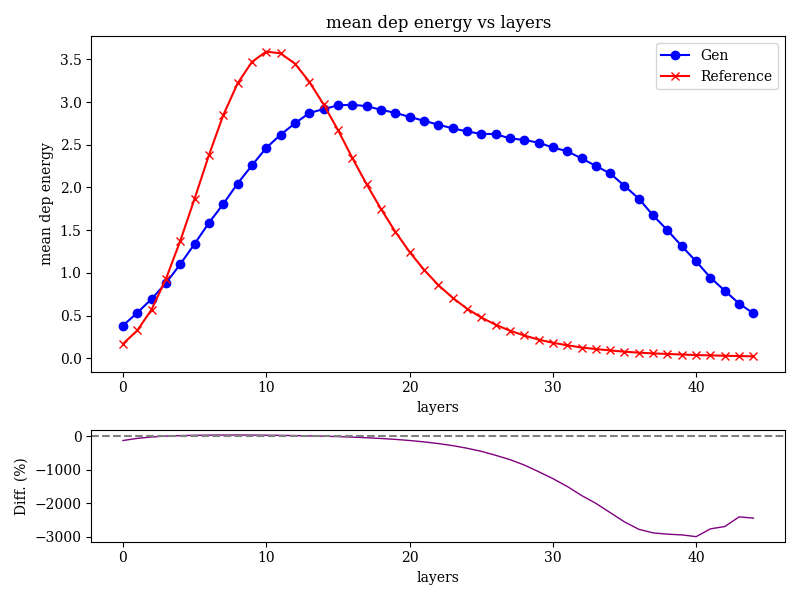
\includegraphics[width=\textwidth]{Figures/quantile3.png}
        \caption{Energy vs Z}
        \label{fig:quantile3}
    \end{subfigure}
    \hfill
    \begin{subfigure}[b]{0.3\textwidth}
        \centering
        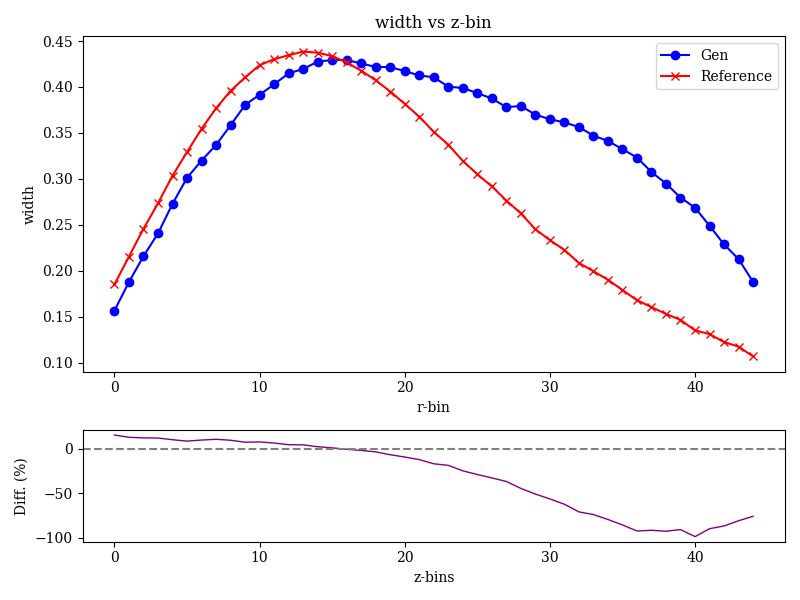
\includegraphics[width=\textwidth]{Figures/quantile4.png}
        \caption{R-width vs layers}
        \label{fig:quantile4}
    \end{subfigure}
    

    \vspace{0.35cm} % Space between rows

    % Second row: 3 figures
    
    \begin{subfigure}[b]{0.3\textwidth}  % Adjust width to fit 4 figures
        \centering
        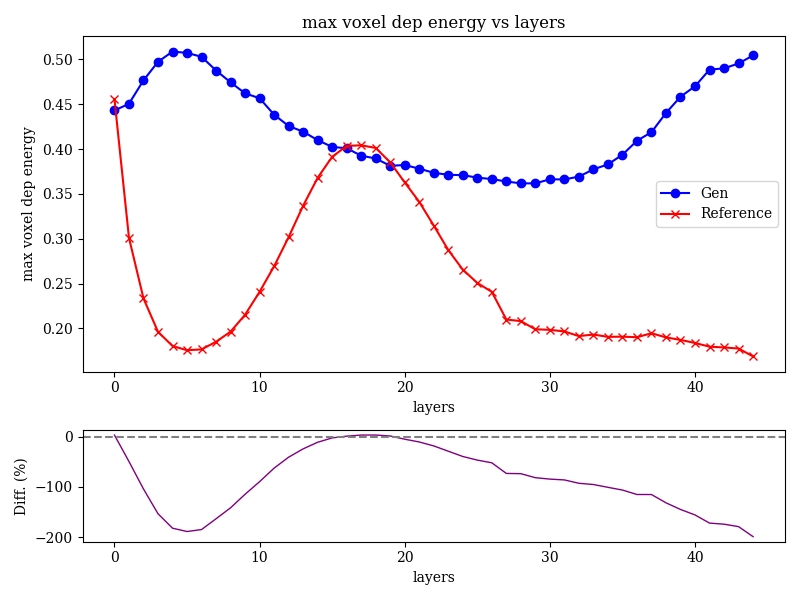
\includegraphics
        [width=\textwidth]{Figures/quantile5.png}
        \caption{Max Voxel Deposit vs Layers}
        \label{fig:quantile5}
    \end{subfigure}
    \hfill
    \begin{subfigure}[b]{0.3\textwidth}  % Adjust width to fit 3 figures
        \centering
        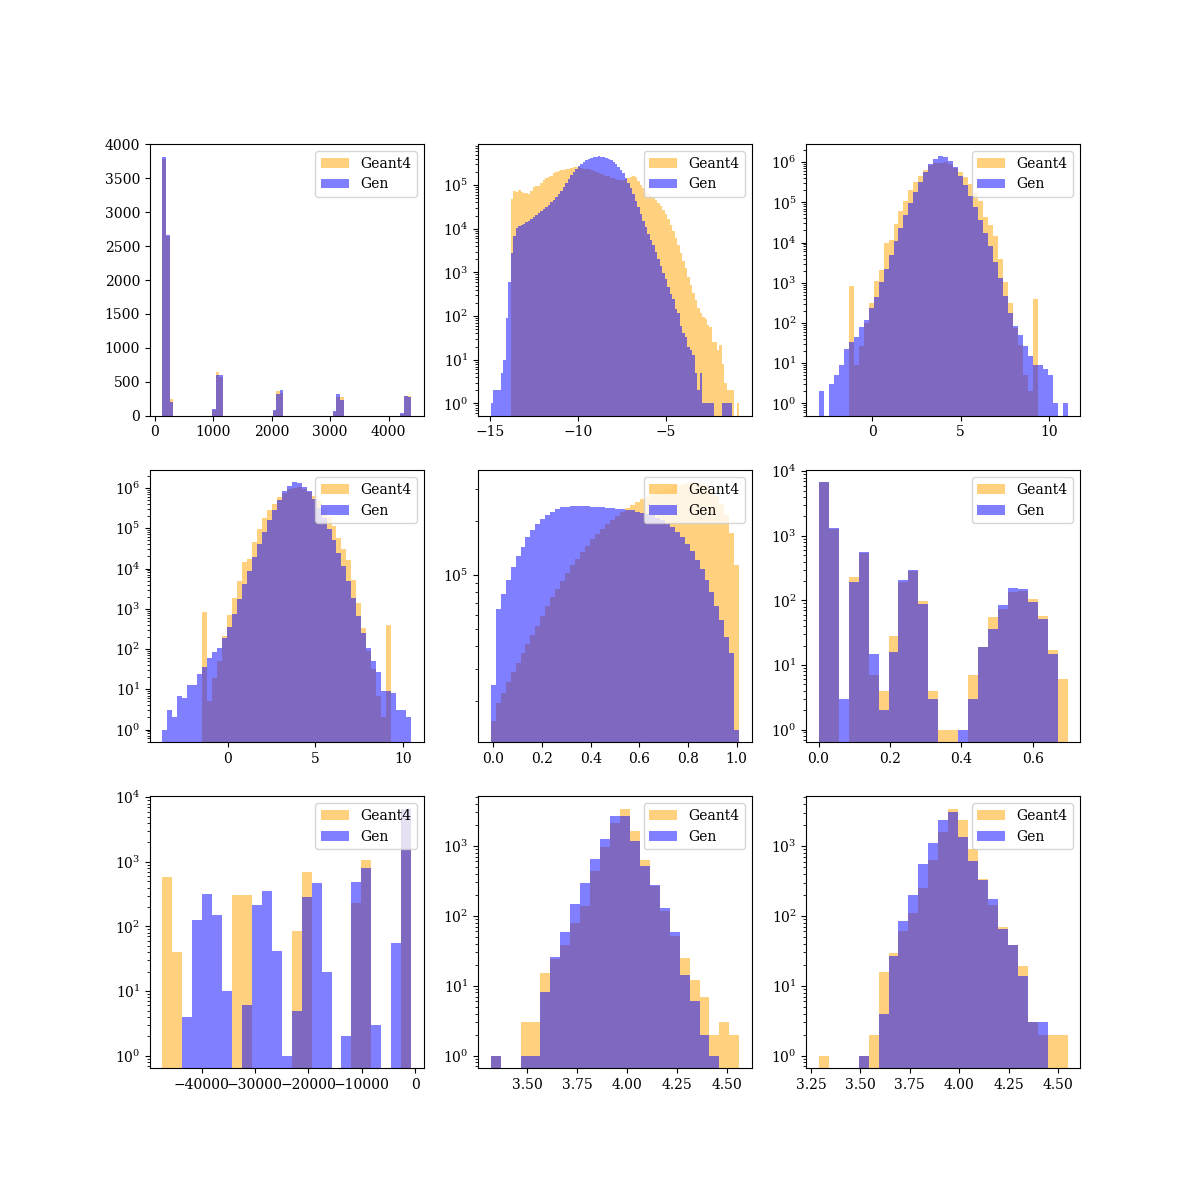
\includegraphics
        [width=\textwidth]{Figures/quantile1.png}
        \caption{1D Histogram}
        \label{fig:quantile1}
    \end{subfigure}
    \hfill
    \begin{subfigure}[b]{0.3\textwidth}
        \centering
        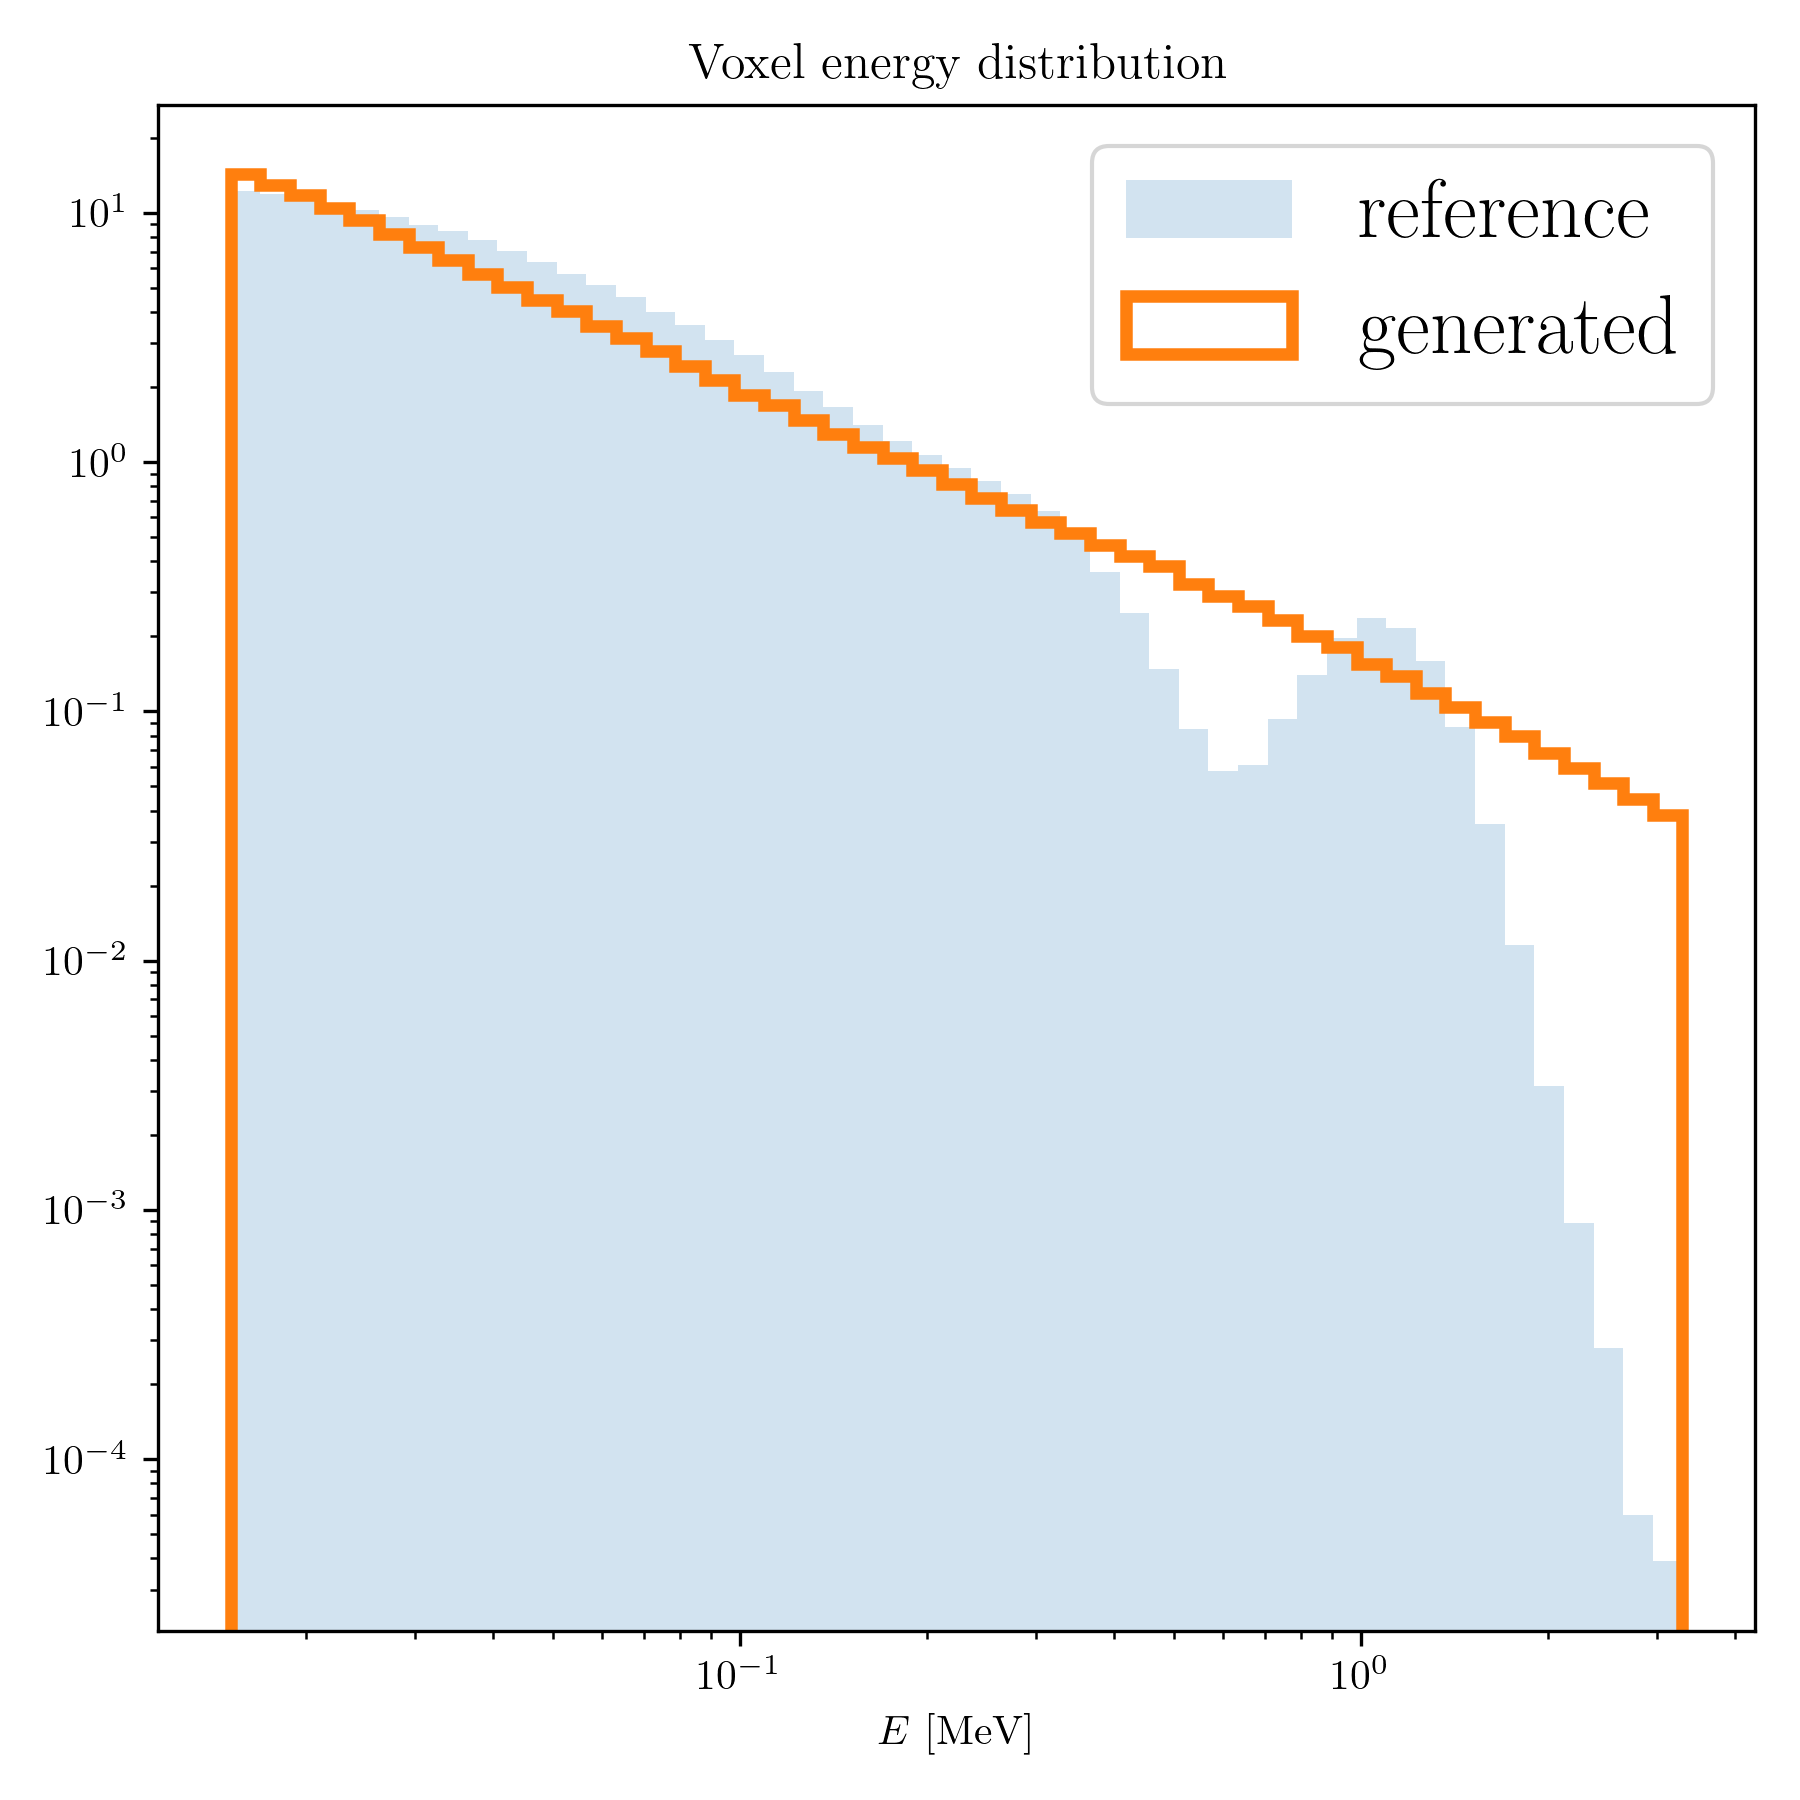
\includegraphics[width=\textwidth]{Figures/quantile6.png}
        \caption{Energy Deposit}
        \label{fig:quantile6}
    \end{subfigure}
    \caption{Result for using quantile preprocessor}
\end{figure}

\begin{figure}
    \centering
    % First row: 4 figures
    \begin{subfigure}[b]{0.3\textwidth}
        \centering
        \includegraphics[width=\textwidth]{Figures/exponential2.png}
        \caption{Energy vs Radius}
        \label{fig:exp2}
    \end{subfigure}
    \hfill
    \begin{subfigure}[b]{0.3\textwidth}
        \centering
        \includegraphics[width=\textwidth]{Figures/exponential3.png}
        \caption{Energy vs Z}
        \label{fig:exp3}
    \end{subfigure}
    \hfill
    \begin{subfigure}[b]{0.3\textwidth}
        \centering
        \includegraphics[width=\textwidth]{Figures/exponential4.png}
        \caption{R-width vs layers}
        \label{fig:exp4}
    \end{subfigure}
    

    \vspace{0.35cm} % Space between rows

    % Second row: 3 figures
    
    \begin{subfigure}[b]{0.3\textwidth}  % Adjust width to fit 4 figures
        \centering
        \includegraphics
        [width=\textwidth]{Figures/a1_5.png}
        \caption{Max Voxel Deposit vs Layers}
        \label{fig:exp5}
    \end{subfigure}
    \hfill
    \begin{subfigure}[b]{0.3\textwidth}  % Adjust width to fit 3 figures
        \centering
        \includegraphics
        [width=\textwidth]{Figures/exponential1.png}
        \caption{1D Histogram}
        \label{fig:exp1}
    \end{subfigure}
    \hfill
    \begin{subfigure}[b]{0.3\textwidth}
        \centering
        \includegraphics[width=\textwidth]{Figures/exponential6.png}
        \caption{Energy Deposit}
        \label{fig:exp6}
    \end{subfigure}
    \caption{Result for using exponential preprocessor}
\end{figure}

\newpage
\section{Result for using different SDE settings}
every 7 pictures for VE,VP for sde =1,5,10,20. Total 7*2*4=56 pictures

\begin{figure}[bthp]
    \centering
    % First row: 4 figures
    \begin{subfigure}[b]{0.23\textwidth}
        \centering
        \includegraphics[width=\textwidth]{Figures/ve20_2.png}
        \caption{$\sigma_{max}=20$}
        \label{fig:ve20_2}
    \end{subfigure}
    \hfill
    \begin{subfigure}[b]{0.23\textwidth}
        \centering
        \includegraphics[width=\textwidth]{Figures/ve10_2.png}
        \caption{$\sigma_{max}=10$}
        \label{fig:ve10_2}
    \end{subfigure}
    \hfill
    \begin{subfigure}[b]{0.23\textwidth}
        \centering
        \includegraphics[width=\textwidth]{Figures/ve5_2.png}
        \caption{$\sigma_{max}=5$}
        \label{fig:ve5_2}
    \end{subfigure}
    \hfill
    \begin{subfigure}[b]{0.23\textwidth}  % Adjust width to fit 4 figures
        \centering
        \includegraphics[width=\textwidth]{Figures/ve1_2.png}
        \caption{$\sigma_{max}=1$}
        \label{fig:ve1_2}
    \end{subfigure}
    \caption{Result for Energy vs Radius for VE}
\end{figure}

\begin{figure}[bthp]
    \centering
    % First row: 4 figures
    \begin{subfigure}[b]{0.23\textwidth}
        \centering
        \includegraphics[width=\textwidth]{Figures/vp20_2.png}
        \caption{$\sigma_{max}=20$}
        \label{fig:vp20_2}
    \end{subfigure}
    \hfill
    \begin{subfigure}[b]{0.23\textwidth}
        \centering
        \includegraphics[width=\textwidth]{Figures/vp10_2.png}
        \caption{$\sigma_{max}=10$}
        \label{fig:vp10_2}
    \end{subfigure}
    \hfill
    \begin{subfigure}[b]{0.23\textwidth}
        \centering
        \includegraphics[width=\textwidth]{Figures/vp5_2.png}
        \caption{$\sigma_{max}=5$}
        \label{fig:vp5_2}
    \end{subfigure}
    \hfill
    \begin{subfigure}[b]{0.23\textwidth}  % Adjust width to fit 4 figures
        \centering
        \includegraphics[width=\textwidth]{Figures/vp1_2.png}
        \caption{$\sigma_{max}=1$}
        \label{fig:vp1_2}
    \end{subfigure}
    \caption{Result for Energy vs Radius for VP}
\end{figure}

\begin{figure}[bthp]
    \centering
    % First row: 4 figures
    \begin{subfigure}[b]{0.23\textwidth}
        \centering
        \includegraphics[width=\textwidth]{Figures/ve20_3.png}
        \caption{$\sigma_{max}=20$}
        \label{fig:ve20_3}
    \end{subfigure}
    \hfill
    \begin{subfigure}[b]{0.23\textwidth}
        \centering
        \includegraphics[width=\textwidth]{Figures/ve10_3.png}
        \caption{$\sigma_{max}=10$}
        \label{fig:ve10_3}
    \end{subfigure}
    \hfill
    \begin{subfigure}[b]{0.23\textwidth}
        \centering
        \includegraphics[width=\textwidth]{Figures/ve5_3.png}
        \caption{$\sigma_{max}=5$}
        \label{fig:ve5_3}
    \end{subfigure}
    \hfill
    \begin{subfigure}[b]{0.23\textwidth}  % Adjust width to fit 4 figures
        \centering
        \includegraphics[width=\textwidth]{Figures/ve1_3.png}
        \caption{$\sigma_{max}=1$}
        \label{fig:ve1_3}
    \end{subfigure}
    \caption{Result for Energy vs Layers for VE}
\end{figure}

\begin{figure}[bthp]
    \centering
    % First row: 4 figures
    \begin{subfigure}[b]{0.23\textwidth}
        \centering
        \includegraphics[width=\textwidth]{Figures/vp20_3.png}
        \caption{$\sigma_{max}=20$}
        \label{fig:vp20_3}
    \end{subfigure}
    \hfill
    \begin{subfigure}[b]{0.23\textwidth}
        \centering
        \includegraphics[width=\textwidth]{Figures/vp10_3.png}
        \caption{$\sigma_{max}=10$}
        \label{fig:vp10_3}
    \end{subfigure}
    \hfill
    \begin{subfigure}[b]{0.23\textwidth}
        \centering
        \includegraphics[width=\textwidth]{Figures/vp5_3.png}
        \caption{$\sigma_{max}=5$}
        \label{fig:vp5_3}
    \end{subfigure}
    \hfill
    \begin{subfigure}[b]{0.23\textwidth}  % Adjust width to fit 4 figures
        \centering
        \includegraphics[width=\textwidth]{Figures/vp1_3.png}
        \caption{$\sigma_{max}=1$}
        \label{fig:vp1_3}
    \end{subfigure}
    \caption{Result for Energy vs Layers for VP}
\end{figure}

\begin{figure}[bthp]
    \centering
    % First row: 4 figures
    \begin{subfigure}[b]{0.23\textwidth}
        \centering
        \includegraphics[width=\textwidth]{Figures/ve20_4.png}
        \caption{$\sigma_{max}=20$}
        \label{fig:ve20_4}
    \end{subfigure}
    \hfill
    \begin{subfigure}[b]{0.23\textwidth}
        \centering
        \includegraphics[width=\textwidth]{Figures/ve10_4.png}
        \caption{$\sigma_{max}=10$}
        \label{fig:ve10_4}
    \end{subfigure}
    \hfill
    \begin{subfigure}[b]{0.23\textwidth}
        \centering
        \includegraphics[width=\textwidth]{Figures/ve5_4.png}
        \caption{$\sigma_{max}=5$}
        \label{fig:ve5_4}
    \end{subfigure}
    \hfill
    \begin{subfigure}[b]{0.23\textwidth}  % Adjust width to fit 4 figures
        \centering
        \includegraphics[width=\textwidth]{Figures/ve1_4.png}
        \caption{$\sigma_{max}=1$}
        \label{fig:ve1_4}
    \end{subfigure}
    \caption{Result for R-width vs Layers for VE}
\end{figure}

\begin{figure}[bthp]
    \centering
    % First row: 4 figures
    \begin{subfigure}[b]{0.23\textwidth}
        \centering
        \includegraphics[width=\textwidth]{Figures/vp20_4.png}
        \caption{$\sigma_{max}=20$}
        \label{fig:vp20_4}
    \end{subfigure}
    \hfill
    \begin{subfigure}[b]{0.23\textwidth}
        \centering
        \includegraphics[width=\textwidth]{Figures/vp10_4.png}
        \caption{$\sigma_{max}=10$}
        \label{fig:vp10_4}
    \end{subfigure}
    \hfill
    \begin{subfigure}[b]{0.23\textwidth}
        \centering
        \includegraphics[width=\textwidth]{Figures/vp5_4.png}
        \caption{$\sigma_{max}=5$}
        \label{fig:vp5_4}
    \end{subfigure}
    \hfill
    \begin{subfigure}[b]{0.23\textwidth}  % Adjust width to fit 4 figures
        \centering
        \includegraphics[width=\textwidth]{Figures/vp1_4.png}
        \caption{$\sigma_{max}=1$}
        \label{fig:vp1_4}
    \end{subfigure}
    \caption{Result for R-width vs Layers for VP}
\end{figure}

\begin{figure}[bthp]
    \centering
    % First row: 4 figures
    \begin{subfigure}[b]{0.23\textwidth}
        \centering
        \includegraphics[width=\textwidth]{Figures/ve20_5.png}
        \caption{$\sigma_{max}=20$}
        \label{fig:ve20_5}
    \end{subfigure}
    \hfill
    \begin{subfigure}[b]{0.23\textwidth}
        \centering
        \includegraphics[width=\textwidth]{Figures/ve10_5.png}
        \caption{$\sigma_{max}=10$}
        \label{fig:ve10_5}
    \end{subfigure}
    \hfill
    \begin{subfigure}[b]{0.23\textwidth}
        \centering
        \includegraphics[width=\textwidth]{Figures/ve5_5.png}
        \caption{$\sigma_{max}=5$}
        \label{fig:ve5_5}
    \end{subfigure}
    \hfill
    \begin{subfigure}[b]{0.23\textwidth}  % Adjust width to fit 4 figures
        \centering
        \includegraphics[width=\textwidth]{Figures/ve1_5.png}
        \caption{$\sigma_{max}=1$}
        \label{fig:ve1_5}
    \end{subfigure}
    \caption{Result for Max Voxel Deposit vs Layer for VE}
\end{figure}

\begin{figure}
    \centering
    % First row: 4 figures
    \begin{subfigure}[b]{0.23\textwidth}
        \centering
        \includegraphics[width=\textwidth]{Figures/vp20_5.png}
        \caption{$\sigma_{max}=20$}
        \label{fig:vp20_5}
    \end{subfigure}
    \hfill
    \begin{subfigure}[b]{0.23\textwidth}
        \centering
        \includegraphics[width=\textwidth]{Figures/vp10_5.png}
        \caption{$\sigma_{max}=10$}
        \label{fig:vp10_5}
    \end{subfigure}
    \hfill
    \begin{subfigure}[b]{0.23\textwidth}
        \centering
        \includegraphics[width=\textwidth]{Figures/vp5_5.png}
        \caption{$\sigma_{max}=5$}
        \label{fig:vp5_5}
    \end{subfigure}
    \hfill
    \begin{subfigure}[b]{0.23\textwidth}  % Adjust width to fit 4 figures
        \centering
        \includegraphics[width=\textwidth]{Figures/vp1_5.png}
        \caption{$\sigma_{max}=1$}
        \label{fig:vp1_5}
    \end{subfigure}
    \caption{Result for Max Voxel Deposit vs Layer for VP}
\end{figure}

\begin{figure}
    \centering
    % First row: 4 figures
    \begin{subfigure}[b]{0.23\textwidth}
        \centering
        \includegraphics[width=\textwidth]{Figures/ve20_1dpng.png}
        \caption{$\sigma_{max}=20$}
        \label{fig:ve20_1}
    \end{subfigure}
    \hfill
    \begin{subfigure}[b]{0.23\textwidth}
        \centering
        \includegraphics[width=\textwidth]{Figures/ve10_1.png}
        \caption{$\sigma_{max}=10$}
        \label{fig:ve10_1}
    \end{subfigure}
    \hfill
    \begin{subfigure}[b]{0.23\textwidth}
        \centering
        \includegraphics[width=\textwidth]{Figures/ve5_1.png}
        \caption{$\sigma_{max}=5$}
        \label{fig:ve5_1}
    \end{subfigure}
    \hfill
    \begin{subfigure}[b]{0.23\textwidth}  % Adjust width to fit 4 figures
        \centering
        \includegraphics[width=\textwidth]{Figures/ve1_1.png}
        \caption{$\sigma_{max}=1$}
        \label{fig:ve1_1}
    \end{subfigure}
    \caption{Result for Each Dimension VE}
\end{figure}

\begin{figure}
    \centering
    % First row: 4 figures
    \begin{subfigure}[b]{0.23\textwidth}
        \centering
        \includegraphics[width=\textwidth]{Figures/vp20_1.png}
        \caption{$\sigma_{max}=20$}
        \label{fig:vp20_1}
    \end{subfigure}
    \hfill
    \begin{subfigure}[b]{0.23\textwidth}
        \centering
        \includegraphics[width=\textwidth]{Figures/vp10_1.png}
        \caption{$\sigma_{max}=10$}
        \label{fig:vp10_1}
    \end{subfigure}
    \hfill
    \begin{subfigure}[b]{0.23\textwidth}
        \centering
        \includegraphics[width=\textwidth]{Figures/vp5_1.png}
        \caption{$\sigma_{max}=5$}
        \label{fig:vp5_1}
    \end{subfigure}
    \hfill
    \begin{subfigure}[b]{0.23\textwidth}  % Adjust width to fit 4 figures
        \centering
        \includegraphics[width=\textwidth]{Figures/vp1_1.png}
        \caption{$\sigma_{max}=1$}
        \label{fig:vp1_1}
    \end{subfigure}
    \caption{Result for Each Dimension VP}
\end{figure}

\begin{figure}
    \centering
    % First row: 4 figures
    \begin{subfigure}[b]{0.23\textwidth}
        \centering
        \includegraphics[width=\textwidth]{Figures/ve20_6.png}
        \caption{$\sigma_{max}=20$}
        \label{fig:ve20_6}
    \end{subfigure}
    \hfill
    \begin{subfigure}[b]{0.23\textwidth}
        \centering
        \includegraphics[width=\textwidth]{Figures/ve10_6.png}
        \caption{$\sigma_{max}=10$}
        \label{fig:ve10_6}
    \end{subfigure}
    \hfill
    \begin{subfigure}[b]{0.23\textwidth}
        \centering
        \includegraphics[width=\textwidth]{Figures/ve5_6.png}
        \caption{$\sigma_{max}=5$}
        \label{fig:ve5_6}
    \end{subfigure}
    \hfill
    \begin{subfigure}[b]{0.23\textwidth}  % Adjust width to fit 4 figures
        \centering
        \includegraphics[width=\textwidth]{Figures/ve1_6.png}
        \caption{$\sigma_{max}=1$}
        \label{fig:ve1_6}
    \end{subfigure}
    \caption{Result for Energy Voxel Comparison for VE}
\end{figure}

\begin{figure}
    \centering
    % First row: 4 figures
    \begin{subfigure}[b]{0.23\textwidth}
        \centering
        \includegraphics[width=\textwidth]{Figures/vp20_6.png}
        \caption{$\sigma_{max}=20$}
        \label{fig:vp20_6}
    \end{subfigure}
    \hfill
    \begin{subfigure}[b]{0.23\textwidth}
        \centering
        \includegraphics[width=\textwidth]{Figures/vp10_6.png}
        \caption{$\sigma_{max}=10$}
        \label{fig:vp10_6}
    \end{subfigure}
    \hfill
    \begin{subfigure}[b]{0.23\textwidth}
        \centering
        \includegraphics[width=\textwidth]{Figures/vp5_6.png}
        \caption{$\sigma_{max}=5$}
        \label{fig:vp5_6}
    \end{subfigure}
    \hfill
    \begin{subfigure}[b]{0.23\textwidth}  % Adjust width to fit 4 figures
        \centering
        \includegraphics[width=\textwidth]{Figures/vp1_6.png}
        \caption{$\sigma_{max}=1$}
        \label{fig:vp1_6}
    \end{subfigure}
    \caption{Result for Energy Voxel Comparison for VP}
\end{figure}

\begin{figure}
    \centering
    % First row: 4 figures
    \begin{subfigure}[b]{0.23\textwidth}
        \centering
        \includegraphics[width=\textwidth]{Figures/ve20_7.png}
        \caption{$\sigma_{max}=20$}
        \label{fig:ve20_7}
    \end{subfigure}
    \hfill
    \begin{subfigure}[b]{0.23\textwidth}
        \centering
        \includegraphics[width=\textwidth]{Figures/ve10_7.png}
        \caption{$\sigma_{max}=10$}
        \label{fig:ve10_7}
    \end{subfigure}
    \hfill
    \begin{subfigure}[b]{0.23\textwidth}
        \centering
        \includegraphics[width=\textwidth]{Figures/ve5_7.png}
        \caption{$\sigma_{max}=5$}
        \label{fig:ve5_7}
    \end{subfigure}
    \hfill
    \begin{subfigure}[b]{0.23\textwidth}  % Adjust width to fit 4 figures
        \centering
        \includegraphics[width=\textwidth]{Figures/ve1_7.png}
        \caption{$\sigma_{max}=1$}
        \label{fig:ve1_7}
    \end{subfigure}
    \caption{Result for Energy Deposit for VE}
\end{figure}

\begin{figure}
    \centering
    % First row: 4 figures
    \begin{subfigure}[b]{0.23\textwidth}
        \centering
        \includegraphics[width=\textwidth]{Figures/vp20_7.png}
        \caption{$\sigma_{max}=20$}
        \label{fig:vp20_7}
    \end{subfigure}
    \hfill
    \begin{subfigure}[b]{0.23\textwidth}
        \centering
        \includegraphics[width=\textwidth]{Figures/vp10_7.png}
        \caption{$\sigma_{max}=10$}
        \label{fig:vp10_7}
    \end{subfigure}
    \hfill
    \begin{subfigure}[b]{0.23\textwidth}
        \centering
        \includegraphics[width=\textwidth]{Figures/vp5_7.png}
        \caption{$\sigma_{max}=5$}
        \label{fig:vp5_7}
    \end{subfigure}
    \hfill
    \begin{subfigure}[b]{0.23\textwidth}  % Adjust width to fit 4 figures
        \centering
        \includegraphics[width=\textwidth]{Figures/vp1_7.png}
        \caption{$\sigma_{max}=1$}
        \label{fig:vp1_7}
    \end{subfigure}
    \caption{Result for Energy Deposit for VP}
\end{figure}

% B. Timing resolution
% % Appendix A

\chapter{TopFCNH} % Main appendix title

\label{AppendixB} % For referencing this appendix elsewhere, use \ref{AppendixA}

% outline
%----------------------------------------------------------------------------
% 
%
\section{Introduction}

Besides my work on the Fast Calorimeter Simulation Challenge, I have also been involved in the TopFCNH project. For the sake of better understanding the concept and workflow of an analysis. This project aims to study the the interaction between top quark, higgs boson, and a light quark (u or c) in the context of the Standard Model Effective Field Theory (SMEFT) and search for new physics phenomena. It's just at the beginning stage, so what I have done includes roundtable presentation, gridpack preparation, monte carlo and data comparison. In this appendix, I will provide an overview of the TopFCNC project, the analysis workflow, gridpack generation, and the current status of the project.

\section{Background}

While higgs boson has been discovered in 2012, which is the newest particle, and the LHC is mainly designed for observing it, the top quark is the heaviest known elementary particle in the Standard Model (SM). The interaction between top quark and higgs boson is of great interest, as it can provide many insights into many unknown field.

The top-quark flavor-changing neutral current (TopFCNC) decay $t \to Hq$ (where $q = u, c$) is highly suppressed in the Standard Model (SM) due to the Glashow-Iliopoulos-Maiani (GIM) mechanism. \cite{maiani_gim_2013} The predicted SM branching ratio for this process is $BR(t \to Hq) \sim 10^{-15} - 10^{-13}$, making it practically unobservable at the LHC. However, many beyond-the-SM (BSM) theories predict significantly enhanced branching ratios, making it a promising channel for new physics searches. As you can see the figure \ref{fig:TopFCNC}

\begin{figure}[htbp]
    \centering
    \includegraphics[width=0.8\textwidth]{Figures/topfcnc.png}
    \caption{The prediction and the result so far}
    \label{fig:TopFCNC}
\end{figure}

Several BSM frameworks predict an increase in the branching ratio. The Two-Higgs Doublet Model (2HDM) suggests that $BR(t \to Hq)$ could reach $10^{-5} - 10^{-3}$.\cite{noauthor_fcnchistory_nodate} Similarly, Supersymmetric Models (SUSY) predict comparable enhancements. Additionally, theories involving a Composite Higgs and Extra Dimensions indicate the possibility of increasing the branching ratio to $10^{-4} - 10^{-3}$. Given these enhancements, detecting $t \to Hq$ at the LHC would be a clear sign of new physics.

Among the Higgs boson decay channels, the $H \to \gamma\gamma$ (diphoton decay) is particularly attractive due to its clean experimental signature in the CMS electromagnetic calorimeter. The branching ratio of $H \to \gamma\gamma$ for a 125 GeV Higgs is approximately $0.2\%$, which is small but provides a well-reconstructed final state. Our research focuses on the process $pp \to t\bar{t}, t \to Hq, H \to \gamma\gamma$, where the diphoton final state can be efficiently detected using high-resolution electromagnetic calorimetry.

Photon triggers in CMS have high efficiency, with single-photon triggers reaching efficiencies above $99\%$ and double-photon triggers capturing over $88\%$ of events. Major backgrounds include prompt diphoton production ($pp \to \gamma\gamma + \text{jets}$) and fake $\gamma + j $, which can be reduced by later analysis methods.

\section{Analysis Workflow}
\section{Gridpack Generation}
\section{Current Status}


%----------------------------------------------------------------------------------------
%	BIBLIOGRAPHY
%----------------------------------------------------------------------------------------

\printbibliography[heading=bibintoc]

%----------------------------------------------------------------------------------------
%	INDEX
%----------------------------------------------------------------------------------------

\printindex

%----------------------------------------------------------------------------------------

\end{document}
